\documentclass[11pt,twoside]{amsbook}
\usepackage[left=4cm,top=3.5cm,bottom=3.5cm,right=3cm]{geometry}
\usepackage[latin1]{inputenc}
%\usepackage{ramo,smcapt1}
%\usepackage[latin1]{inputenc}
%%\usepackage[dvipdfm]{hyperref}
\usepackage{array}
\usepackage{amsmath,arydshln}
\usepackage{MnSymbol}%
\usepackage{wasysym}%
\usepackage{enumerate}
\usepackage{cancel} 
%\usepackage{amsfonts}
%\usepackage{multirow} 
\usepackage{tikz}
\usetikzlibrary{shapes,arrows}
\usepackage{multirow}
\usepackage{lscape}
\usepackage{epstopdf}
\usepackage{booktabs}
\usepackage{hhline}
%\usepackage{pgfplots}
%\usepackage{etex}
%\usepackage{comment}
%\usepackage{rotating}
%\usepackage{morefloats}
%\setlength{\rotFPtop}{0pt plus 1fil}
%\reserveinserts{18}
%\usepackage{morefloats}
%\usetikzlibrary{backgrounds,decorations.pathmorphing}
%\usetikzlibrary{arrows,positioning,shapes}
%\usetikzlibrary{calc}
%\usetikzlibrary{patterns}
%\usetikzlibrary{decorations.markings}
\usepackage{graphicx}
\usepackage{graphics}
\usepackage{subcaption}
\DeclareMathOperator*{\argmin}{arg\,min}
\usepackage{algorithm}
\usepackage{algorithmic}
\usepackage{xcolor}%%%%%%%%%%%%%%%%%%%%%%%%%%%%%%%%%%%%%%%%%%%%
\usepackage{hyperref}%%%%%%%%%%%%%%%%%%%%%%%%%%%%%%%%%%%%%%%%%%
\usepackage{pmat}%%%%%%%%%%%%%%%%%%%%%%%%%%%%%%%%%%%%%%%%%%
\usepackage{adjustbox}
\usepackage{mathrsfs}
\usepackage{mathtools}
%\usepackage{algpseudocode}
%\newtheorem{theorem}{Theorem}[section]
%\newtheorem{lemma}[theorem]{Lemma}
%\newtheorem{proposition}[theorem]{Proposition}
%\newtheorem{corollary}[theorem]{Corollary}
%\usetikzlibrary{positioning}
%-------------------------mathcal

\def\A{{\mathcal A }}
\def\CC{{\mathcal C }}
\def\CH{{\mathcal H }}
\def\CK{{\mathcal K }}
\def\CM{{\mathcal M }}
\def\CP{{\mathcal P }}
\def\CS{{\mathcal S }}
\def\CR{{\mathcal R}}
\def\CRu{{\mathcal R}^{\rm u}}
\def\CT{{\mathcal T}}
\def\CTT{\widetilde{{\mathcal T}}}
\def\CW{{\mathcal W}}
\def\Li{{\mbox{\rm Li}}}
\def\WO{{\mathcal W}_{\Omega }}

%-------------------------------Bbb
\def\K{{\mathbb K }}
\def\C{{\mathbb C }}
\def\N{{\mathbb N }}
\def\NO{{\mathbb{N}_0 }}
\def\Z{{\mathbb Z }}
\def\R{{\mathbb R }}
\def\U{{\mathbb U }}
\def\D{{\mathbb D }}

\tikzstyle{startstop} = [rectangle, rounded corners, minimum width=3cm, minimum height=1cm,text centered, draw=black, fill=red!30]
\tikzstyle{io} = [trapezium, trapezium left angle=70, trapezium right angle=110, minimum width=3cm, minimum height=1cm, text centered, draw=black, fill=blue!30]
\tikzstyle{process} = [rectangle, minimum width=4cm, minimum height=1cm, text centered, text width=5cm, draw=black, fill=orange!30]
\tikzstyle{decision} = [diamond, minimum width=2cm, minimum height=1cm, text centered, draw=black, fill=green!30]
\tikzstyle{arrow} = [thick,->,>=stealth]

% Here in the include only statement, you can write the names of the
% files that you want to have compiled. Only works for files that are
% read in by \include not \input. Comment out the ones with \input if
% you don't want them.
% Example: \includeonly{abs,intro,conclu} to
% compile only the abstract, introduction and conclusion.
%\includeonly{abs,frabs,ack}

\newcommand{\cambiaFont}[2]{{\fontencoding{T1}\fontfamily{#1}%
\selectfont#2}}%
\setcounter{chapter}{-1}

\makeatletter
\def\thickhrulefill{\leavevmode \leaders \hrule height 1ex \hfill \kern \z@}
\def\@makechapterhead#1{%
  \vspace*{10\p@}%
  {\parindent \z@ \raggedleft \reset@font
            \scshape \chaptername \, \thechapter
        \par\nobreak
        \interlinepenalty\@M
    \Huge  #1\par\nobreak
    %\vspace*{1\p@}%
    \hrulefill
    \par\nobreak
    \vskip 100\p@
  }}

\def\@makeschapterhead#1{%
  \vspace*{10\p@}%
  {\parindent \z@ \raggedleft \reset@font
            \scshape \vphantom{\chaptername \, \thechapter}
        \par\nobreak
        \interlinepenalty\@M
    \Huge  #1\par\nobreak
    %\vspace*{1\p@}%
    \hrulefill
    \par\nobreak
    \vskip 100\p@
  }}

\makeatletter
\def\section{\numberedsection}
\def\numberedsection{\@ifnextchar[%]
  \numberedsectionwithtwoarguments\numberedsectionwithoneargument}
\def\numberedsectionwithoneargument#1{\numberedsectionwithtwoarguments[#1]{#1}}
\def\numberedsectionwithtwoarguments[#1]#2{%
  \ifhmode\par\fi
  \removelastskip
  \vskip 3ex\goodbreak
  \refstepcounter{section}%
  \begingroup
  \noindent\leavevmode\large
  \par \noindent \hrulefill
  \vskip 2ex
  \noindent \scshape{\thesection}. \ #2\par
  \endgroup
  \vskip 2ex\nobreak
  \addcontentsline{toc}{section}{%
    \protect\numberline{\thesection}%
    \, \, \, \, #1}%
  \markright{%
    \thesection. \, #1}%
  }
\makeatother


\linespread{1.1}

%\input{thesis_math_definitions}


\numberwithin{section}{chapter}%
\numberwithin{equation}{chapter}%
\numberwithin{figure}{chapter}%

\makeindex

\begin{document}

\frontmatter

%\subjclass[2000]{Primary}
%\renewcommand{\headrulewidth}{0pt}
\thispagestyle{empty}
\vspace{1.5in}
\begin{center}
{\textsc{Universidad T\'ecnica Federico Santa Mar\'ia}}\\
{\textsc{Departamento de Inform\'atica}}\\
\medskip

\includegraphics[scale=0.3]{img/logo_usm.eps}
\bigskip
\bigskip
\bigskip
\bigskip \\
%Titulo
{\textsc{\Large{{Online learning methods for volatility forecasting}}}}\\%

%\medskip
%{\textsc{\Large{{based on Coreset}}}}%
\bigskip
\bigskip
\bigskip
\bigskip
\bigskip 

{\MakeUppercase{Dissertation}\\
\bigskip
\bigskip
Submitted in partial satisfaction of the requirements\\
for the degree of\\
\bigskip
\bigskip
\MakeUppercase{Doctor en Ingenier\'ia Inform\'atica}\\
\bigskip
\bigskip
by\\
\bigskip
{\textsc{\large{Paola Arce Az\'ocar}}}\\
\bigskip
\bigskip
In Valpara\'iso, Chile}
\end{center}

\begin{center}
{\normalsize March 2015.}
\end{center}

\pagebreak


\thispagestyle{empty}
\cleardoublepage%
\bigskip
\bigskip
\bigskip
\bigskip
\bigskip
\vspace{1cm}
\begin{center}

\includegraphics[scale=0.6]{fig/logo_usm}\\
\cambiaFont{ppl}{\Large \textsc{Examining Committee}}\\
\bigskip
\end{center}
\vspace{2cm}
\begin{tabular}[c]{lc}
{\textsc Prof. Dr. Luis Salinas} & \begin{picture}(150,5) \line(1,0){150} \end{picture}\\
{Universidad T\'ecnica Federico Santa Mar\'ia} & {Advisor}\\
Chile & \\
& \\
& \\
{\textsc Dr. Claudio Torres} &  \begin{picture}(150,5) \line(1,0){150} \end{picture}\\
{Universidad T\'ecnica Federico Santa Mar\'ia} & {Co-advisor} \\
Chile & \\

& \\
& \\
{\textsc Dr. Werner Kristjanpoller} &  \begin{picture}(150,5) \line(1,0){150} \end{picture}\\
{Universidad T\'ecnica Federico Santa Mar\'ia} & {Co-advisor} \\
Chile & \\
& \\
& \\
{Prof. Dr. Christian de Peretti} & \begin{picture}(150,5) \line(1,0){150} \end{picture}\\
{Ecole Centrale de Lyon} & {External Peer Reviewer}\\
{France} & \\
& \\
& \\
{Prof. Dr. Wilfredo Palma} & \begin{picture}(150,5) \line(1,0){150} \end{picture}\\
{Pontificia Universidad Cat\'olica de Chile} & {External Peer Reviewer}\\
{Chile} & \\
& \\
& \\
{\textsc Prof. Dr. Hern\'an Astudillo} &  \begin{picture}(150,5) \line(1,0){150} \end{picture}\\
{Universidad T\'ecnica Federico Santa Mar\'ia} & { PhD program Director} \\
Chile & \\
%& \\
%& \\
%{\textsc Prof. Dr. Carlos Castro} &  \begin{picture}(150,5) \line(1,0){150} \end{picture}\\
%{Universidad T\'ecnica Federico Santa Mar\'ia} & {Committee Member} \\
%Chile & \\
\end{tabular}

\cleardoublepage%


%Dedication.  If the dedication is longer than a line or two,
%    remove the centering instructions and the line break.
\cleardoublepage%
\thispagestyle{empty}
\vspace*{13.5pc}
\begin{center}
 \emph{\large To my beloved family}\\[2pt]
\end{center}
\cleardoublepage


%    Change page number to 6 if a dedication is present.
\setcounter{page}{1}
\chapter*{Abstract}

\emph{Financial time series are known for their non-stationary behaviour and
this has motivated its study using different techniques. 
One relevant observation is that sometimes time series exhibit some stationary
linear combinations. When this happens, it is said that those time series are
cointegrated.  Cointegration has been then one of the main features studied.
Vector error correction model (VECM) is an econometric model which characterises
the joint dynamic behaviour of a set of cointegrated variables in terms of
forces pulling towards equilibrium.}

\emph{VECM parameters are obtained using the ordinary least squares (OLS)
method.  Even though OLS is extensively used, it has over-fitting
issues and is computationally expensive. Ridge regression is commonly used
instead of OLS since they include a regularisation parameter which could improve
prediction error.}

\emph{In this thesis, financial time series features are studied and different
algorithms were developed in order to optimise parameters and increase performance.
In particular, I propose an online algorithm based on VECM which optimises how model parameters are obtained and reduces execution times. This is achieved considering only a sliding window of the last historical data and using machine learning techniques to solve the model. Moreover, the long-run relationship between the time series is used in order to make
optimisations and obtain improved execution times. 
Due to the large amount of financial data available and the need of quick response, 
the algorithm presented
was optimised using high performance computing.
Our experiments were tested using synthetic data and foreign exchange rates.
Results show that cointegration and high performance computing allow to obtain
models with better performance accuracy and reduced execution times.}

\vspace{0.8cm}

\emph{\textbf{Keywords:} Computational finance  - Cointegration  - Time Series - 
Online algorithms - Resampling  - Regression}



%\input{src/acknowledgements.tex}


\tableofcontents
\listoftables
\listoffigures

\renewcommand{\chaptermark}[1]{\markboth{\MakeUppercase{#1}}{}}
\renewcommand{\sectionmark}[1]{\markright{\MakeUppercase{#1}}{}}
%\renewcommand{\headrulewidth}{0pt}
%\pagestyle{fancy
%\fancyfoot{}
%\fancyfoot[CE,CO]{{\thepage}}%
%\fancyhead[LO]{\it{\nouppercase{\rightmark}}}%
%\fancyhead[RE]{\it{\nouppercase{\leftmark}}}%


%%%%%%%%%%%%%%%%%%% MAIN MATTER %%%%%%%%%%%%%%%%%%%%%%%%%%%%
\mainmatter
\chapter{Introduction}\label{ch:introduction}

\vspace{0.5cm} 

"An individual economic variable, views as a time series, can wander extensively
and yet some pairs of series may be expected to move so that they do not drift
far apart."-Robert F. Engle and Clive W.J. Granger~\cite{engle1987}.\\
In this introduction we present the scope, objectives, hypothesis and
organization of this thesis.


\section{Scope of this research}

The stochastic behaviour of financial time series, its incrementing
amount of data available and the need of performing accurate forecasting in
short periods of time has motivated researchers to create efficient and fast
algorithms. This study involves interdisciplinary knowledge such as: finance,
scientific computing, high performance computing, machine learning, physics
among others.

Forecasting financial time series have been modeled using classical statistical
models. More recently , machine learning models have been extensively used in
forecasting. However, getting model parameters is a computational challenge.
The computational complexity of machine learning algorithms has become a
limiting factor for problems that require processing large volumes of data and
where the response time is crucial.

Therefore, algorithms that process large amount of data in a short period of
time are required.  Online learning algorithms have been developed to solve
large-scale problems since they process an instance at a time, updating the
model at each step incrementally. This is opposed to the batch algorithms where
a phase of training that uses a large collection of historical data is first
required and the resulting model is later used to predict.  

The specific scope of this study is to use financial time series features in
order to design a forecasting algorithm which ensures accuracy and low response
times. Cointegration is the main feature studied and it refers that one or more
linear combinations of these variables are stationary even though individually
they are not~\cite{engle87}.  Some models, such as the Vector Error Correction
(VECM), take advantage of this property and describe the joint behaviour of
several cointegrated variables.

In this thesis, we propose an online formulation of the VECM called Onlive VECM
(OVECM) based on consideration of only a sliding window of the most recent data.
The algorithm introduces matrix optimizations in order to reduce the number of
operations and also takes into account the fact that cointegration vector space
doesn't experience large changes with small changes in the input data. Moreover,
RR instead of OLS is used to solve VECM. Our method is later tested using four
currency rates from the foreign exchange market with different frequencies.  Model
efectiveness is focused on out-of-sample forecast rather than in-sample fitting.
This criteria allows the OVECM prediction capability to be expressed rather than
just explaining data history. Our method performance is compared with its
optimal offline algorithm.


\section{Research Objectives}
The main motivation for this research is the develpment of efficient methods for
forecasting financial time series.

The specific objectives of this research are,
\begin{itemize}
\item $\Large \mathcal{O}_1$: \emph{A review of the literature on time series
analysis models including machine learning techniques.}
\item $\Large \mathcal{O}_2$: \emph{Development of a set of know features of the
studied time series and applied them to improve forecasting.}
\item $\Large \mathcal{O}_3$: \emph{Development of parallel and efficient
algorithms to ensure quick time responses.}
\item $\Large \mathcal{O}_4$: \emph{Deep mathematical analysis of the proposal
and financial concepts involved.}
\item $\Large \mathcal{O}_5$: \emph{Design and implement representative set of
experiments in order to show when and why proposal performs better.}
\end{itemize}


\section{Research Hypothesis}


The main research hypothesis explored in this dissertation is the following \\

\textit{Hypothesis llll . }

\section{Organization of this Thesis}

Chapter 1 contains ...





%\section{Hypotheses}
%
%
%Volatility forecasting has been a largely studied and different approaches have arisen to describe its stochastic behaviour. It is well-known that volatility depends on many factors, but most of the existing models only consider a few of them. In order to introduce more factors easily, classic machine learning models have been studied and their performance have shown to be successfull in comparison with most used volatility models. However, their training process is computationally expensive and it is not possible to update the model with new market information before new information arrives. Online learning methods can also include more factors into a model, but they process one example at a time to update an existing model incrementally without having a training phase, thus they improve response times and are more suitable for financial applications.
%
%
%The thesis hypotheses are the following:
%
%\begin{enumerate} 
%\item Machine learning based models that consider more volatility explanatory factors will adapt and perform better than popular volatility forecasting models based only on returns or a few factors.
%\item Stylized facts can be efficiently introduced as explanatory factors and improve model performance.
%\item The use of online learning methods will allow inclusion of as many variables as needed to ensure low response times.  
%\end{enumerate}
%
%\section{General Objective}
%To design and implement an online learning model for volatility forecasting capable of adapting to their non-stationary behaviour using volatility factors as model input ensuring low response times.  
%\section{Specific Objectives}
%The specific objectives to be followed in this thesis are:
%\begin{enumerate}
%  \item To determine the best volatility factors based on their stylized facts and their performance in machine learning models.
%  \item To determine the best sampling of high frequency time series.
%  \item To define the best realized volatility proxy based on the literature and experimental results.
%  \item To design and implement a novel online learning algorithm with large input factors capable of ensuring low response time.
%  \item To modify the original algorithm using kernel trick and evaluate its performance.
%  \item To compare performance of the most popular algorithms for volatility forecasting such as ARFIMA, GARCH and SV models.
%  \item To assess the predictive capacity of the proposed model using the SPA test.
%  \item To compare the performance of the most popular models and the proposed model using real financial data.
%\end{enumerate}


%\section{Thesis proposal}
%
%This thesis proposal is to build an algorithm to forecast realized volatility in financial markets considering not only intraday returns but also other explanatory volatility variables. Because of the amount of high frequency data to be considered and short response times required in financial applications, the algorithm will be formulated in online mode. The online algorithm will also allow the shifting problem to be tackled while being adaptive to wild changes in the volatility process.
%The online learning model will be formulated considering the following:
%
%\begin{description}%[leftmargin=0.4cm]\itemsep4pt
%    \item[large volumes of data:] high frequency data will be used to estimate realized volatility. The frequency to be considered will be 10 to 15 minutes. This frequency will be analysed using signal processing theory. 
%    \item[non-stationary data:] volatility is a time series known because of its non-stationary feature, so statistics will be studied before using the model.
%    \item[stylized facts:] there are several well-documented features about financial time series volatility called stylized facts~\cite{poon+granger2003} that can be included in the model.
%    \item[low response time:] the model has to be simple but powerful in order to achieve the response time needed. If the model is extended to real time data, ticks can arrive at rates of milliseconds and the model should respond at the same rate or less.
%    \item[financial data:] the model can be constructed using data of stocks or different derivatives such as options and futures. The chosen implicit volatility model will depend on the data type.
%    \item[input vector:] currently, many models are only based on expected returns, but volatility is a complex variable which depends also on many factors studied in the literature such as trading volume, the tick rate, time of the day and the behaviour of the market as a hole~\cite{gatheral2006}. All these factors can improve the design of the proposed online algorithm.
%    \item[kernel version:] the online algorithm will be later kernelised in order to map the input data into a high dimensional feature space (kernel trick) which will provide better properties to design the solution.
%\end{description}
%
%The model proposed has to be compared with the current popular financial models of financial volatility such as: ARFIMA, GARCH, SV models and machine learning models. Performance will be measured using the realized volatility shown in equation~(\ref{eq:srv}) as a benchmark.
%
%In order to compare different models, apart from using the standard performance measurements like MAE and MSE, the superior predictive ability (SPA) methodology proposed by Hansen and Lunde~\cite{hansen+lunde2006} will also be studied. SPA is a test to compare two or more forecasting models at the same time giving a relative performance measurement of a base model in comparison with alternative models. 
%
%The model will be compared against traditional financial volatility models such as Black-Scholes, SV, GARCH and ARFIMA using different forecast errors measurements. Although the best way to measure forecast errors should be the investor returns, this implies knowing how the model information is used as a strategy, so this information is not going to be included in this thesis. Therefore, in order to compare the different volatility forecast models, popular evaluation measurements will be used. In the literature the following are commonly used: {\em Mean Error} (ME), {\em Mean Square Error} (MSE), {\em Mean Absolute Error} (MAE) and {\em Mean Absolute Percent Error} {MAPE} and others are less commonly used such as LINEX loss function which weight differently positive and negative errors. In ~\cite{granger1999} Granger describes a variety of non-symmetric loss function including LINEX. The superior predictive ability (SPA) methodology proposed by Hansen and Lunde~\cite{hansen+lunde2006} will also be studied 
%which allows comparison of two or more forecasting models at the same time giving a relative performance measurement of a base model compared with alternative models.  All these measurements will be out-of-sample in order to show their predictive power.

\chapter{High Frequency Trading}
\label{chapter:HFT}

\vspace{0.5cm} 

High frequency trading (HFT) strategies are based on buy and sell assets in
short periods of time gaining a small profit in every transaction despite the
transaction costs. The key is the amount of transactions that HFT algorithms are
capable to execute.  In 2012 more than 50\% of US market trades were HFT.  HFT
has motivated computer-driven strategies capable of processing large amount of
data in short periods of time. 


\section{High Frequency Trading Definition}

HFT is not a strategy but a technology that implements different trading
strategies. The aim of HFT is to benefit from market short-term pricing
inefficiencies~\cite{chlistalla2011}. HFT is characterised for the use of
high-speed and sophisticated quantitative and algorithmic computer applications
for modelling and executing orders efficiently. In order to make fast decisions,
HFT firms require speed access to trading servers and sometimes they are
physically near so they can minimise network latencies.

High frequency trades are short-term positions that commonly end the trading day
avoiding leaving opened positions to the next business day. HFT is frequently
associated to algorithm trading strategies, but the former is focused into
reduce the market impact of large institutional positions and the later refers
to trade execution strategies that are typically used by fund managers to buy or
sell large amounts of assets. The duration of the positions in HFT it is not
well-defined. Figure~\ref{fig:HFTtimes} shows a survey done to traders about the
holding time of a position opened. Most of them agreed that HFT refers to
positions between 1-second and 10-minutes. Overnight positions are avoided since
they are riskier and also have more expensive fees, HFT firms end the trading
day closing all opened positions.

\begin{figure}[!h]
  %\vspace{-0.8cm}
  \centering
  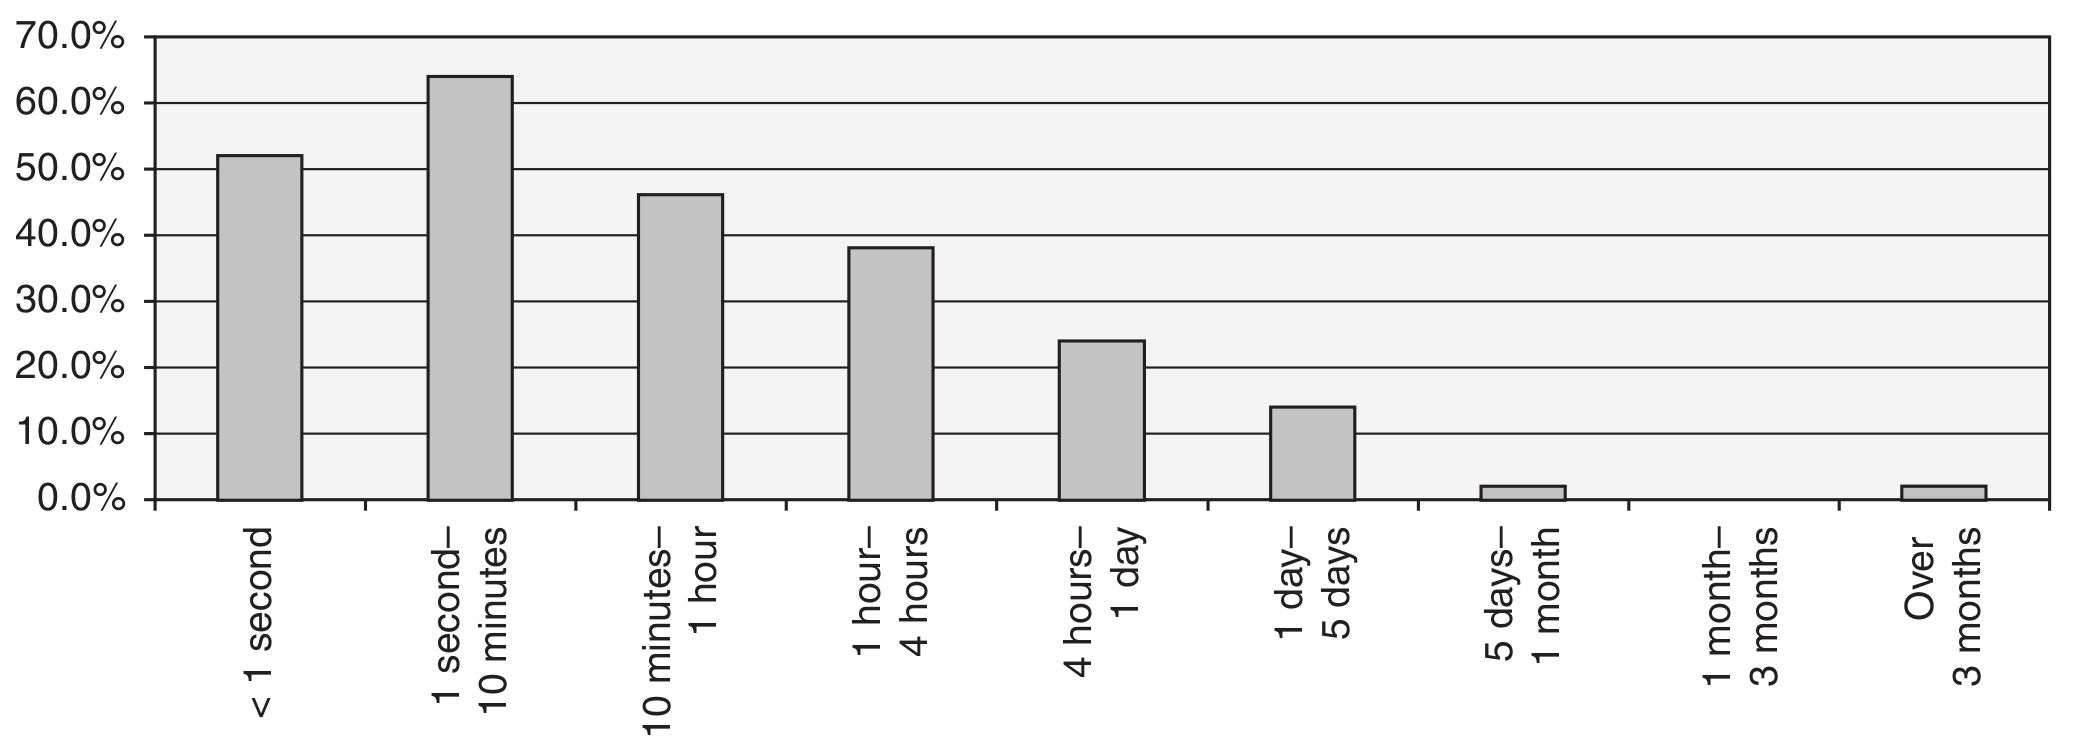
\includegraphics[width=\textwidth]{img/HFTtradestime}
  \caption{Holding time of an opened position of a high frequency trade.Source
  \cite{aldridge2009}.}
  \label{fig:HFTtimes}
\end{figure}
In 2014 HFT represented nearly 50\% of equity trades in the US and more than
20\% in Europe showing a consistent fall since 2009 which was its best year. US
market revenues have fallen dramatically.  Figure~\ref{fig:HFTmarket} on the
left shows HFT trades percentage of US and Europe equity shares. The right
figure shows how revenues in US stocks have fallen the last years.

\begin{figure}[!h]
  %\vspace{-0.8cm}
  \centering
  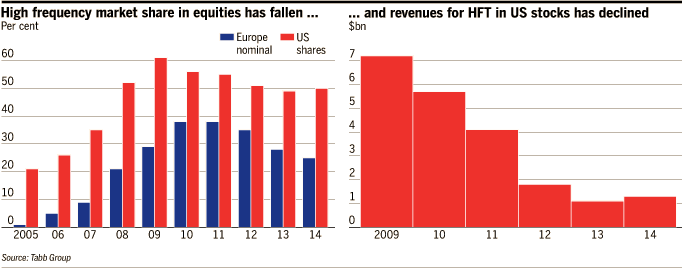
\includegraphics[width=\textwidth]{img/HFTmarket}
  \caption{Left figure shows HFT market share in the US and Europe. Right figure
  shows revenue in the US. Source: TABB Group.}
  \label{fig:HFTmarket}
\end{figure}
One of the reasons of this fall is that exchange markets have adapted, having
now faster, more transparent and efficient market structures than before.
This has been possible due to its investment in technology enhancing
reliability and stability of transactions. Even though this fall, HFT is still a major component of regulated markets and
will probably remain as a topic of interest for researchers in the near future.

On the other hand, HFT has been criticised on qualitative issues concerning
fairness and systemic risk. However, empirical research shows that HFT has lead to
beneficial impacts such as reducing spreads (difference between buyers and
sellers prices), increased liquidity, allowing more efficient price formation,
reduced transaction costs and lower market volatility. HFT makes the stock market more efficient and helps small investors who trade at random times over the day. 


\section{Financial Markets}

A financial market is any marketplace where buyers and sellers participate
trading different assets such as equities, bonds, currencies and derivatives
(future or options). One of the main objectives of financial markets is to set
prices for global trade.
A financial market has many components but the most commonly used are money
markets and capital markets. Money markets are used for short-term basis,
usually for assets up to one year, for greater periods capital markets are used.
Capital markets include the stock or equity market and the bond or debt market
and their movements are the most widely followed \cite{aldridge2009}.

\begin{figure}[!h]
  %\vspace{-0.8cm}
  \centering
  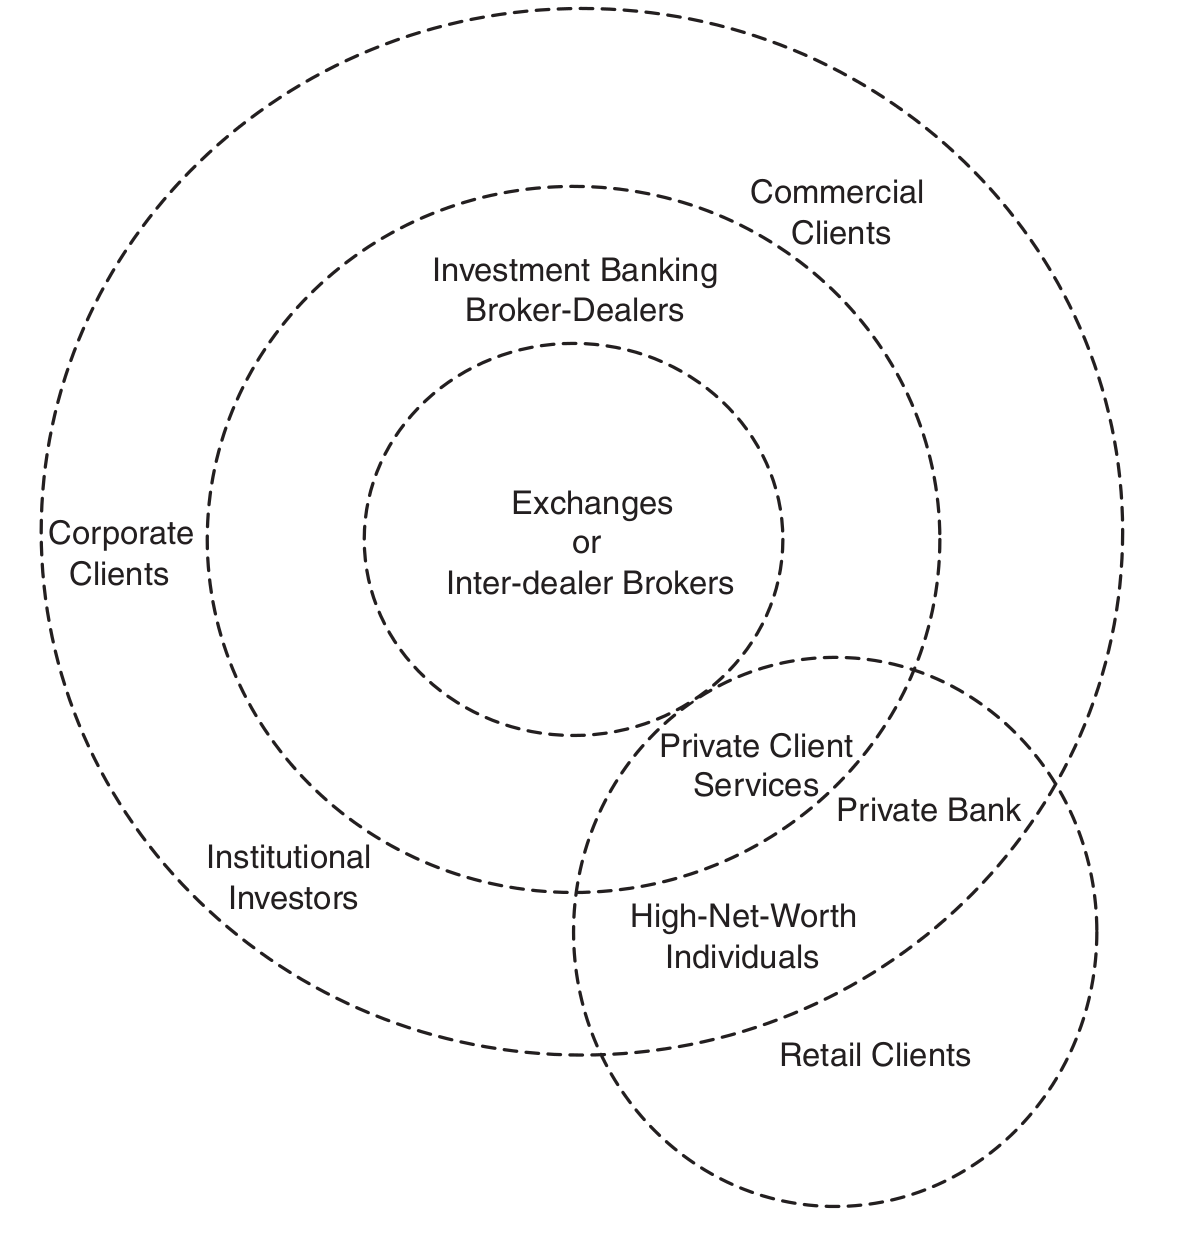
\includegraphics[width=0.7\textwidth]{img/capitalmarkets}
  \caption{Old structure of capital markets. Source \cite{aldridge2009}.}
  \label{fig:capitalmarket}
\end{figure}
Figure~\ref{fig:capitalmarket} shows the typical structure of capital markets
existed from the early 1929s through much of the 1990s where the broker-dealers
played the central and most profitable role.  At the core are the exchanges or
inter-dealer networks (foreign exchange trading). Exchanges are the centralised
marketplaces for transacting.  Broker-dealers perform two functions: trading for
their own accounts and transacting for their customers. Broker-dealers use
inter-dealer brokers to quickly find the best price for a particular asset among
the network of other broker-dealers. Occasionally, broker-dealers also deal
directly with other broker-dealers, particularly for less liquid instruments.
Broker-dealers clients are institutional investors, corporate clients,
commercial clients, and high-net-worth individuals \cite{aldridge2009}.

This centralised structure existed until computer technology allowed a better
communication structure. Today financial markets are more decentralised
providing more liquidity. Exchanges and inter-dealer brokers were replaced by
liquidity pools or Electronic Communication Networks (ECNs) which are able to
transmit order quickly matching buyers and sellers optimally. There are also
dark liquidity pools where trader identity and orders remain anonymous.

Figure~\ref{fig:capitalmarketnow} shows current structure of capital markets
including ECNs and dark pools. In this structure, ECNs, Exchanges, dark pools,
broker-dealers and retail brokerages can execute orders. However, there are some
institutional clients that have also become broke-dealers.

\begin{figure}[!h]
  %\vspace{-0.8cm}
  \centering
  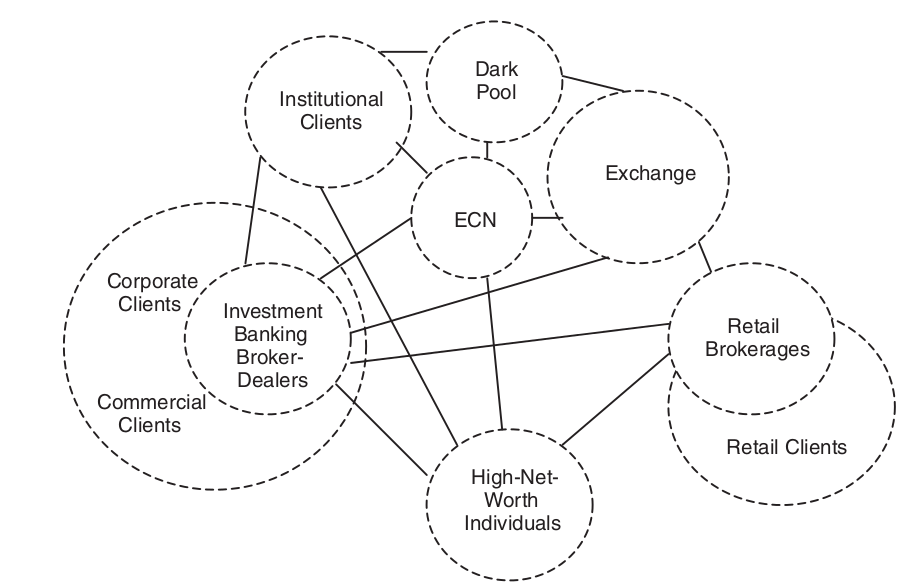
\includegraphics[width=0.8\textwidth]{img/capitalmarketsnow}
  \caption{Actual structure of capital markets. Source \cite{aldridge2009}.}
  \label{fig:capitalmarketnow}
\end{figure}


Equity market and foreign exchange market (Forex) are the most popular markets
for high frequency trading strategies \cite{genccay2001introduction}. In the
Equity market, stocks such as futures and options, exchange-traded funds (ETFs)
among others financial instruments can be traded. Additionally, in the Forex
market, interest rates denominated pair currencies such as EURUSD (Euro to UD
dollar) or USDJPY (US dollar to Japanese yen) are traded. Traders of this
market are diverse, some of them are high frequency traders, long-term
investors and corporations. The Forex market used to be centralised, only
commercial banks had exclusive access to inter-dealer networks. Today, Forex
market is decentralised and has become the biggest market in terms of volume of
trading. The main participants are international banks geographically dispersed
with continuous 24 hours operations excepting weekends.
Figure~\ref{fig:Forextimes} shows different market trading hours in GMT for
London, New York, Sydney and Tokyo.

\begin{figure}[!h]
  %\vspace{-0.8cm}
  \centering
  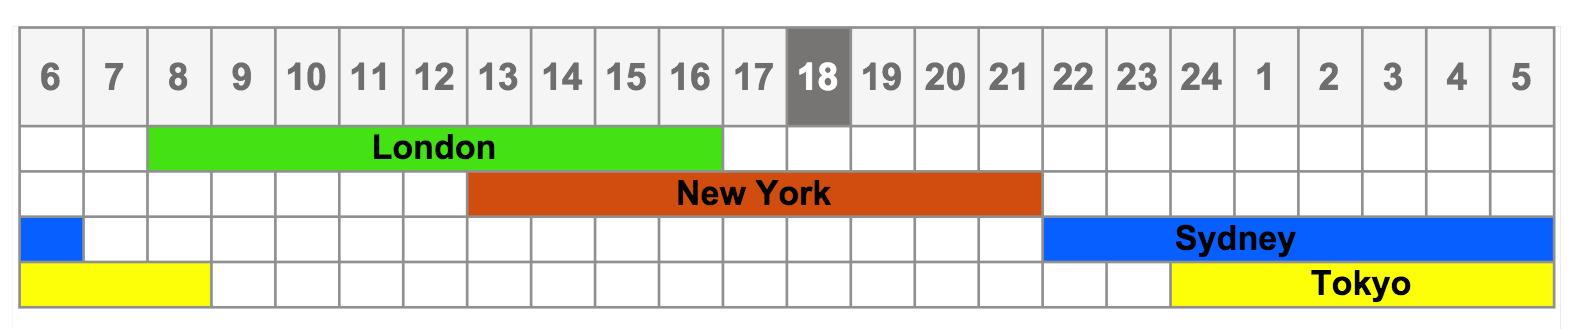
\includegraphics[width=0.8\textwidth]{img/forex-trading-hours.png}
  \caption{Forex market trading hours (GMT). Source \cite{dailyprice}.}
  \label{fig:Forextimes}
\end{figure}


There are three periods of overlaps between different trading times:

\begin{itemize}
\item New York and London from 13:00 GMT until 17:00 GMT
\item Tokyo and London from 8:00 GMT until 9:00 GMT
\item Sydney and Tokyo from 23:00 GMT to 7:00 GMT 
\end{itemize}

These overlap hours are very important since the highest volume of trades are
expected. Therefore, most HFT strategies are executed in these hours.

\section{Price formation process}

A trade consists at least of two orders: one to enter the market (buy order) and
exit the market (sell order). Traders have different types of order they can
execute:

\begin{description}
\item[Market order] allows to buy or sell an asset at the current best price
whatever the price is. The transaction price is determined by the market
considering previous executed orders and volume requested.
\item[Limit order] allow to specify the price you want to buy or sell an asset.
Depending on the market conditions, this type of orders could never been executed.
\item[Stop order] are suitable for investors who are unable to monitor their
investments for a period of time. Stop order allows to specify the price that a
position should be closed; this price is called stop price. When the stop price
is reached a market order is executed, this means that market price could not be
exactly the same specified in the stop order.
\end{description}

In terms of commissions, limit and stop order are more expensive than market orders and
there is no certainty of execution.

Moreover, all orders can specify other parameters such as: 

\begin{description}
\item[Fill or Kill] is an order that must be executed immediately or being
cancelled, no partial fulfillments are allowed. 
\item[Day] the order is only valid during the day.
\item[Good til canceled] a order is active until the investor decides to cancel
it or the trade is executed.
\end{description}

In order to determine the execution price, buyers and sellers orders are placed
in an order book which help to determine which order can be fulfilled.
Figure~\ref{fig:orderbook} illustrates how buyers and sellers are ordered. The
ask or offer price is the current lower price a seller is willing to accept for
a good. The bid price corresponds to the current highest price a buyer is
willing to pay for a good. Orders with the same price are prioritised by
arrival time and placed on top of the book.  The difference between current ask
and bid price is called spread and their average is called mid-price
\cite{bouchaud2002statistical}.

\begin{figure}[!h]
  %\vspace{-0.8cm}
  \centering
  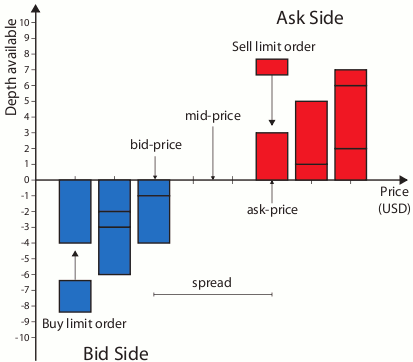
\includegraphics[width=0.5\textwidth]{img/orderbook}
  \caption{Order book. Buyers and sellers are ordered according to the bid or
ask price and the market determines the mid-price and transacted volume. Source
\cite{gould2013limit}.}
  \label{fig:orderbook}
\end{figure}
Today, order books are available and they are a popular source of study among
researchers. The mid-price and spread modelling are some of the
problems related with this area. 


\section{Efficient market hypothesis}

Efficient Market Hypothesis (EMH) was developed independently by  Paul
Samuelson and Eugene Fama in the 1960s.  EMH also known as the random walk
theory states that current stock prices fully reflect available information
related to its value and there is no way to earn excess profits
\cite{fama1970}. EMH requires that all the participants have rational
expectations, and investors reactions be random and follow a normal
distribution pattern. Thus, any one can be wrong about the market, but the
market is always right as a whole.  There are three common forms of EMH:
weak-form efficiency, semi-strong efficiency and strong-form efficiency.

The weak form claims that prices already reflect all past publicly available
information. Therefore, future prices cannot be predicted based on analysis of
historical data. This implies that future prices movements are determined
entirely by information not contained in the past prices and participants are
unable to systematically profit from market inefficiencies.  However, many
studies have shown a marked tendency for the stock markets to trend over time
periods. Various explanations for such large and apparently non-random price
movements have been promulgated. Even Fama has accepted price anomalies which
do not follow the weak-form efficiency hypothesis \cite{fama+french2008}.

The semi-strong form of the EMH claims that prices instantly change to reflect
new public (not private) information such that no excess return can be
obtained. 

The strong form of the EMH additionally claims that prices instantly reflect
even hidden, private or ``insider" information. 

EMH is related with two approaches to investment analysis: fundamental and
technical analysis. Fundamental analysts base their predictions of stock price
behaviour on fundamental factors such as internal information of a company, its
industry or the economy. Technical analysts, by contrast, consider that all
this financial information is already included in the prices and believe that
future stock prices can be predicted studying the historical market behaviour.
A market technician bases his predictions on historical patterns of prices of
volume changes.

Under the weak form of EMH, strategies based on technical analysis will not be
able to produce excess returns. However, the weak form accepts that some forms
of fundamental analysis may still provide excess return. Similarly, the
semi-strong form of EMH  neither technical or fundamental analysis can produce
excess return.

If the stock market efficiently digests all available information, there is
little justification for seeking excess returns gains from investing. However,
EMH doesn't lessen the importance of investing only change its philosophy. The
only way an investor can possibly obtain higher returns is by purchasing
riskier investments.

 Researches can determine now how efficient a financial market is, i.e how
efficiently information is processed.  

EMH is based on rational human behaviour and its validity has been criticised
by psychologists and behavioural economists who argue that the EMH is based on
counterfactual assumptions regarding human behaviour, that is, rationality.
Recent advances in evolutionary psychology and the cognitive neurosciences may
be able to reconcile the EMH with behavioural anomalies. On the other hand, if
the EMH is true, the market really walks randomly and therefore there shouldn't
be any difference between experienced and novice traders. Kim Man Lui proved
the contrary in a controlled experiment \cite{man2013}.



\chapter{Financial Time Series}

\vspace{0.5cm} 
 
A time series is a collection of observations in time (discrete or continuous).
The analysis of time series main objective is to find possible internal
structure in the data such as autocorrelation, trend or seasonal variation.
Some of application and uses of time series analysis are data compression,
explanatory variables (relationships with other variables, seasonal factors,
etc.), signal processing and forecasting (predict future values), which is the focus of this thesis. 
There are two main approaches to study financial time series: to study directions of financial
rates and to explain financial rate volatility.  This chapter reviews the most
relevant techniques in the rich and rapidly growing field of time series
analysis considering these two approaches.


\section{Characteristics of Financial Time Series}
%\section{Stylized facts of asset returns}
\label{sec:stylizedfacts}

There are several known features exhibited by financial instruments called
stylized facts, which have been empirically studied and some of them have been
documented only recently and accepted as truth. Stylized facts are usually
formulated in terms of qualitative properties of asset returns and may not be
precise enough to distinguish among different parametric models.
\cite{cont2001}.

Returns of a time series $y_t$ is defined as:
\begin{equation}
\label{eq:returndef}
r_t = y_t - y_{t-1}  \, ,
\end{equation}

Some stylized facts which are common to a wide set of financial assets
\cite{sewell2011} are:

\begin{description}
\item[Dependence] autocorrelation function (ACF) in returns is largely insignificant. The ACF measures the linear predictability of the series at time $t$ using only the value at time $s$:

\begin{equation}
\rho(s,t) = \frac{\gamma(s,t)}{\sqrt{\gamma(s,s)\gamma(t,t)}}
\end{equation}
\noindent where $\gamma(s,t)$ is the autocovariance function measures the linear dependence between two points on the same series observed at different times, it is defined as the second moment product:
\begin{equation}
\gamma_y(s,t) = E[(y_s-\mu_s)(y_t - \mu_t)]
\end{equation}
However, the autocorrelation in the absolute and squared returns is always positive,
significant and decays slowly. In addition, the autocorrelation in the absolute
returns is generally higher than the autocorrelation in the corresponding
squared returns. The returns autocorrelation function (ACF) of SPY is shown in figure
 \ref{fig:returnacf}. The figure shows how the correlations are significant even
 for very long lags, this imply that a long-memory process because of its
 long-range dependence. 
 \begin{figure}[h]
 \centering
 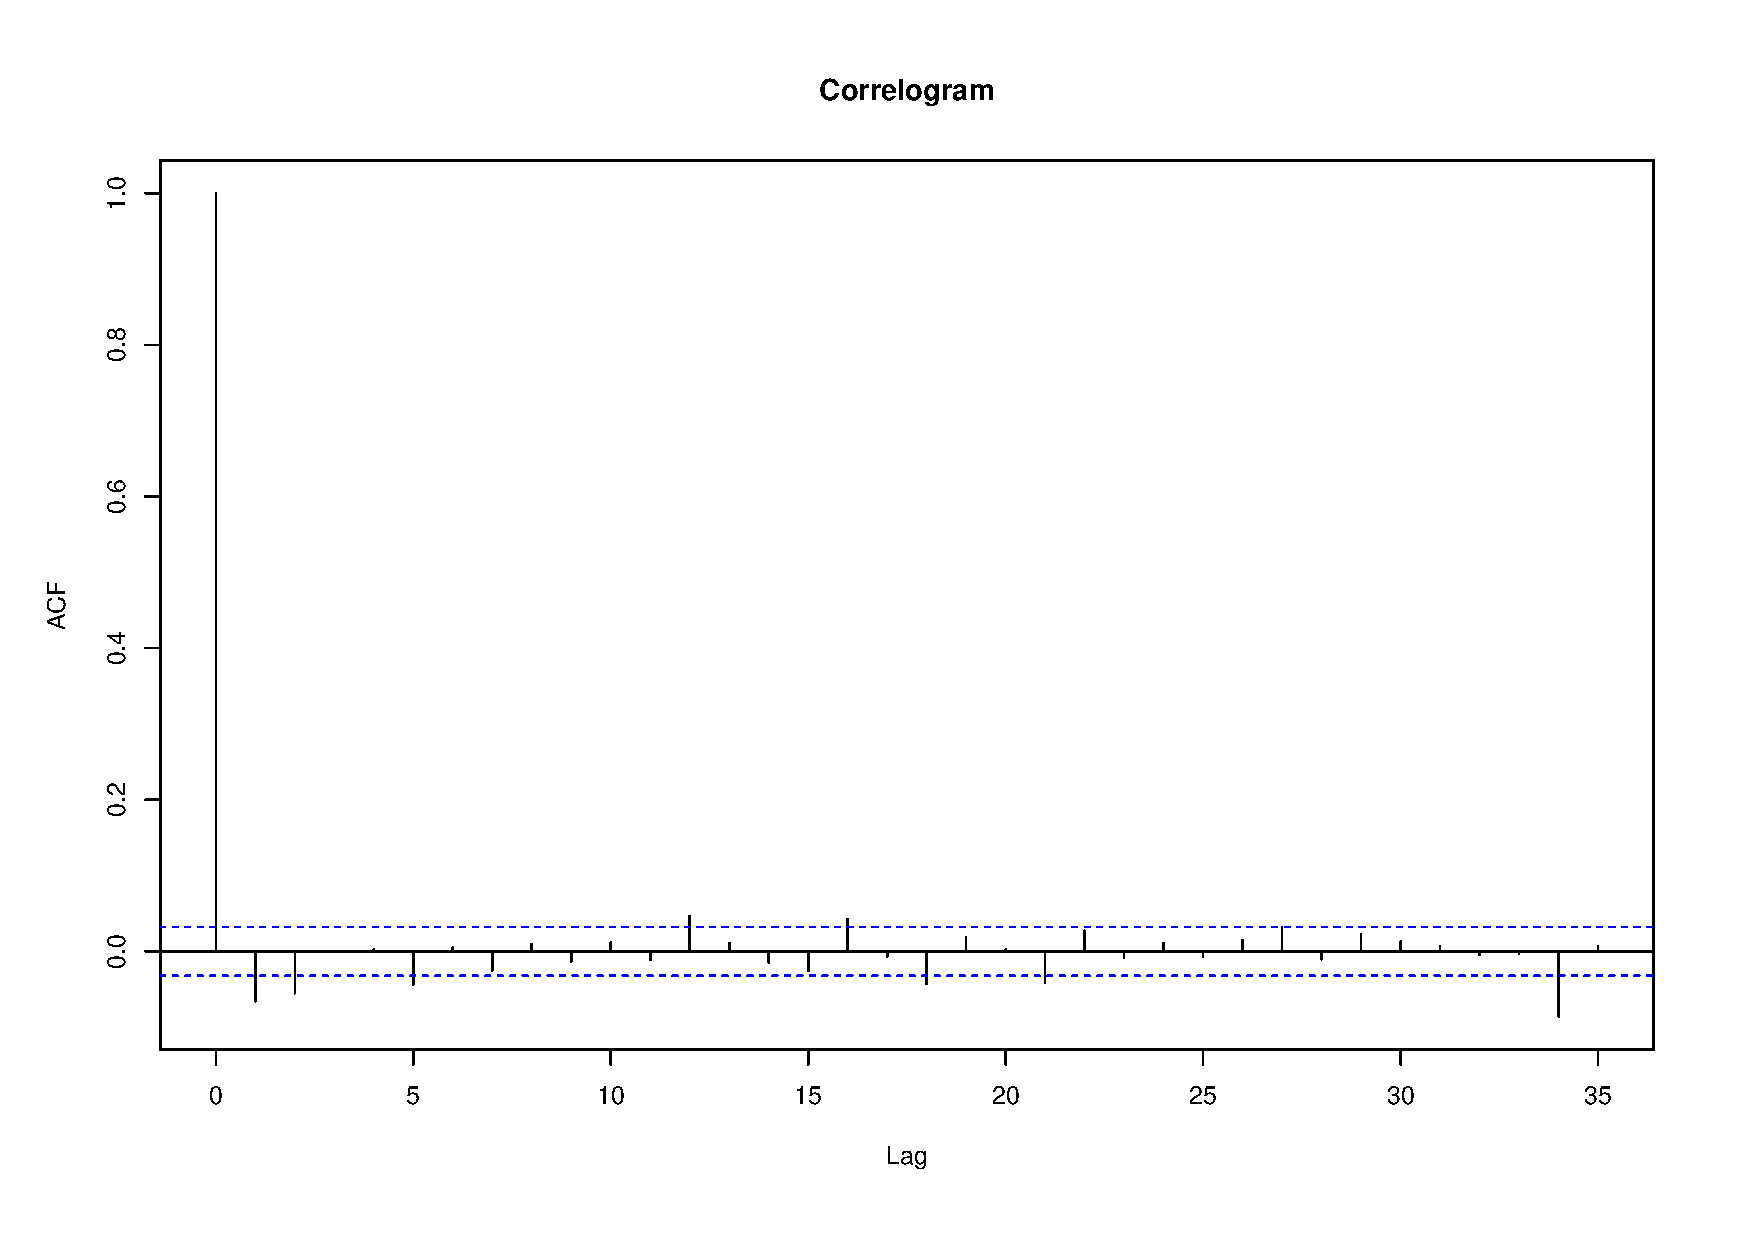
\includegraphics[width=0.7\textwidth]{plots/spy_returns_acf.pdf}
 \caption{SPY returns ACF}
 \label{fig:returnacf}
\end{figure}
\item[Distribution] The distribution of returns is approximately symmetric and
has high kurtosis (i.e fat tails and a peaked centre compared with the normal
distribution). However, distribution of returns whose were obtained from higher
frequencies looks more like a normal distribution.
The returns distribution tails are larger than
 what is hypothesised by common data generation process (generally normal
 distribution assumption). In the markets, fat tails are an undesirable feature
 because of the additional risk they imply.  In the figure \ref{fig:returndist}
 is shown the SPY returns distribution based on daily dates from the period 1st
 July 1998 to 4th April 2013. The distribution was compared against the normal
 distribution which clearly doesn't fit the data.  
 \begin{figure}[h]
 \centering
 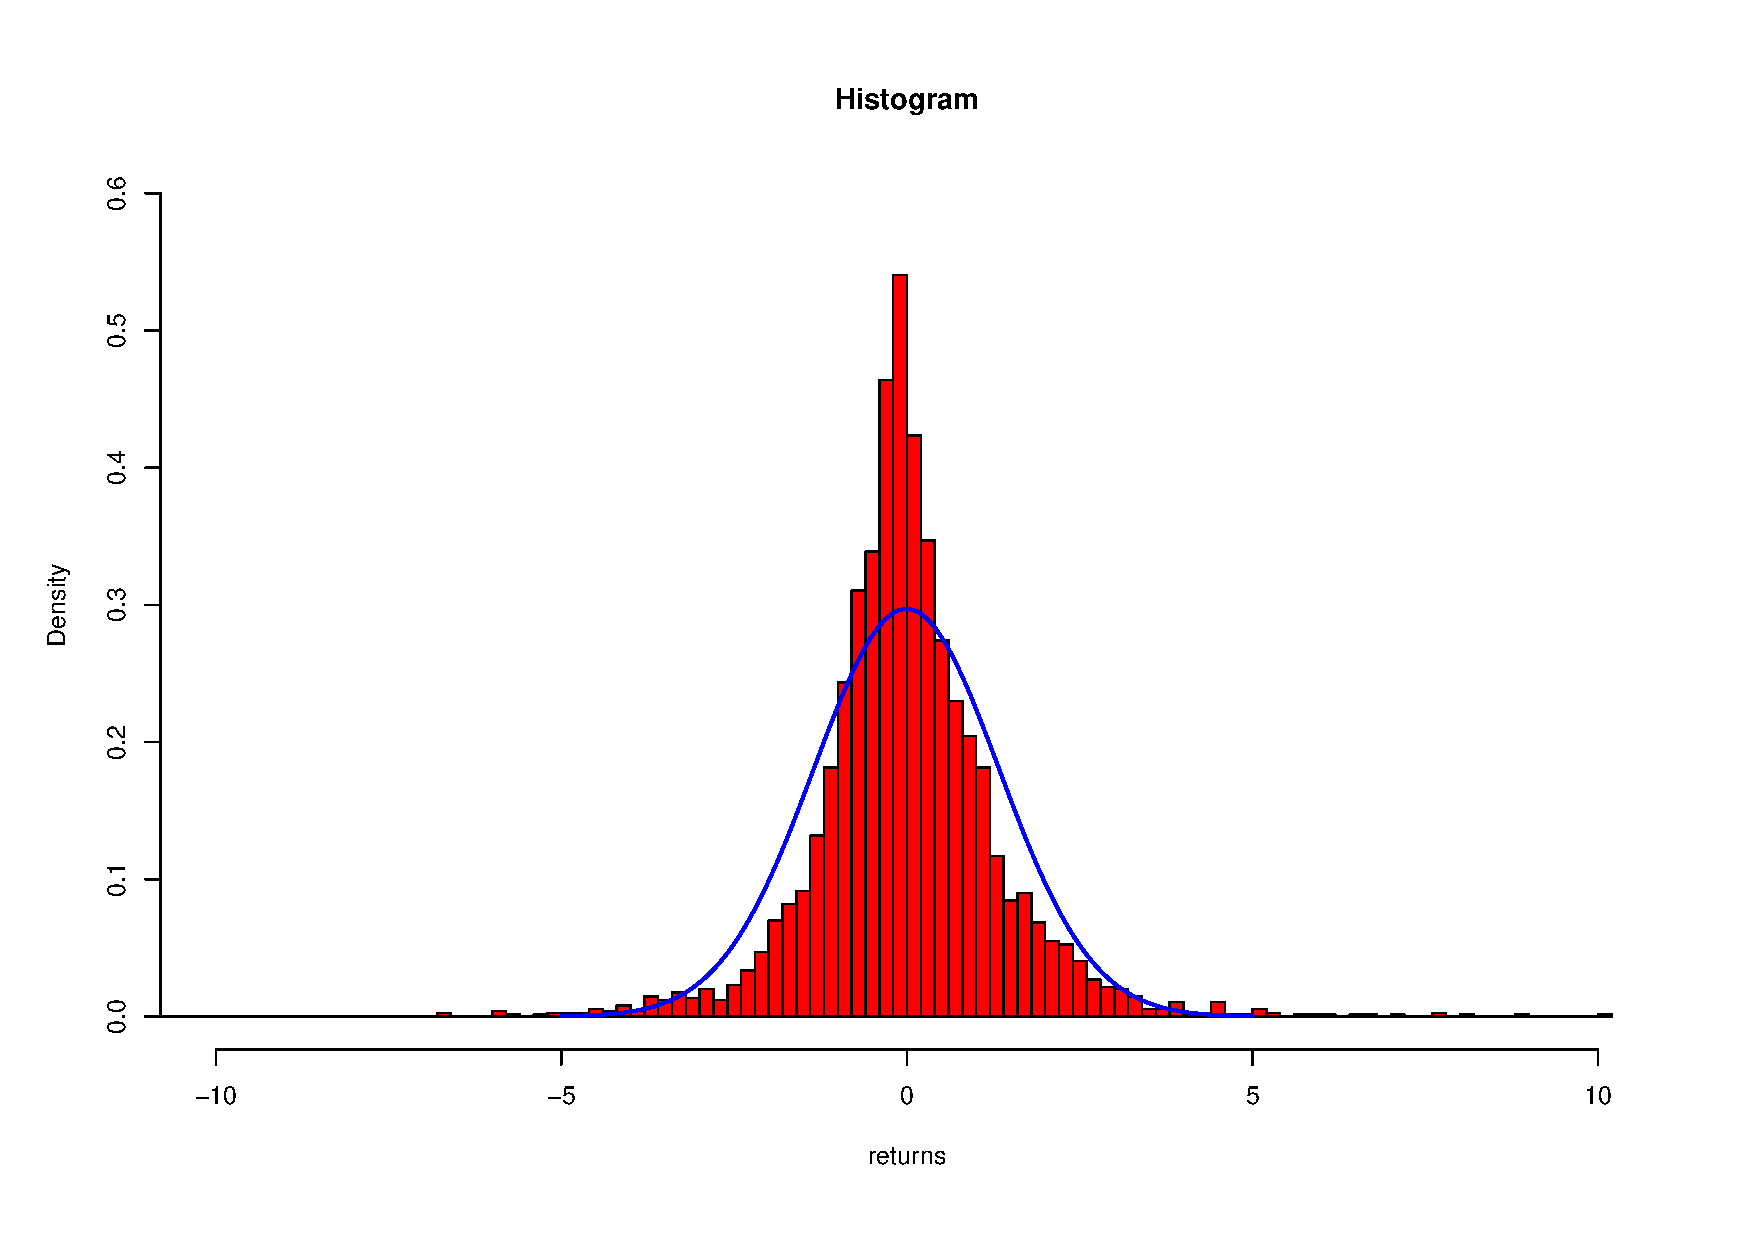
\includegraphics[scale=0.5]{plots/spy_returns_dist.pdf}
 % spy_returns_dist.pdf: 504x504 pixel, 72dpi, 17.78x17.78 cm, bb=0 0 504 504
 \caption{SPY returns distribution}
 \label{fig:returndist}
\end{figure}
\item[Heterogeneity] despite the fact that financial returns are non-stationary,
stationary periods can be observed. Economist speaks in terms of a structural
break \cite{stock1994}, in machine learning this is known as drift which means
that the statistical properties of the target variable change over time
\cite{widmer1996}, \cite{tsymbal2004}.
\item[Non-Linearity] financial returns may be non-linear in mean and/or
non-linear in variance.
\item[Calendar effects] are also called seasonal effects and they are cyclical
anomalies in returns where the cycle is based on the calendar. Some of known
calendar effects are: intraday effect, weekend effect, Monday effect, intramonth
effect, the January effect and Holiday effect. The most important calendar
anomalies are the January effect and the weekend effect. Figure
\ref{fig:mondayeffect} shows the Monday effect from 1928 to 2007. It shows that
in average Monday has negative returns. However, this is changing in time,
figure \ref{fig:mondayeffect2} shows returns only for year 2007 and its last
three months and it shows that Mondays and Wednesdays has positive returns in
average.

\begin{figure}[h!]
\centering
\begin{subfigure}[b]{0.45\textwidth}
 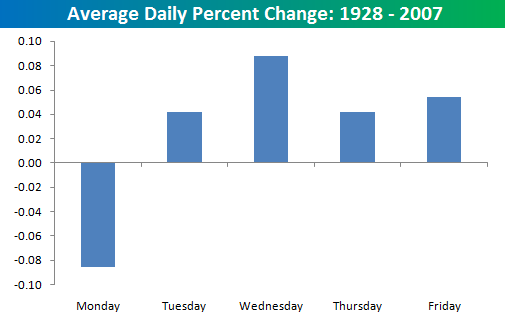
\includegraphics[width=\textwidth]{img/average_daily_change_1928_2007}
 \caption{Average daily return: 1928-2007}
 \label{fig:mondayeffect}
\end{subfigure}
\begin{subfigure}[b]{0.45\textwidth}
 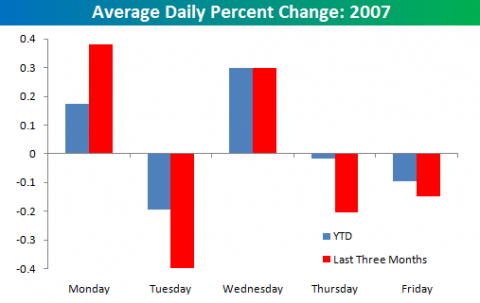
\includegraphics[width=\textwidth]{img/thumb-average_daily_change_2007}
 \caption{Average daily return: 2007}
 \label{fig:mondayeffect2}
\end{subfigure}
\end{figure}
\end{description}


\subsection{Stationary }
A strictly stationary times series $Y_t$ is one for which the probabilistic behaviour
of every collection of values $\{Y_{t_1},Y_{t_2},\dots,Y_{t_L}\}$ is identical
to that of the time shifted set, more precisely: \[ P\{Y_{t_1} \leq
c_1,\dots,Y_{t_L} \leq c_L\} = P\{Y_{t_1+h} \leq c_1,\dots,Y_{t_L+h} \leq c_L\}
\quad \forall L \in \mathbb{N}, \forall h \in \mathbb{Z}\] \noindent where
$c_1,\dots,c_L$ are constants.  This definition is too strong and difficult to
assess it from a single data set. The weak version of this definition imposes
conditions only on the two first two moments.

A weakly stationary time series is a process which mean, variance and auto
covariance do not change over time: \begin{eqnarray*} E(Y_t) &=& \mu  \quad
\forall t \in \mathbb{N} \\ E(Y^2_t) &=& \sigma^2  \quad \forall t \in
\mathbb{N} \\ \lambda(s,t)&=&\lambda(s+h,t+h) \quad \forall s,t \in \mathbb{N},
\forall h \in \mathbb{Z} \end{eqnarray*}

\noindent with $\lambda(s,t) = E[(Y_s-\mu)(Y_t - \mu)]$ 

In finance, a shock represents an unexpected change in a variable or a in its
error term in a particular time period. For stationary time series, shocks to
the system will gradually die away. That is, a shock during time $t$ will have a
smaller effect in time $t+1$, a smaller effect on $t+2$ and so on. For
non-stationary data, the persistence of shocks will always be infinite. 

\subsection{Non-stationary processes}

There are different types of non-stationary time series models often found in economics:


\subsubsection{Deterministic trend}

Deterministic trend or trend stationary processes have the following form:

\[
X_t = f(t) + \epsilon{t} \quad ,
\]

\noindent where $t$ is the time trend and $\epsilon{t}$ represents a stationary error term (with mean 0 and variance $\sigma^2$) and $f(t)$ is a deterministic function of time:
\begin{itemize}
\item If $f(t) = \alpha + \beta t$ we have a linear trend model which is widely used. 
\item If $f(t)= \alpha \exp^rt$ we have an exponential growth curve.
\item If $f(t) = c_1 + c_2t + c_3 t^2$ we have a quadratic trend model
\item If $f(t) = \frac{1}{k+\alpha \beta ^t }$ we have a logistic curve
\end{itemize}

\subsubsection{Stochastic trend}
Stochastic trend processes are also called unit root or difference stationarity processes and have the following form:

\[
X_t = \mu + X_{t-1} + \epsilon_t
\]
\noindent where $\epsilon_t$ is a stationary process. When $\mu = 0 $ the process is called pure random walk and when $\mu \neq 0$  the process is called random walk with drift.

Alternatively this process can be expressed using the lag operator $L$ such as:

\[
(1-L) X_t = \mu  + \epsilon_t
\]

This process is also called unit root because the root of the characteristic equation ($1-z = 0$) is the unity.  

A random walk with or without drift can be transformed to a stationary process by differencing the time serie once. The disadvantage of differencing is that the process loses one observation each time the time series is differentiated.

Apart from a stochastic trend, many economic financial time series seem to involve an exponential trend, this is the reason why researchers often take the logarithmic transformation before doing analysis.

Other less common forms of non-stationarity are structural break in mean and structural break in variance. 

\newpage
\subsection{Spurious regression} \label{sec:spurious}
The use
of non-stationary data can lead to spurious regressions. Spurious regression
dates back to Yule in 1926 \cite{yule1926} If two stationary
variables are generated as independent random series and are trending over time,
when one of those variables is regressed on the other, they could have a high
$R^2$ even if the two are totally unrelated. So, if standard regression
techniques are applied to non-stationary data, it could look good under standard
measures but valueless \cite{brooks2002}.

\textbf{Example of spurious regression} \quad 
An example is shown below. Two random walks series $x_1t$ and $x_2t$ with a small drift ($\alpha=0.09$) are generated and
then regressed one on the other:
 \begin{equation}
 x_i,t = \alpha + x_{i,t-1} + \epsilon_i,t  \qquad \text{where} \qquad \mathcal{N}(0,1), \quad i=1,2
 \end{equation}

\begin{figure}[!h]
  \centering
  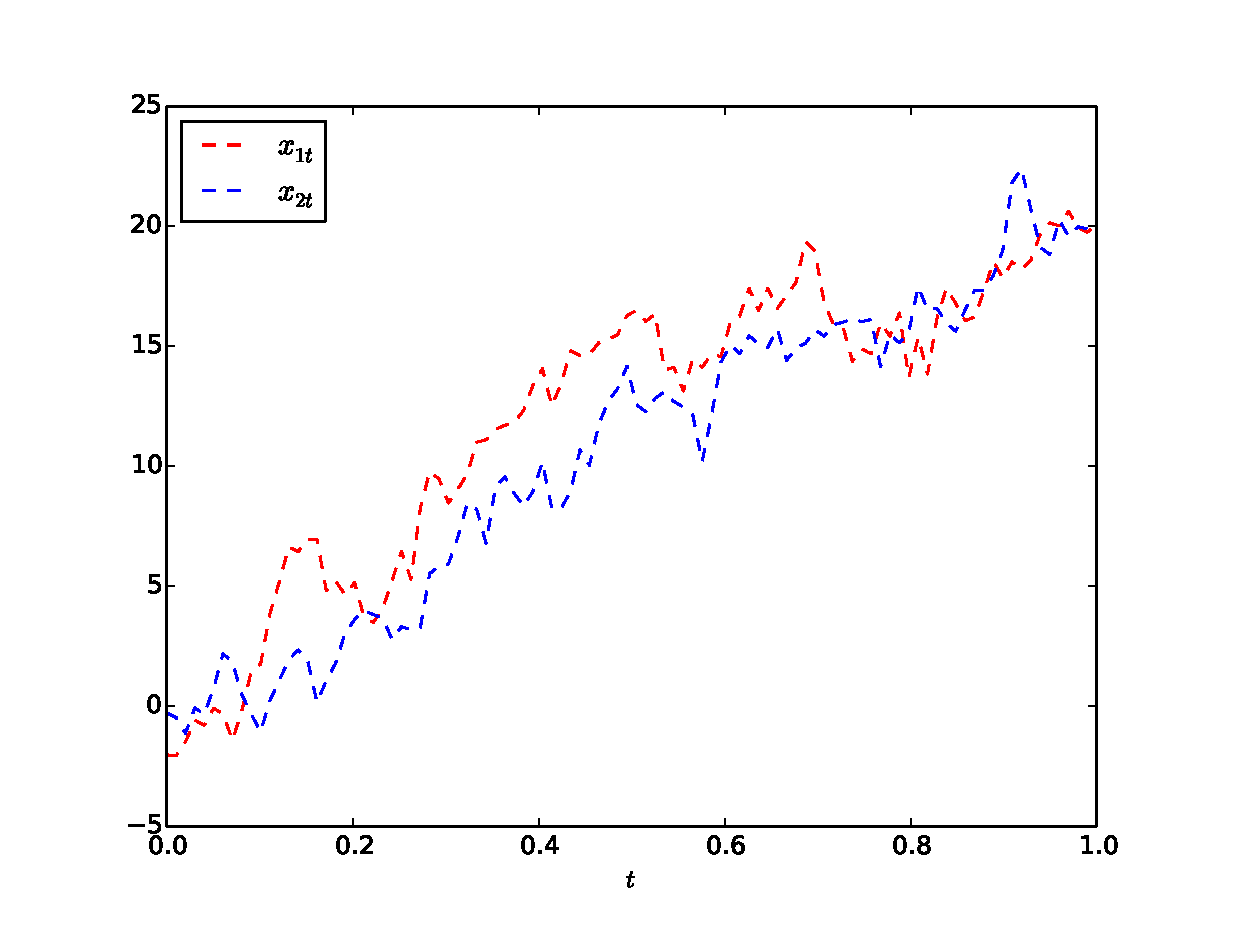
\includegraphics[width=0.8\textwidth]{img/spurious1}
  \caption{Two random walks time series $x_1,t$ and $x_2,t$}
  \label{fig:spurious1}
\end{figure}

\begin{figure}[!h]
  \centering
  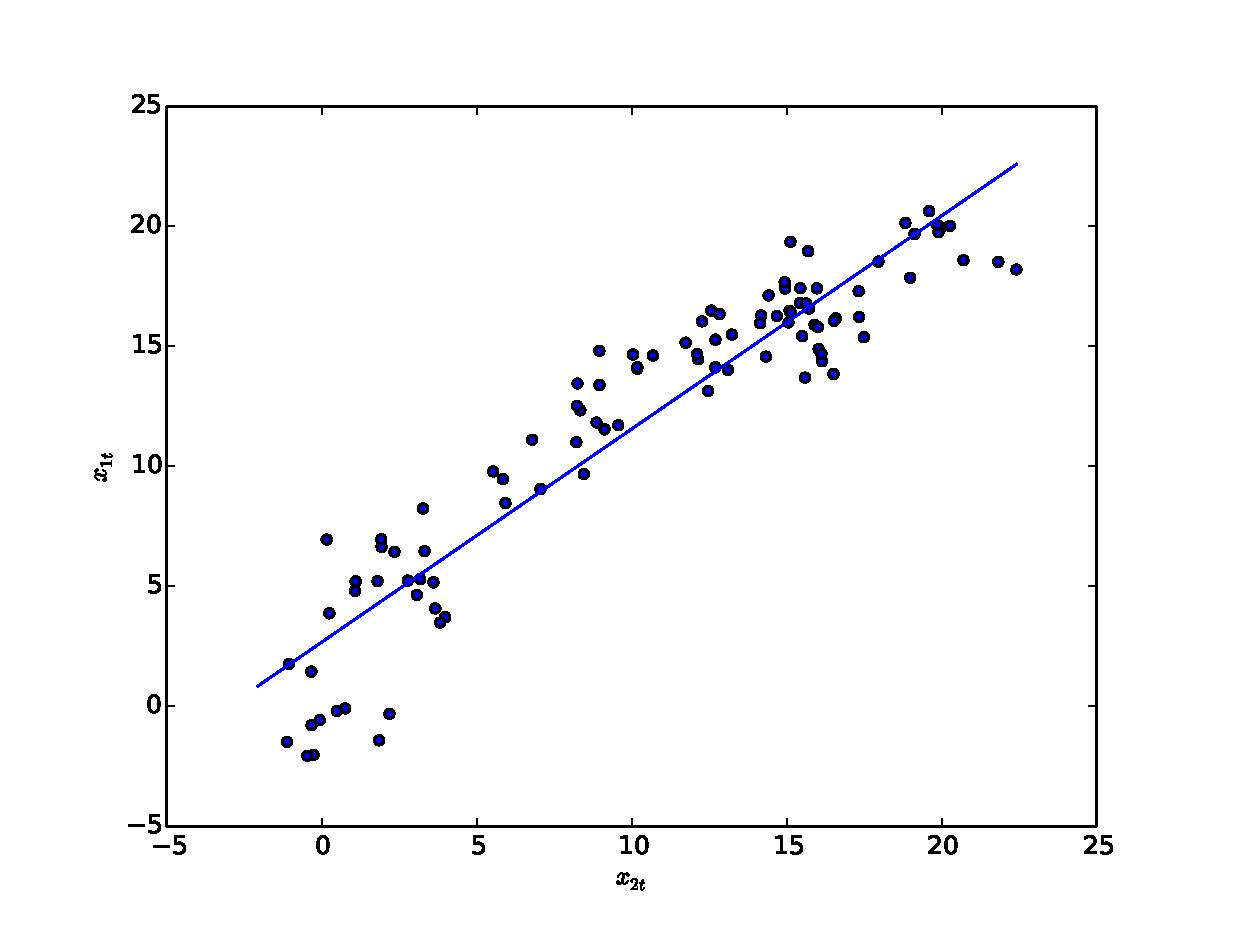
\includegraphics[width=0.8\textwidth]{img/spurious2}
  \caption{Regression between two random walks time series}
  \label{fig:spurious2}
\end{figure}

These two random walks, which are independent by construction, appear to be related with a $R^2=0.883$. However, what it is happening is that they are drifting in the same direction. Drift can be removed using returns or first differences.
If after taking returns or first differences the regression fit is still good we will say that the variables are cointegrated, this means that both series may drift but their residuals will not. A more formal definition of cointegration is given in the section \ref{sec:cointegration}.

%                            OLS Regression Results                            
%==============================================================================
%Dep. Variable:                      y   R-squared:                       0.883
%Model:                            OLS   Adj. R-squared:                  0.882
%Method:                 Least Squares   F-statistic:                     742.2
%Date:                Fri, 06 Feb 2015   Prob (F-statistic):           1.61e-47
%Time:                        06:07:47   Log-Likelihood:                -218.03
%No. Observations:                 100   AIC:                             440.1
%Df Residuals:                      98   BIC:                             445.3
%Df Model:                           1                                         
%==============================================================================
%                 coef    std err          t      P>|t|      [95.0% Conf. Int.]
%------------------------------------------------------------------------------
%x1             0.8883      0.033     27.243      0.000         0.824     0.953
%const          2.6726      0.405      6.606      0.000         1.870     3.475
%==============================================================================
%Omnibus:                        4.133   Durbin-Watson:                   0.363
%Prob(Omnibus):                  0.127   Jarque-Bera (JB):                4.145
%Skew:                          -0.469   Prob(JB):                        0.126
%Kurtosis:                       2.662   Cond. No.                         23.3
%==============================================================================
$\blacksquare$

\newpage
\subsection{Integration}

Following Johansen \cite{johansen1995} we shall say that a stochastic process
$Y_t$ which satisfies $Y_t-E(Y_t) = \sum_{i=0}^\infty C_i\,\varepsilon_{t-i}$ is
called $I(0)$, and then we shall write $Y_t\sim I(0)$, whenever
$\sum_{i=0}^\infty C_i \neq 0$ and $\sum_{i=0}^\infty C_i\,z^i$ converges for
$z\in\mathbb{C}$ with $|z|<1$.  It is understood that the condition
$\varepsilon_t\sim iid(0,\sigma^2)$ holds.

A (vector) time series $\mathbf{y}_t$ is said to be {\em integrated of order\/}
$d$, and then we shall write $\mathbf{y}_t\sim I(d)$, whenever after $d$ times
(discrete) differentiation an stationary process is
obtained~\cite{banerjee1993};
more precisely, whenever
$(1-L)^d\,\mathbf{y}_t\sim\text{I(0)}$, where $L$ is the usual lag operator:
$(1-L)\,\mathbf{y}_t = \Delta\mathbf{y}_t = \mathbf{y}_t-\mathbf{y}_{t-1}$ for
all $t$.  

Note that this definition includes the scalar case as time series of
vectors of dimension 1; in this scalar case we will write the time series in
non-bold format.


\subsection{Cointegration} \label{sec:coint}
Cointegration concept was introduced by Engle in 1987 \cite{engle1987} and implies that one or
more linear combinations of non-stationary variables are stationary even though
individually they are not.  

Let $\mathbf{y}_t^\nu$, $\nu=1,\dots,p$, be a set of $p$ vector time series of
order $I(1)$.  They are said to be {\em cointegrated\/} if a vector
$\beta=[\beta(1),\dots,\beta(p)]^\top \in \mathbb{R}^p$ exists, such that the
time series,
\begin{equation}
\mathbf{Z}_t:= 
\sum_{\nu=1}^p \beta(\nu)\,\mathbf{y}_t^\nu\,\sim\,\text{I(0)}\,.
\end{equation}

In other words, a set of $I(1)$ time series is said to be cointegrated if a
linear combination of them exists, which is I(0).

Stock and Watson in 1988 \cite{stock+watson1988} observed that
cointegration reflects the common stochastic trends providing a useful way to
understand cointegration relationships. These common stochastic trends can be
also interpreted as a long-run equilibrium relationships.

The idea of cointegration was immediately adopted in finance since it could
represent their long-run relationship implied by economic
theory~\cite{laietAl1991}, \cite{lence+falk2005}.  Economic theory suggest that
economic time series are mean-reverting process and therefore, it reflects the
idea of that some set of variables cannot wander too far from each other. 

On the other hand, the efficient markets hypothesis, also known as the random
walk theory states that current stock prices fully reflect available information
related to its value and there is no way to earn excess profits~\cite{fama1970}.
This means that if we have stock prices from a jointly efficient market, they
cannot be cointegrated \cite{granger1986}, \cite{dwyer1992}. However,
\cite{richards1995} claims that cointegration is directly at odds with market
efficiency, even though, there is no evidence that cointegration among asset
prices have implications about market efficiency~\cite{lence+falk2005}.

Despite the fact that cointegration on closing daily rates of currency pairs has
not been found \cite{coleman1990}, \cite{copeland1991}, different time series
frequencies can have different behaviours~\cite{aldridge2009}. Pair trading is a
very common example of cointegration application~\cite{herlemont2003} but
cointegration can also be extended to a larger set of
variables~\cite{mukherjee1995},\cite{engle2004}.

\subsection{Johansen method}
Johansen in 1988 \cite{johansen1988} suggests a method for determining cointegration vectors. 

There are two statistics for cointegration under Johansen approach: the trace (shown in equation \ref{eq:johansentrace}) and the maximum-eigenvalue statistic (shown in equation \ref{eq:johansenmax}).

\begin{equation}
\label{eq:johansentrace}
\lambda_{\text{trace}} (r) = -T \sum_{i=r+1}^g \ln(1-\hat{\lambda_i})
\end{equation}


\begin{equation}
\label{eq:johansenmax}
\lambda_{\text{max}} (r,r+1) = -T \ln(1-\hat{\lambda_{r+1}})
\end{equation}


Where $r$ is the number of cointegration vectors and $\hat]{\lambda}_i$ is the estimated value for the ith ordered eigenvalue.  $\lambda_{\text{trace}}$ null hypothesis is that the number of cointegration vectors is less than or equal to $r$ against that there are more than $r$. $\lambda_{\text{max}}$ has the null hypothesis that the number of cointegration vectors is $r$ against an alternative of $r
+1$.


\newpage
\textbf{Cointegration example} \quad

If we have two-dimensional process $\mathbf{X}_t$, $t=1,\dots,T$ by:

\begin{eqnarray*}
\mathbf{X}_{1t} &=& \sum_{i=1}^t \epsilon_{1i} + \epsilon_{2t} \\
\mathbf{X}_{2t} &=& a \sum_{i=1}^t \epsilon_{1i} + \epsilon_{3t} 
\end{eqnarray*}

Since $\mathbf{X}_{1t}$ and $\mathbf{X}_{2t}$ are I(1) processes and there
exist a vector $\beta = [a -1]$ such that:

\[
\beta^\top \mathbf{X}_t = a \mathbf{X}_{1t} -\mathbf{X}_{2t} = 
a\epsilon_{2t} - \epsilon_{3t} \sim \text{I(0)}
\]

then, both processes are said to be cointegrated. 


If we add a I(0) process
$\mathbf{X}_{3t} = \epsilon_{4t}$  we find that there exists two cointegration
vectors now: $\begin{bmatrix}a &-1& 0\end{bmatrix}$ and $\begin{bmatrix}0
&0&1\end{bmatrix}$ since:

\[
\beta^\top \mathbf{X}_t = 
\begin{bmatrix}
a & -1 & 0 \\
0 & 0 & 1
\end{bmatrix} 
\begin{bmatrix} 
\mathbf{X}_{1t} \\
\mathbf{X}_{2t} \\
\mathbf{X}_{3t}
\end{bmatrix} = 
\begin{bmatrix}
a\epsilon_{2t} - \epsilon_{3t} \\
\epsilon_{4t}
\end{bmatrix}
\]



\begin{figure}[!h]
  \centering
  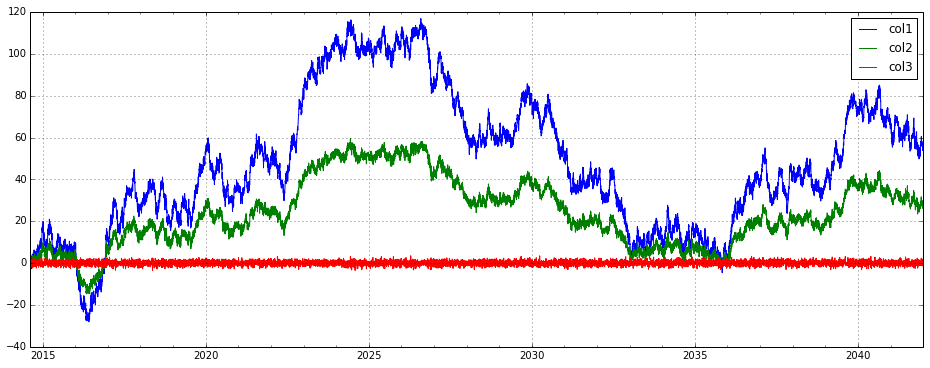
\includegraphics[width=\textwidth]{img/coint-example}
  \caption{Cointegration example: two processes I(1)(blue and green) and one process I(0) (red)}
  \label{fig:cointex}
\end{figure}

\begin{figure}[!h]
  \centering
 \begin{minipage}{\textwidth} %[b][\textheight][s]
  \centering
  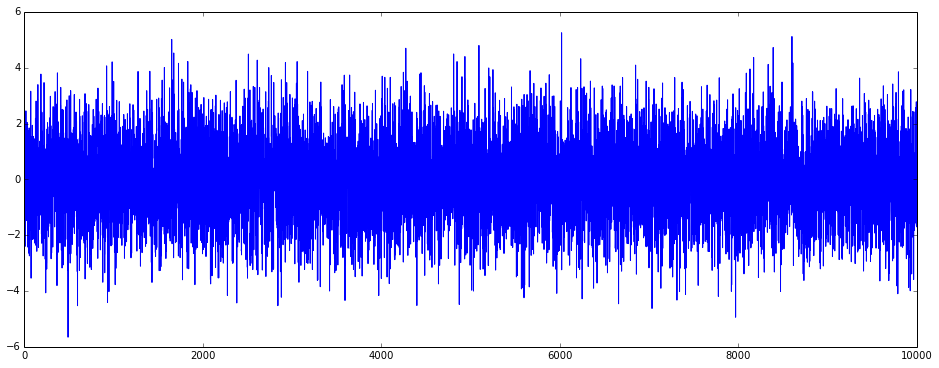
\includegraphics[width=0.9\textwidth]{img/coint-example2} 
   \caption{Time series linear combination using the first cointegration vector }
    \label{fig:cointvectors3}
   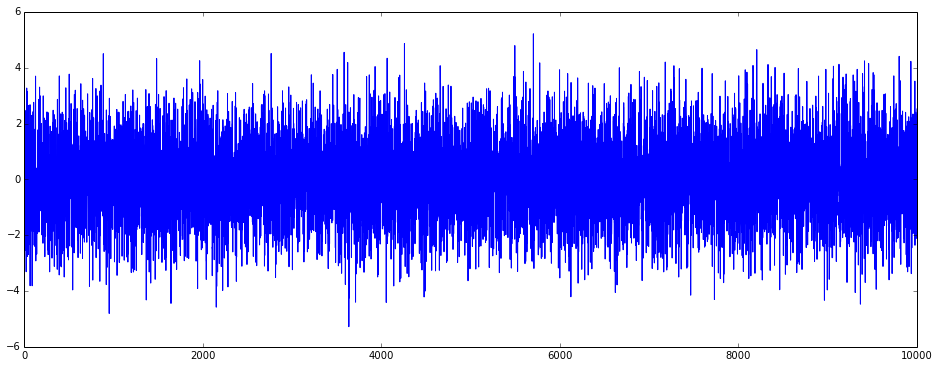
\includegraphics[width=0.9\textwidth]{img/coint-example3} 
    \caption{Time series linear combination using the second cointegration vector}
     \label{fig:cointvectors4}
    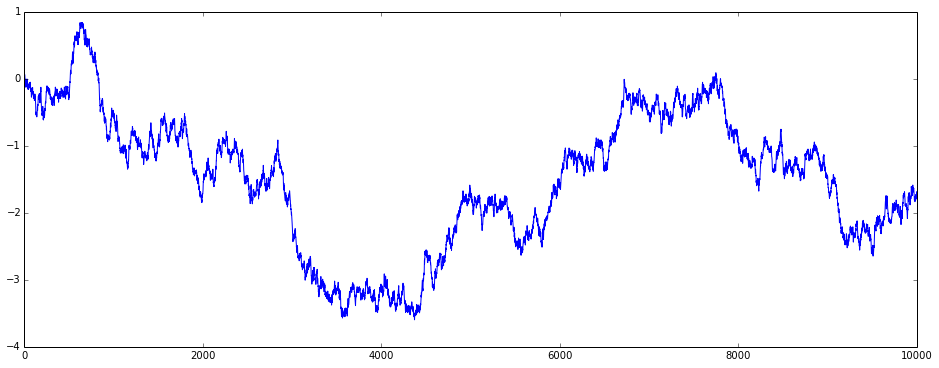
\includegraphics[width=0.9\textwidth]{img/coint-example4}
 \caption{Time series linear combination using the third cointegration vector}
   \label{fig:cointvectors5}
\end{minipage}
\end{figure}


This example shows how cointegration vectors describes the stable relations
between the processes by linear relations that are more stationary than the
original process. Cointegration vectors can be obtained using the Johansen method which gives with a certain probability the number of significant vectors. Figures    
\ref{fig:cointvectors3}, \ref{fig:cointvectors4}  and \ref{fig:cointvectors5}  shows the linear combinations obtained using cointegration vectors given by Johansen method. The method confirm that only two vectors are found and the third one given doesn't result in a I(0) process.

$\blacksquare$

\section{Unit root tests}
Many economic and financial time series exhibit trending behaviour or non-stationary behaviour in the mean or variance. An important econometric task is to determine the type of non-stationary. For trend stationary I(0) time series a time-trend regression is appropriate. For I(1) time series taking first differences transforms it into a stationary one.  For cointegration to determine if time series are I(1) is mandatory to model their long-run relationship. In order to determine if a time series is an a I(1) or I(0) process unit root tests are used. Several tests have been developed but the most widely used is an extension of the Dickey and Fuller test \cite{dickey1979} called the Augmented Dickey-Fuller (ADF) test developed in 1984 by Said and Dickey in 1984\cite{said1984}.

The ADF test tests the null hypothesis that a time series $y_t$ is I(1) against the alternative that it is I(0), assuming that the dynamics in the data have an ARMA structure. The ADF test is based on estimating the test regression:

\begin{equation}
\label{eq:adftest}
y_t = \boldsymbol{\beta}^\top \mathbb{D}_t + \phi y_{t-1} + \sum_{j=1}^p \Psi_j \Delta y_{t-j} + \epsilon_t
\end{equation}

\noindent where $\mathbb{D}_t$ is a vector of deterministic terms. Lag length $p$ has to be determined when applying the test, Akaike Information Criteria (AIC) is commonly used to determine it.
The p-lagged difference terms $\Delta y_{t-j}$ are used to approximate an ARMA process and the value of $p$ is set so that the error $\epsilon_t$ is serially uncorrelated. 
Under the null hypothesis, $y_t$ is I(1) which implies that $\phi=1$. 
The test statistic is the following:

\[
\text{ADF}_t = \frac{\hat{\phi} -1}{SE(\phi)}
\]
\noindent where SE is the standard error.

The $\text{ADF}_t$ statistic is based on the least squares estimates of equation \ref{eq:adftest}.




\section{Volatility in the financial markets}
In financial markets, volatility is one of the key elements to model the
stochastic dynamic behaviour of financial assets. This is mainly because
volatility gives a measure of uncertainty about future returns and it is often
viewed as an indicator of the vulnerability of financial markets. It is also
important as an input parameter in problems like derivative pricing, hedging
and portfolio management.  For example, in option pricing we need to known
first the volatility of the underlying asset before pricing an option. 

Besides, volatility provides important information for studying asset returns
because the latter are largely uncorrelated and nonlinearly dependent. However,
it has been found that volatility exhibits significant autocorrelation and
predictable patterns~\cite{poon+granger2003} and  many models have been
proposed to forecast its behaviour. 

The volatility of the data is due to a large number of factors affecting the
market, with some of them directly measurable such as historical prices,
trends, supply and demand. However, others such as monetary policies and news
are not directly measurable and are included in other models out of the scope
of this thesis. 


Despite the fact variance and volatility are related, they are not the same concept. Variance is a measure of distribution of returns and is not necessarily
bound by any time period.  Volatility is a measure of the standard deviation
(square root of the variance) over a certain time interval. In finance,
variance and volatility both gives you a sense of an asset's risk. Variance
gives you a sense of the risk in the asset over its lifetime, while volatility
gives you a sense of the movement of the asset in, for example, the past month or the
past year. The main underlying difference is in their definition. Variance has a
fixed mathematical definition, however volatility does not as such. Volatility
is said to be the measure of fluctuations of a process.

Volatility is a subjective term, whereas variance is an objective term i.e.
given the data you can definitely find the variance, while you can't find
volatility just having the data. Volatility is associated with the process, and
not with the data. In order to know the volatility you need to have an idea of the process i.e you
need to have an observation of the dispersion of the process. All the different
processes will have different methods to compute volatilities based on the
underlying assumptions of the process.  

\subsection{Types of volatility}

The volatility of a stock is not directly observable~\cite{tsay2005,engle1993}. For example, daily volatility is not directly observable from only daily returns because there is only one observation in a trading day.  If intraday data is available, then volatility could be estimated. However, intraday returns are not the only explanatory variables for volatility and several estimators have been proposed. These estimators are observable variables that are related to the latent variable of interest called volatility proxies~\cite{devilderetal2007}. Examples of volatility proxies are the following: 



\subsubsection{realized volatility} is also known as historic volatility and
it is the actual variance in the price of a stock over time.
Realized volatility is measured in terms of the standard deviation
using the historical stock prices. It is commonly calculated based on
intraday price returns:
\begin{equation}
\label{eq:retintra}
r_{t,n}=100(\ln(p_{t,n}) - \ln(p_{t,n-1}))
\end{equation}
\noindent where $p_{t,n}$ is the price observed at day $t=1,\dots,T$ and
intraday sample $n=2,\dots,N$. Realized volatility is defined as:
\begin{equation}
\label{eq:rv}
    \hat{\sigma}(t) = \sum_{n=1}^N r_{t,n}^2 \, , 
\end{equation}
\noindent where $N$ is the number of intraday samples and $T$ is the
number of days. 
In order to include overnight returns, Hansen and
Lunde~\cite{hansen+lunde2005} introduced a scaling version of
realized volatility using the following definitions:
\begin{eqnarray}
r_{t}&=&100(\ln(p_{t,N}) - \ln(p_{t-1,N})) \label{eq: ret 1} \\
\bar{\rho}(t) &=& \sum_{t=1}^T r_{t}^2  \label{eq: ret 2} \, .
\end{eqnarray}
\noindent where equation~(\ref{eq: ret 1}) represents overnight 
returns and the volatility as 
equation~(\ref{eq: ret 2}), where $p_{t,N}$ is the last intraday 
sample at day $t$. The scaled realized volatility $\rho(t)$ is 
defined as:
\begin{eqnarray}
\label{eq:srv}
\rho(t) = \gamma \hat{\rho}(t) \, , \qquad & \qquad \gamma = \displaystyle \frac{\bar{\rho}(t)}{\displaystyle\sum_{t=1}^T \hat{\rho}(t)}
\end{eqnarray}
Realized volatility has also been defined as the absolute value return or as
the mean of the sum of intraday squared returns at short intervals of time. The
majority of research carried out in the literature obtain the daily volatility
as the daily squared returns as is shown in equation~(\ref{eq: ret 2}).
However, it has been proven that this measurement noise is too high for
observing the true volatility process~\cite{andersen+bollerslev1998}. Hansen
and Lunde~\cite{hansen+lunde2006} stated that the use of a noisy proxy could
result in an inferior model being chosen as the best one. The realized
volatility, as calculated by the cumulative sum of squared intraday returns and
shown in equation (\ref{eq:rv}), is less noisy and doesn't lead to choosing an
inferior model.   
\subsubsection{implied volatility volatility} not only can be extracted from returns
but it can also be derived from option or future pricing models.  The
volatility obtained corresponds to the market's prediction of future
volatility. In finance, an option is a derivative, that is, a contract which
gives the owner the right, but not the obligation to buy or sell an underlying
asset at a given price called strike price. An option can be executed at any
time before an expiration date previously defined no matter what price the
underlying asset has. For example, the Black-Scholes model~\cite{black1973}
determines the fair option value based on stock price, strike price, time to
option expiration, the interest rate and volatility. These are known or can be
easily obtained from the market, excepting by volatility which must be
estimated. However, rather than assuming a volatility a priori and computing
option prices from it, the model can be used to estimate volatility at given
prices, time to expiration and strike price. This obtained volatility is called
the implied volatility of an option. Additionally, some models obtain implied
volatility from futures (other derivative from prices). For instance, the
Barone-Adesi and Whaley futures option model~\cite{baroneetal1987} is also used
to determine future volatilities~\cite{hamidetal2004}. Higher implied
volatility is indicative of greater price fluctuation in either direction.
Implied volatility is found by determining the value which makes theoretical
prices equal to market prices. In this way volatility is ``implied'' by the
current market price of the stock.

In finance, an option is a derivative, that is, a contract which gives the owner
the right, but not the obligation to buy or sell an underlying asset at a given
price called strike price. An option can be executed at any time before an
expiration date previously defined no matter what price the underlying asset
has. 

The Black-Scholes formula~\cite{black1973}, developed in the early 1970's, Myron
Scholes, Robert Merton and Fisher Black,  allows to determine an option value
$V$ based on the underlying asset price $S(t)$ at a time $t$ and the following
constant parameters: 

\begin{description}
\item [$\sigma$:] underlying asset price volatility which measures the standard
deviation of the returns
\item [$\mu$:] underlying asset drift which is a measure of the average rate of
growth of the stock
\item[$E$:] option strike or excersice price
\item[$T$:] option date of expiry
\item[$t$:] current time
\item[$r$:] risk-free interest rate
\end{description}

The Black-Scholes model assume that the underlying price $S$ follows a lognormal random walk:

\begin{equation}\label{eq:stockprice}
dS = \mu S dt + \sigma S dB
\end{equation}

\noindent where $B$ is a Brownian motion. This stochastic differential equation
has two components: a deterministic term given by $\mu S dt$ and a random term
given by $\sigma S dX$.

A brownian motion $B$ (also called a Wiener process) is a stochastic process
characterized by the three following properties:

\begin{description}
\item[Continuity:] $B(t)$ is a continuos function
\item[Normal increments:]  $B(t)-B(s)$ has a normal distribution with mean $0$
and variance $t-s$.
\item[Independence of increments:] for every choice of nonnegative real numbers
$0 \leq s_1 <  t_1 \leq \cdots \leq s_n < t_n < \infty$, the increment random
variables $W_{t_1} - W_{s_1}, \cdots, W_{t_n} - W_{s_n}$ are jointly
independent.
\end{description}

An stochastic differential integral has the form:


\begin{equation}
W(T)=\int_0^T f(t)dB(t) \, .
\end{equation}

\noindent This equations is also expressed in an abbreviate form:

\begin{equation}
dW = f(t) dB \, .
\end{equation}

\noindent Therefore, the integral form of the stock price model shown in
equation (\ref{eq:stockprice}) is:

\begin{equation}
S(T)=\int_0^T \mu S(t) dt + \int_0^T \sigma S(t) dB(t)
\end{equation}


Ito's lemma is used to find the differential of a time dependent function of a
stochastic process. In option pricing we need to find the option price $V(S(t))$
which depends on a stochastic stock price model $S(t)$.  $V(S,t)$ is required to
be  differentiable function of $S$ and once differentiable function of $t$.

These are known or can be easily obtained from the market, excepting by
volatility which must be estimated. However, rather than assuming a volatility
a priori and computing option prices from it, the model can be used to estimate
volatility at given prices, time to expiration and strike price. This obtained
volatility is called the implied volatility of an option. Additionally, some
models obtain implied volatility from futures (other derivative from prices). 


For trading strategies, the interest is centred in forecasting realized
volatility over the life of an option and to take advantage when this
volatility differs from the implied volatility. This is called volatility
arbitrage. For example, a trader will buy an option and hedge the underlying
asset if the implied volatility is under the realized volatility. 


\subsection{Volatility methods}

In the existing literature, there are four main classes of asset
return volatility models: the general autoregressive conditional
heteroskedasticity (GARCH) models, the stochastic volatility (SV)
models, the realized volatility models and the machine learning based
models. A comparison of the first three models can be found
in~\cite{wei2012}. 

For many years the most popular methods for estimating financial
volatility were the autoregressive conditional heteroskedasticity
(ARCH) models~\cite{engle1982} and the general ARCH (GARCH)
models~\cite{bollerslev1986}. For instance, the GARCH(1,1) defines
returns $y_t$ and volatility $\sigma_t$ as:

\begin{eqnarray*}
    y_t &=& \sigma_t \epsilon_t \\
     \sigma_t^2 &=& \alpha_0 + \alpha_1 \epsilon_{t-1}^2 + \beta_1
     \sigma_{t-1}^2
\end{eqnarray*}

\noindent where $\epsilon_t$ is standard Gaussian white noise,
$\alpha_0,\alpha_1,\beta_1 \geq 0$ are required to ensure that the
variance will never be negative and $\alpha_1+\beta_1 <1$ is needed to
guarantee a weakly stationary process~\cite{nelson1990}.

Since the introduction of the GARCH models, several extensions have been
proposed, but none of them seems to beat the GARCH(1,1)
model~\cite{lunde+hansen2005}. Despite its popularity, GARCH models have
several limitations: firstly, a time series model may be non-linear in mean
and/or non-linear in variance, but ARCH and GARCH models are non-linear in
variance, but not in mean. Besides, GARCH models often fail to capture highly
irregular phenomena, like wild market fluctuations.  

SV models explain how volatility varies in a random fashion. These models are
useful because they explain why options with different strikes and expirations
dates have different Black-Scholes implied volatilities, phenomenon known as
the volatility smile. This is useful because the Black-Scholes model assumes
that the volatility of the underlying asset is constant which is not always
true. There are several SV models and the most well-known and popular is the
Heston model~\cite{heston1993}. Additional information about SV models can be
found in~\cite{shephard1995}. 

The realized volatility constructed from high frequency intraday returns gave
rise to the realized volatility models mainly because the realized volatility
series is much more homoskedastic and seems to be a long memory
process~\cite{andersonetal2003}. For realized volatility, the autoregressive
fractionally integrated moving average (ARFIMA) process emerged as a standard
model~\cite{chenetal2010} and many variations have been studied, but all of
them produce similar forecasting results to the ARFIMA(1,d,1)
model~\cite{koopmanetal2005}.  

On the other hand, machine learning based models, especially artificial neural
networks (ANN) and support vector machines (SVM) have arisen as an alternative
to forecast volatility. ANN is a statistical technique inspired by biological
neural networks which is capable of changing its structure based on external or
internal information during a training phase~\cite{sammut2011}. SVM are
supervised learning models for classification analysis which recognize patterns
finding a separating hyperplane. An extension for regression analysis is known
as support vector regression (SVR). 

Since machine learning models and in particular ANN do not require assumptions
about the data (gaussianity for example) and allow more explanatory variables
than returns to be included, they have become widely used in solving financial
problems, specially volatility
forecasting~\cite{hamidetal2004,donaldsonetal1997}. There are also many works
focused on the using of SVM in volatility
forecasting~\cite{shiyietal2008,shiyietal2010,gavrishchaka2006,vasilios2012}. 

However, just as with ANN, SVMs have scalability problems because their
training process is computationally intensive and it is done in batch mode. The
scalability problem worsens when new additional training data is available and
a re-training process from scratch needs to be done. This problem can be
avoided using online machine learning algorithms that allow one instance at a
time to be processed with low computationally expensive calculations.



%\section{Vector Autoregressive Models}\label{sec:varvec}
\section{Multivariate Time Series modelling}

The vector autoregressive VAR($p$) model \cite{sims1980} is one of the most easy to use, successful and flexible models for the analysis of multivariate time series. It is a natural extension of the univariate autoregressive (AR) model. The VAR model has proven to be useful for describing the dynamic behaviour of economic and financial time series.
VAR is a general framework describing the behaviour of a
set of $l$ endogenous variables as a linear combination of their last $p$
values, where $l,p\in\mathbb{N}$. 
In our case, each one of these $l$ variables is a scalar time series
$y_{\lambda,t}$, $\lambda=1,\dots,l$, and we represent them all together
at time $t$ by the the vector time series:
\begin{equation}
\label{eq:variables}
\mathbf{y}_t = 
\begin{bmatrix} y_{1,t} & y_{2,t} & \dots & y_{l,t} \end{bmatrix}^\top.
\end{equation}
\noindent
Notice that the vectors $\mathbf{y}_t$ are assumed to be $l$-dimensional.

The VAR($p$) model describes the behaviour of a dependent variable in terms of
its own lagged values and the lags of the others variables in the system. The
model with $p$ lags is formulated as the system of $N$:
\begin{align}
\label{eq:var}
\mathbf{y}_t 
= \boldsymbol{\Phi}_1 \mathbf{y}_{t-1} +
  \boldsymbol{\Phi}_2 \mathbf{y}_{t-2} + \dots +
  \boldsymbol{\Phi}_p\mathbf{y}_{t-p} +
  \mathbf{c} + \boldsymbol{\epsilon}_t \nonumber \\
t=p+1,\dots,N,
\end{align}
\noindent where 
$\boldsymbol{\Phi}_1, \boldsymbol{\Phi}_2,\dots,\boldsymbol{\Phi}_p$
are $l\times l$-matrices of real coefficients,
$\boldsymbol{\epsilon}_{p+1},
 \boldsymbol{\epsilon}_{p+2}, \dots, \boldsymbol{\epsilon}_N$ 
are error terms, $\mathbf{c}$ is a constant vector and $N$ is the total
number of samples.

Notice that, regarding our notation of section (\ref{sec:coint}),
we have here 
$\mathbf{y}_t^0 = \mathbf{y}_t$,
$\mathbf{y}_t^\nu = \mathbf{y}_{t-\nu}$ and
the $\lambda$-th component of the vector time series $\mathbf{y}_t^\nu$
is the scalar time series $y_{\lambda,t}^\nu$, where $\nu=1,\dots,p$ and
$\lambda=1,\dots,l$.
Transposing each equation of the system (\ref{eq:var}) we can write
the VAR($p$) model in block-matrix form as:
\begin{equation}\label{eq:vareq}
\mathbf{Y} = \mathbf{A} \mathbf{X} + \mathbf{E} \, , 
\end{equation}
%%
\noindent where:
%%
\begin{alignat}{2}
\mathbf{Y}
&= \begin{bmatrix}
   \mathbf{y}_{p+1}^\top \\
   \mathbf{y}_{p+2}^\top \\
   \vdots \\
   \mathbf{y}_N^\top
   \end{bmatrix}_{(N-p)\times l}
&\quad
\mathbf{A}
&= \begin{pmat}[{...|}]
   \mathbf{y}_p^\top & \mathbf{y}_{p-1}^\top & \dots 
                    & \mathbf{y}_1^\top & 1 \cr
   \mathbf{y}_{p+1}^\top & \mathbf{y}_p^\top & \dots
                       & \mathbf{y}_2^\top & 1 \cr
   \vdots & \vdots & \ddots & \vdots & \vdots \cr
   \mathbf{y}_{N-1}^\top & \mathbf{y}_{N-2}^\top & \dots 
                       & \mathbf{y}_{N-p}^\top & 1 \cr
   \end{pmat}_{(N-p)\times(pl+1)} \\
\mathbf{X}
&= \begin{bmatrix}
   \boldsymbol{\Phi}_1^\top \\
   \boldsymbol{\Phi}_2^\top \\
   \vdots \\
   \boldsymbol{\Phi}_p^\top \\
   \mathbf{c}^\top
   \end{bmatrix}_{(pl+1)\times l}
&\quad
\mathbf{E}
&= \begin{bmatrix}
   \boldsymbol{\epsilon}_{p+1}^\top \\
   \boldsymbol{\epsilon}_{p+2}^\top \\
   \vdots \\
   \boldsymbol{\epsilon}_N^\top \\
   \end{bmatrix}_{(N-p)\times l}
\end{alignat}
Taking into account the error term $\mathbf{E}$, equation~(\ref{eq:vareq}) 
can be solved with respect to $\mathbf{X}$ using the ordinary least
squares estimation.

\section{Vector error correction model}
Vector error correction model (VECM)  \cite{engle87} is a special form of a VAR model for I(1) variables that are also
cointegrated~\cite{banerjee1993}.

It is obtained re-writing equation (\ref{eq:var}) in terms of the new
variable $\Delta\mathbf{y}_t=\mathbf{y}_t-\mathbf{y}_{t-1}$.
The VECM model, expressed in terms those differences, takes the form:
\begin{equation}\label{eq:vec}
\Delta \mathbf{y}_t 
= \boldsymbol{\Omega}\,\mathbf{y}_{t-1}
  + \sum_{i=1}^{p-1} \boldsymbol{\Phi}_i^*\,\Delta\mathbf{y}_{t-i}
  + \mathbf{c} + \boldsymbol{\epsilon}_t\,,
\end{equation}
\noindent
where the coefficients matrices $\boldsymbol{\Phi}_i^*$ and 
$\boldsymbol{\Omega}$, expressed in terms of the matrices
$\boldsymbol{\Phi}_i$ of (\ref{eq:var}), are:
\begin{align*}
\boldsymbol{\Phi}_i^* 
&:= -\sum_{j=i+1}^{p}\boldsymbol{\Phi}_j\,, \\
\boldsymbol{\Omega}
&:= -\left( \mathbb{I} - \boldsymbol{\Phi}_1 - \dots 
    - \boldsymbol{\phi}_p \right)\,. 
\end{align*}
The following well known properties of the matrix $\boldsymbol{\Omega}$
\cite{johansen1995} will be useful in the sequel:
\begin{itemize}
\item
If $\boldsymbol{\Omega} = \mathbf{0}$, there is no cointegration.
\item 
If $rank(\boldsymbol{\Omega})=l$, i.e., if $\boldsymbol{\Omega}$ has
full rank, then the time series are not I(1) but stationary.
\item
If $rank(\boldsymbol{\Omega})=r$, $0<r<l$, then there is cointegration
and the matrix $\boldsymbol{\Omega}$ can be expressed as
$\boldsymbol{\Omega}=\boldsymbol{\alpha\beta}^\top$, where $\boldsymbol{\alpha}$
and $\boldsymbol{\beta}$ are
$l\times r$ matrices and
$\text{rank}(\boldsymbol{\alpha})=\text{rank}(\boldsymbol{\beta})=r$.
\item
The columns of $\boldsymbol{\beta}$ contains the cointegration vectors and the rows of
$\boldsymbol{\alpha}$ correspond with the adjusted vectors. 
$\boldsymbol{\beta}$ is obtained by Johansen procedure~\cite{johansen1988},
whereas $\boldsymbol{\alpha}$ has to be determined as a variable in the VECM.
\end{itemize}
It is worth noticing that the factorization of the matrix
$\boldsymbol\Omega$ is not unique, since for any $r \times r$
nonsingular matrix $\mathbf{H}$, $\boldsymbol{\alpha}^*:=\boldsymbol{\alpha}\mathbf{H}$,
and $\boldsymbol{\beta}^*=\boldsymbol{\beta}(\mathbf{H}^{-1})^\top$ we have
$\boldsymbol{\alpha\beta}^\top=\boldsymbol{\alpha}^*(\boldsymbol{\beta}^*)^\top$.
If cointegration exists, then equation (\ref{eq:vec}) can be written
as follows:
\begin{equation}\label{eq:vecfull}
\Delta\mathbf{y}_t 
= \boldsymbol{\alpha\beta}^\top\mathbf{y}_{t-1} 
  + \sum_{i=1}^{p-1}\boldsymbol{\Phi}_i^*\,\Delta\mathbf{y}_{t-i}
  + \mathbf{c} + \boldsymbol{\epsilon}_t\,,
\end{equation}
\noindent
which is a VAR model but for time series differences.


Transposing each equation of the system (\ref{eq:vecfull}) we can write
the VECM($p$) model in block-matrix form as:
\begin{equation}\label{eq:vareq}
\mathbf{Y} = 
\mathbf{A} \mathbf{X} + 
\mathbf{E} \, , 
\end{equation}

\noindent where $\mathbf{Y}$ dimension is $((N-p)\times l)$, $\mathbf{A}$
dimension is $((N-p)\times(r+(p-1)l +1))$, $\mathbf{X}$ dimension is $((r+(p-1)l
+1)\times l)$ and $\mathbf{E}$ dimension is $((N-p)\times l)$:

\begin{align}
\label{eq:vecY}
\mathbf{Y}
= \begin{bmatrix}
   \Delta\mathbf{y}_{p+1}^\top \\
   \Delta\mathbf{y}_{p+2}^\top \\
   \vdots \\
   \Delta\mathbf{y}_N^\top
   \end{bmatrix}
\end{align}

\begin{align}
\label{eq:vecX}
\mathbf{X}
= \begin{bmatrix}
   \boldsymbol{\alpha}^\top \\
   \boldsymbol{\Phi}_1^{*\top} \\
   \boldsymbol{\Phi}_2^{*\top} \\
   \vdots \\
   \boldsymbol{\Phi}_{p-1}^{*\top} \\
   \mathbf{c}^\top
   \end{bmatrix}
\end{align}

\begin{align}
\label{eq:vecX}
\mathbf{E}
= \begin{bmatrix}
   \boldsymbol{\epsilon}_{p+1}^\top \\
   \boldsymbol{\epsilon}_{p+2}^\top \\
   \vdots \\
   \boldsymbol{\epsilon}_N^\top \\
   \end{bmatrix}
\end{align}

\noindent and 

\begin{align}
\label{eq:vecA}
\mathbf{A}
&= \begin{pmat}[{....|}]
   \mathbf{y}_p^\top \boldsymbol{\beta} & \Delta \mathbf{y}_p^\top & \Delta\mathbf{y}_{p-1}^\top & \dots 
                    & \Delta\mathbf{y}_2^\top & 1 \cr
   \mathbf{y}_{p+1}^\top  \boldsymbol{\beta} &\Delta\mathbf{y}_{p+1}^\top & \Delta\mathbf{y}_p^\top & \dots
                       & \Delta\mathbf{y}_3^\top & 1 \cr
   \vdots & \vdots & \vdots & \ddots & \vdots & \vdots \cr
   \mathbf{y}_{N-1}^\top  \boldsymbol{\beta} &\Delta\mathbf{y}_{N-1}^\top & \Delta\mathbf{y}_{N-2}^\top & \dots 
                       & \Delta\mathbf{y}_{N-p-1}^\top & 1 \cr
   \end{pmat}\, .
\end{align}



Taking into account the error term $\mathbf{E}$, equation~(\ref{eq:vareq}) 
can be solved with respect to $\mathbf{X}$ using the ordinary least
squares estimation (see section \ref{sec:OLS}).

Conventional regression estimators, including VARs, have good properties when applied to covariance-stationary time series, but encounter difficulties when applied to non stationary or integrated processes.

These difficulties were illustrated by Granger and Newbold in 1974 \cite{granger1974} when they introduced the concept of spurious regressions (see section \ref{sec:spurious}). In 1982, Nelson and Plosser  \cite{nelson1982} showed that unit roots might be present in a wide variety of macroeconomic series
in levels or logarithms. This finding gave rise to the industry of unit root testing, and
the implication that variables should be rendered stationary by
differencing before they are included in an econometric model.
Further theoretical developments by Granger and Engle in 1987 \cite{engle87} raised the possibility that two or more integrated, non stationary time series might be cointegrated, so that some linear combination of these series could be stationary even though each series were not. 

If two series are both integrated (of order one, or I(1)) we could model
their interrelationship by taking first differences of each series and
including the differences in a VAR or a structural model.
However, this approach would be suboptimal if it was determined that
these series are indeed cointegrated. In that case, the VAR only
express the short-run responses of these series to innovations in each
series. This implies that the simple regression in first differences is
misspecified.
If the series are cointegrated, they move together in the long-run. A
VAR in first differences will not capture those long-run tendencies.
VECM fit to the first differences of the non stationary variables, but a lagged error-correction term is added to the relationship representing the long-run relationship.

In finance, many economic time series are revealed to be stationary when they
are differentiated and moreover cointegration restrictions often improve
forecasting \cite{duy1998}. Therefore, VECM has been widely adopted in
finance: \cite{mukherjee1995}, \cite{maysami2000}, \cite{arestis2001} and
\cite{seong2013} to name a few. Pair
trading is a very common example of a cointegration
application \cite{herlemont2003} but also can also be extended to a larger set
of variables \cite{mukherjee1995}, \cite{engle2004}.



\chapter{Machine Learning Models}
Machine learning is a scientific discipline focused on the development of algorithms focused on learning from examples. This idea has become central to the design of search engines, robots systems and forecasts applications which process large data sets. However, machines require an extended training period when developing algorithms to predict future behaviour such as financial time series forecasting where new data is available in a short period of time.  Online machine learning techniques tackle this problem and allow to update the model with new data or to compute a new model using less data allowing to give a response in a short period of time.

\vspace{0.5cm} 

\section{Introduction}
Machine Learning (ML) studies computer algorithms for learning
something such as to complete a task, to make accurate predictions or to behave intelligently. The learning is always based on samples and the objective is about to do better in the future based on the past experiences in an automatic way. ML is a subarea of artificial intelligence and broadly intersects with other fields such as statistics, mathematics, physics and computer science. 
There are many examples of machine learning problems: time series forecasting, image processing, face detection, spam filtering, weather prediction, search engines, among many others.

ML models are often more accurate than what can be created through direct programming. The reason is that ML models are data driven and are able to examine large amounts of data.

There are three types of ML classified depending on the nature of the learning input or output available to a learning system.
\begin{description}
\item[supervised learning]  the input data is a tuple which contains the example input and its desired outputs (also called labels). The list of tuples is called the training set. The concept of supervised learning comes from the supervisor, acting as a teacher in the learning process. The goal is to learn a general rule that maps inputs to outputs optimising a target function. There are two related problem types in supervised learning: classification and regression problems \cite{bishop2006}. Its two mainstream approaches are: support vector machines (SVMs) \cite{vapnik1998} and ensemble learning \cite{breiman1998}. Furthermore supervised learning can be categorised into offline or batch learning and online learning (see section \ref{sec:onoffline}). 
\item[unsupervised learning] also known as clustering \cite{ben2005}. In this type of learning no labels are given and the system has to find a structure on its own, discovering hidden patterns in data.
\item[reinforcement learning] is the problem faced by an agent that must learn 
through trial-and-error interactions with a dynamic environment. It is based on programming agents by reward and punishment without needing to specify how the task is to be achieved \cite{sutton1998}.
\end{description}



%%% Learning problem. Ac;a ma;ana, formulas y descripcion de tallada del problema de aprendizaje


\section{Statistical learning theory} \label{sec:mltheory}

All ML problems can be viewed as optimisation problems. The ML core task is to define a learning criterion, i.e the function to be optimised. 

In this thesis we will emphasised the supervised learning problem since it is the most common way of modelling financial problems.

Supervised learning consists in to find a learning function $f: X \rightarrow Y$ which models a set of examples called training set $S$ which have been drawn randomly and independently according to a unknown joint distribution function $p(x,y)$ on $X \times Y$:


$$
S= \{(x_1,y_1),\,(x_2,y_2),\dots\,,\,(x_n,y_n)\} \in \mathcal{S}, (x_i,y_i) \in X\times Y \quad \forall i = 1\dots n
$$

\noindent where $X \subseteq \mathbb{R}^m$ and $Y = \mathbb{R}$ in case of regression problems and $Y = \{1,-1\}$  if it is a classification problem. 

A learning algorithm $\mathcal{A}$ takes as input a data set $S \in \mathcal{S}$ and output a function $f_S$:

\begin{eqnarray*}
\mathcal{A}: \mathcal{S} &\rightarrow & \mathcal{H} \\
S &\rightarrow &\mathcal{A}(S) = f_S
\end{eqnarray*}

\noindent where $\mathcal{H}$ is called the hypothesis space, is the space of functions that the algorithm is allowed to search. The selection of $f_S$ is based on a loss function $V(f(x),y)$ which expected risk has to be minimised.

\[
E[V(f(x),y)] = \int V(f(x),y) dp(x,y)
\]

\noindent $V(f(x),y)$ denote the price paid for mistakes. Therefore, $V(f(x),y)=0$ if$f(x)=y$.

For regression, the most common loss function is square loss or L2 loss function:
\begin{equation}
\label{eq:l2loss}
V(f(x),y) = (f(x)-y)^2
\end{equation}
\noindent another option is the L1 loss
\begin{equation}
\label{eq:l1loss}
V(f(x),y) = |f(x)-y| \, .
\end{equation}
\noindent the choice of loss function here gives rise to several well-known learning algorithms such as regularised least squares and support vector machines. %verificar esto7776

Since the true distribution is unknown and only training samples are available, the objective is to estimate a function $\hat{f}$ through empirical risk (training error) minimisation (ERM): 

\begin{equation} 
\label{eq:erm}
R_{\text{emp}}[f] = \frac{1}{n} \sum_{i=1}^n V(f(x),y)
\end{equation}

\subsection{Learning algorithms}
In all learning algorithms that are trained from example data, there is a tradeoff \cite{dietterich2003} between three factors:
\begin{description}
\item[Complexity of the hypothesis class] for best generalisation, we should adjust the complexity of the learner model $\hat{f}$ to the complexity of the data $f$. In polynomial regression, the complexity parameter is the order of the fitted polynomial, and therefore we need to find a way to choose the best order that minimises the generalisation error, that is, tune the complexity of the model to best fit the complexity of the function inherent in the data.
\item[Generalisation accuracy on new examples] is the capability of the algorithm to generate the right output for an input instance outside the training set.
\item[The amount of training data]  generally generalisation accuracy increases as the amount of training data increases.
\end{description}

Very complex models will fit the training data better (low bias) but it could overfit it and generalise poorly (high variance), this is also called the bias-variance tradeoff.  Generalisation accuracy can sometimes be improved with more training data. The figure \ref{fig:tradeoff} illustrates how generalisation accuracy depends on the complexity of the model and the amount of training data.

\begin{figure}[!h]
  \centering
  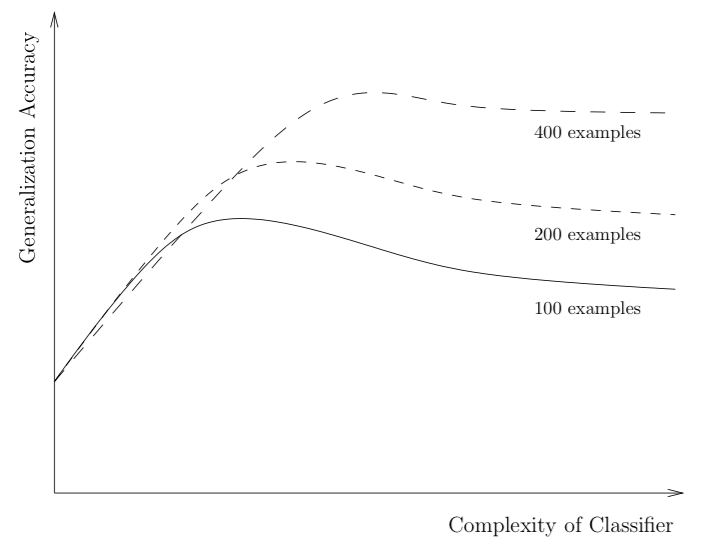
\includegraphics[width=0.8\textwidth]{img/3tradeoff}
  \caption{Triple tradeoff in empirical learning}
  \label{fig:tradeoff}
\end{figure}

\subsection{The bias-variance tradeoff}

Models learning error can be split into two main components: error due to bias and error due to variance. Bias measures how far off in general these models' predictions are from the correct value. Variance is taken as the variability of a model prediction for a given data point.

If we have a learning model $\hat{f}$, its expected generalisation error on an unseen or testing sample $x$ can be decomposed as follows:

\begin{align}
\mathrm{E}\Big[\big(y - \hat{f}(x)\big)^2\Big]
 & = \mathrm{Bias}\big[\hat{f}(x)\big]^2 + \mathrm{Var}\big[\hat{f}(x)\big] + \sigma^2
\end{align}
\noindent where:
\begin{align*}
 \mathrm{Bias}\big[\hat{f}(x)\big] &= \mathrm{E}\big[\hat{f}(x)\big] - f(x) \\
 \mathrm{Var}\big[\hat{f}(x)\big] &= \mathrm{E}\Big[ \big( \hat{f}(x) - \mathrm{E}[\hat{f}(x)] \big)^2 \Big] 
\end{align*}


Bias is introduced by the model selection. Therefore the model building process is repeated (through resampling) and substantially different averages of prediction values are obtained, bias will be high. The error due to variance is the amount by which the prediction, over one training set, differs from the expected predicted value, over all the training sets. Variance measures how inconsistent are the predictions from one another, over different training sets, not whether they are accurate or not.

This generalisation error is unknown, but it can be estimated using a training sample, a testing sample or by estimating the model complexity. Figure \ref{fig:traintesterror} shows prediction error for training and testing sample.  In general, in the training sample prediction error is decreasing with more complex models but it overfit the data and it is not a good model for the test data. Figure \ref{fig:bvtradeoff} shows how testing error can be decomposed into bias and variance components. The best model will be the one has a balance between bias and variance.

\begin{figure}[!h]
  \centering
  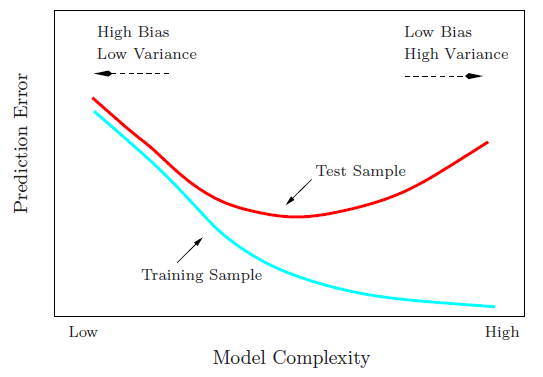
\includegraphics[width=0.8\textwidth]{img/model_complexity}
  \caption{Training and test error}
  \label{fig:traintesterror}
\end{figure}


The objective is to simultaneously reduce bias and variance as much as possible in order to obtain as accurate model as is feasible.  However, there is a tradeoff to be made when selecting models. Models that exhibit small variance and high bias underfit the truth target.  Models that exhibit high variance and low bias overfit the truth target.

This bias-variance tradeoff is the reason why in order to obtain the best model, data is usually broken in three subsets: training set, validation set and testing set. Training set is used to determine the model, validation set is used to estimate the generalisation error and finally testing set is used to estimate the accuracy of the model. Usually the partition is 50\% for training set, 25\% for validation and 25\% for testing purposes. This procedure can be extended to a Cross Validation (CV) procedure \cite{geisser1975}, usually used when the amount of data is limited. Various splitting strategies lead to various CV estimates. In K-fold cross-validation the training data is divided randomly into K distinct subsets, then the network is trained using K-1 subsets, and tested on the remaining subset. The process of training and testing is then repeated for each of the K possible choices of the subset omitted from the training. The average performance on the K omitted subsets is then our estimate of the generalisation performance.

\begin{figure}[!h]
  \centering
  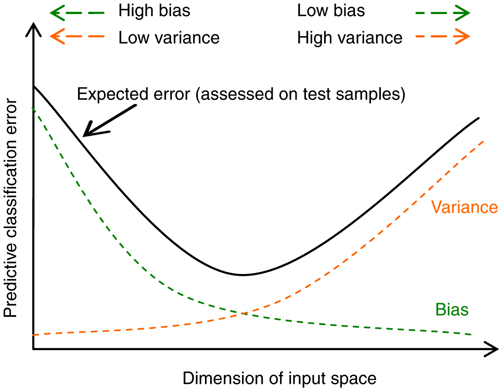
\includegraphics[width=0.8\textwidth]{img/biasvariancetradeoff}
  \caption{Bias variance tradeoff}
  \label{fig:bvtradeoff}
\end{figure}

Another way to control the complexity of the model is to include in the optimisation function not only the generalisation error but a penalisation of high complex models. 


\subsection{Regularization}
Since ERM is an ill-posed problem, Tikhonov introduced a regularisation which ensures well-posedness and generalisation of ERM, i.e prevents overfit, by constraining the hypothesis space $\mathcal{H}$ usually called regularised ERM or Tikhonov regularisation.

Tikhonov regularisation minimised over the hypothesis space $\mathcal{H}$ for a fixed positive parameter $\lambda$ the following:

\begin{equation} 
\label{eq:rerm}
R_{\text{emp}}[f] = \frac{1}{n} \sum_{i=1}^n V(f(x),y) + \lambda \mathcal{R}(f)
\end{equation}

\noindent where $\mathcal{R}(f)$ is the regulariser, a penalisation on $f$.

\subsection{Ridge Regression}
One example of regularisation in linear models is Ridge Regression (RR), which is a regularised least squares method.
The least squares (LS) method is a well known way to solve a regression
problem. 
LS method consists of minimising the sum of squared errors:

\begin{eqnarray*}
\label{eq:lsm}
 J(\mathbf{\phi}) =& \sum_{t=1}^N (f(\mathbf{x}_t)-y_t)^2 \\
 =& \sum_{t=1}^N (\mathbf{\phi}^\top {\mathbf{x}}_t-y_t)^2 \\
 =& \| \mathbf{X}\mathbf{\phi} - \mathbf{Y} \|_2^2 
\end{eqnarray*}

The optimal solution for $\mathbf{\phi}$ is:
\begin{equation*}
\mathbf{\phi}=(\mathbf{X}^\top
\mathbf{X})^{-1}\mathbf{X}^\top \mathbf{Y}
\end{equation*}

In order to avoid the singularity of the matrix $\mathbf{X}^\top \mathbf{X}$, a regularisation term is introduced: 

\begin{equation*}
\label{eq:problem} 
J(\mathbf{\phi}) =  \| \mathbf{X}\mathbf{\phi} - \mathbf{Y} \|_2^2  + \lambda
 \| \mathbf{\phi}\| ^2
\end{equation*}

\noindent which optimal solution $\mathbf{\phi}_*$ is well known: 

\begin{equation*}
\label{eq:optsolRR}
\mathbf{\phi}_*=(\mathbf{X}^\top \mathbf{X}+\lambda \mathbb{I})^{-1}\mathbf{X}^\top y \, ,
\end{equation*}

\texttt{Demo}
\begin{eqnarray*}
J(\mathbf{\phi}) &=&  \| \mathbf{X}\mathbf{\phi} - \mathbf{Y} \|_2^2  + \lambda
 \| \mathbf{\phi}\| ^2 \\
 &=&  \sum_{t=1}^N (\mathbf{\phi}^\top {\bf x}_t-y_t)^2 + \lambda \sum_{i=1}^p \phi_i^2 \\
 &=& (\phi^\top x_1-y_1)^2 + \dots + (\phi^\top x_N-y_N)^2 + \lambda (\phi_1^2+\dots+\phi_p^2)
\end{eqnarray*}
\noindent taking derivatives
 \begin{eqnarray*}
 \frac{\partial J(\mathbf{\phi})}{\partial \phi_1}&=& 
 2(\phi^\top \mathbf{x}_1-y_1)\mathbf{x}_{11} + \dots + 2(\phi^\top \mathbf{x}_N-y_N)\mathbf{x}_{N1} + 2\lambda \phi_1 \\
 &=& 2\mathbf{x}_1^\top(\mathbf{X}\phi-\mathbf{Y}) + 2\lambda\phi_1\\
& \vdots &\\
  \frac{\partial J(\mathbf{\phi})}{\partial \phi_p}&=& 
 2\mathbf{x}_p^\top(\mathbf{X}\phi-\mathbf{Y}) + 2\lambda\phi_p 
\end{eqnarray*}

Then we have that:
\begin{eqnarray*}
\frac{\partial J(\mathbf{\phi})}{\partial \phi}&=& 
 2\mathbf{X}^\top(\mathbf{X}\phi-\mathbf{Y}) + 2\lambda\phi
\end{eqnarray*}
Since $\frac{\partial J(\mathbf{\phi})}{\partial \phi}=0$ we have:
\begin{eqnarray*}
2\mathbf{X}^\top(\mathbf{X}\phi-\mathbf{Y}) + 2\lambda\phi&=&0 \\
\mathbf{X}^\top\mathbf{X}\phi - \mathbf{X}^\top\mathbf{Y} + \lambda\phi &=& 0\\
(\mathbf{X}^\top\mathbf{X}+\lambda\mathbb{I})\phi &=&  \mathbf{X}^\top\mathbf{Y} \\
\phi &=& (\mathbf{X}^\top\mathbf{X}+\lambda\mathbb{I})^{-1}  \mathbf{X}^\top\mathbf{Y}
\end{eqnarray*}


When $\mathbf{X}$ is orthonormal then $\mathbf{X}^\top \mathbf{X} =\mathbb{I}$ and there is a simple relation between the ridge estimator and the OLS estimator:
\begin{eqnarray*}
\phi_* (\lambda) &=& (\mathbf{X}^\top \mathbf{X}+\lambda \mathbb{I})^{-1}\mathbf{X}^\top \mathbf{Y} \\
 &=& (\mathbb{I} + \lambda \mathbb{I})^{-1} \mathbf{X}^\top \mathbf{Y} \\
 &=&(1+\lambda)^{-1} \mathbb{I} \mathbf{X}^\top \mathbf{Y} \\
 &=&(1+\lambda)^{-1} (\mathbf{X}^\top \mathbf{X})^{-1}\mathbf{X}^\top \mathbf{Y} \\
 &=&(1+\lambda)^{-1} \phi
\end{eqnarray*}

\subsection{Machine learning algorithms}
In recent years many successful machine learning applications have been developed. Artificial neural network (ANN) and Support Vector Machines (SVM) have been some of the most popularly used machine learning algorithm. Historically, SVMs emerged after ANN.

ANN is inspired by biological learning systems even though it does not mimic it fully. ANN are organised into layers and have unidirectional connections between the layers, feed-forward network is the most used. 

\begin{figure}[!h]
  \centering
  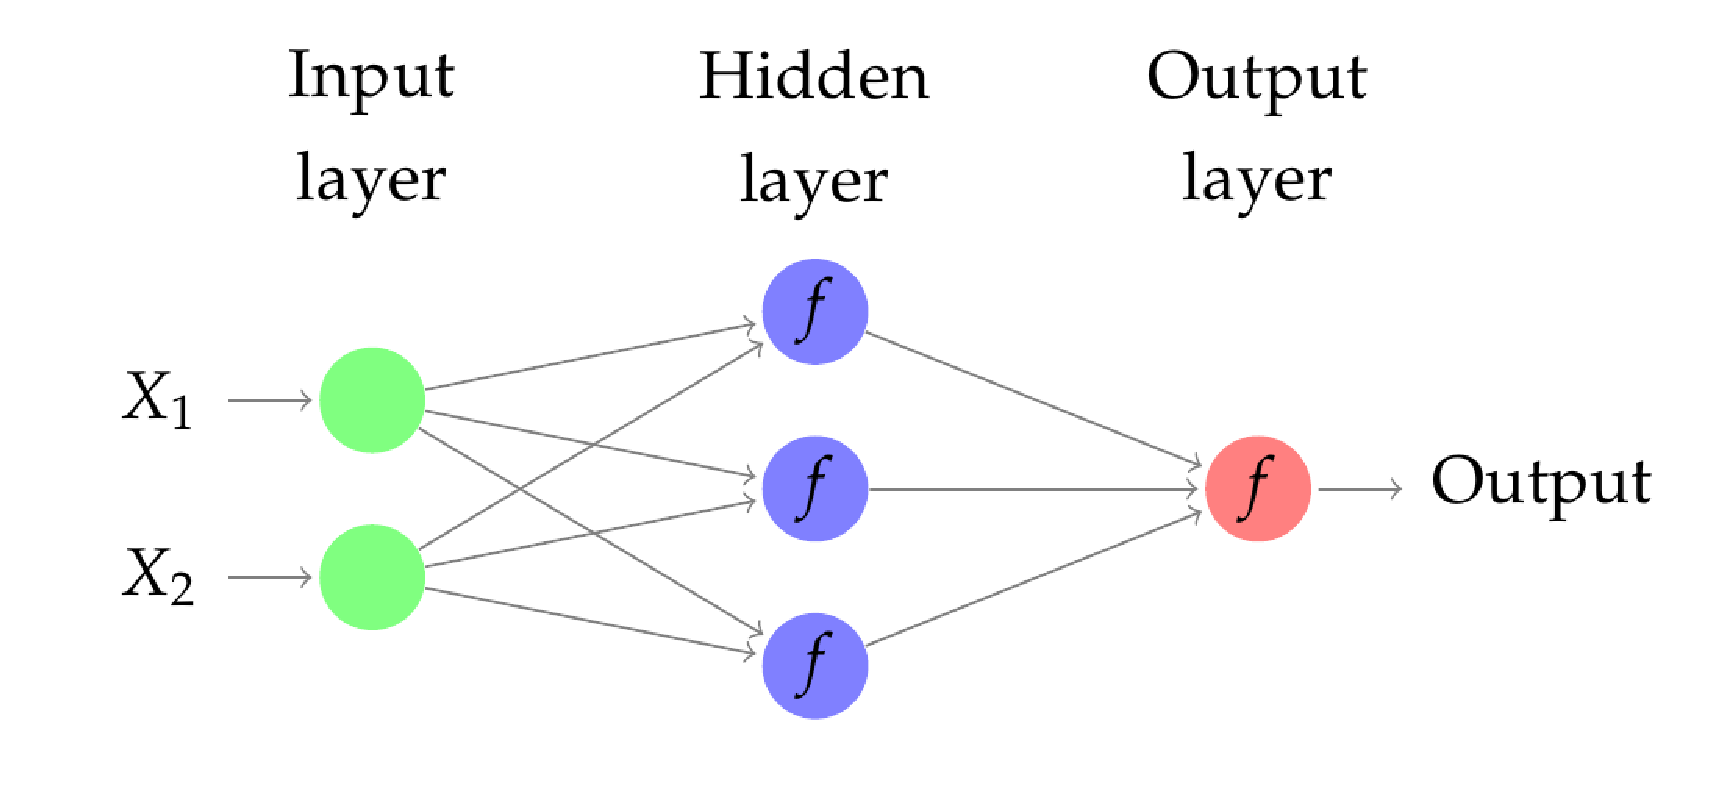
\includegraphics[width=0.8\textwidth]{img/ffn}
  \caption{Feed-forward neural network}
  \label{fig:ffn}
\end{figure}

SVM on the other hand is a relatively new learning algorithm. It can be
similarly used to learn target functions. However, unlike ANN, it is very well founded
based on theory in statistical learning [2]. The major difference between SVM and ANN
is in the error optimization. In ANN, the aim of learning is to obtain a set of weight
values which minimize the training error while in SVM the training error is set to
minimum while training adjust the capacity of the machine. During training, SVM
learned the parameters a?s and the number of support vectors which is equivalent to the
number of hidden units in ANN.
the nodes are artificial
neurons and directed edges are connections between neuron outputs and neuron inputs.
The main characteristics of neural networks are that they have the ability to learn
complex nonlinear input-output relationships, they use sequential training procedures and
they adapt themselves to the data.




Support Vector Machine (SVM) was introduced in 1992 by Vapnik and his coworkers
[3]. In its original form, SVM is a training algorithm for linear classification.
Only later it was used for regression, principal component analysis, novelty detection and
also for non-linear case. SVM tunes the capacity of the classification function by
maximizing the margin between the training patterns and the decision boundary. The
solution is expressed as a linear combination of supporting patterns, which are the subset
of training patterns close to the decision boundary, called the support vectors. 

For nonlinear
case, SVM mapped the data sets of input space into a higher dimensional feature
space, which is linear and the large-margin learning algorithm is then applied. However,
the mapping can be implicitly done by kernel functions. In the high dimensional feature
space, simpler and linear hyper plane classifiers that have maximal margin between the
classes can be obtained.


\subsection{Kernel methods}

Kernel functions may be used to introduce a nonlinear separation
in input space despite the linear classifier in decision space

\section{Online learning} \label{sec:onoffline}

Online learning is a supervised machine learning framework that is useful when we have sequential access to a sample only once.  This differs from the classical batch learning, where there is an entire data set available and the learner can build the internal model without any limits in accessing the data. In batch learning, there is time enough to carefully analyse the dataset, build large predictive models and combine them in a sophisticated way. 

In only learning the goal is the same as batch learning, predicting targets as accurate as possible. For example, stock market prediction can be seen as online learning. The algorithm makes a prediction of the stock, little time after the real stock price is available, this information can be incorporated to the learner to further improve the prediction accuracy. In general, there is too much data available in an online learning setup, the data set grows continuously. Offline learning has equal or superior accuracy compared to online learning when the same amount of data is used.

Classic statistical theory of sequential prediction enforces strong assumptions on the statistical properties of the input sequence (for example, stationary stochastic process). However, these assumptions can be unknown or change over time. In online learning there is no previous assumption about the data and the sequence is allowed to be deterministic, stochastic or even adaptive.  

Moreover, in case we receive data streams, ANN or SVM cannot introduce new information into the model without a re-training process, so we will have to use the same non-updated model until we decide to compute another one if it is possible.  Online learning algorithms allow one example at a time to be introduced into an existing model incrementally~\cite{vovk2005}. This is extremely important when the problem has large data streams and real-time forecasting must be done.  This is the most common scenario when we want to forecast a wide range of data such as stock prices and volatilities, electricity power, intrusion detection, web-mining, server load, etc.  Besides, many problems of high interest in machine learning can be treated as online ones and they can also use these types of algorithms.

The online learning framework was first introduced in the perceptron algorithm~\cite{rosenblatt58}. There are several other widely used online methods such as passive-aggressive~\cite{crammerETall2006}, stochastic gradient descent~\cite{zhang2004}, aggregating algorithm~\cite{vovk2001} and the second order perceptron~\cite{cesa-bianchi2005}.  In~\cite{cesa-bianchi2006} an in-depth analysis of online learning is provided.

The motivation for online learning is to obtain computational efficiency and tackle the shifting problem, i.e. that the distribution of the data is unknown or changes over time. Online learning algorithms can deal with this problem because they have a tracking ability which is a strategy based on retaining weak dependence on past examples by using two types of models: 

\textit{a)} \textbf{memory boundedness:} consists of limiting the number of support vectors in order to improve computational efficiency. One example of this is the budget perceptron~\cite{crammeretal2004} which reduces the number of examples used for prediction. Alternatively, in the forgetron algorithm~\cite{dekeletal2008} the damage caused by removing old examples is discussed, which can be avoided by removing samples with small influences. Other examples are the sliding window kernel (RLS)~\cite{vanvaerenberghetal2006}, which only considers a sliding window of the most recent data, and in \cite{arce+salinas2012} is shown a variant of aggregating algorithm for regression~\cite{vovk2001} considering only a sliding window of the most recent data, optimising also common matrix operations.

\textit{b)} \textbf{weight decay:} one example of this is the shifting perceptron algorithm which implements an exponential decaying scheme for the examples~\cite{cavallantietal2007}.
Performance of an online learning algorithm is measured by the cumulative loss it suffers along its run on a sequence of examples. In order to minimise this loss, the learner may update the hypothesis after each round so as to be more accurate in later rounds.

%%% Measure error


\chapter{Online VECM proposal}
Financial time series are known for their non-stationary behaviour. However,
sometimes they exhibit some stationary linear combinations. When this happens,
it is said that those time series are cointegrated.The Vector Error Correction
Model (VECM) is an econometric model which characterizes the joint dynamic
behaviour of a set of cointegrated variables in terms of forces pulling towards
equilibrium. In this study, we propose an Online VEC model (OVECM) which
optimizes how model parameters are obtained using a sliding window of the most
recent data. Our proposal also takes advantage of the long-run relationship
between the time series in order to obtain improved execution times. Our
proposed method is tested using four foreign exchange rates with a frequency of
1-minute, all related to the USD currency base. OVECM is compared with VECM and
ARIMA models in terms of forecasting accuracy and execution times. We show that
OVECM outperforms ARIMA forecasting and enables execution time to
be reduced considerably while maintaining good accuracy levels compared with
VECM.

\vspace{0.5cm} 

\section{The problem}
In finance, it is common to find variables with a long-run and/or a short-run
equilibrium relationship. This relationship is called cointegration and it
reflects the idea of that some set of variables cannot wander too far away from
each other. 

Cointegration means that one or more combinations of these variables is
stationary even though individually they are not.

Some financial models, such as  vector error correction (VEC), take advantage of
this property and describe the joint behaviour of several cointegrated
financial instruments.

VEC is a special case of the vector autorregressive model (VAR). VAR is a linear
model which express future values in terms of its own history and other
variables past values. If cointegration exists, VEC model allows to introduce an
error correction term due to its cointegration estimation error. 

VEC as well as VAR model parameters are obtained using ordinary least squares
method (OLS). Since OLS involves many calculations, the parameter estimation
method is computationally expensive when the number of past values and
observations considered increases. Moreover, OLS is an ill-posed problem which
admits an infinite number of solutions. 

Ridge regression method (RR) tackles this ill-posed problem and is usually
formulated instead of OLS. RR includes a regularisation parameter that leads to
better generalisation capability. However, RR is still computationally
expensive dealing with large datasets. Recently, online learning algorithms
have been proposed to solve problems with large data sets because of their
simplicity and their ability of updating the model when new data is available. 

There are several popular online methods such as
perceptron~\cite{rosenblatt58}, passive-aggressive~\cite{crammerETall2006},
stochastic gradient descent~\cite{zhang2004}, aggregating
algorithm~\cite{vovk2001} and the second order
perceptron~\cite{cesa-bianchi2005}.  In~\cite{cesa-bianchi2006}, an in-deph
analysis of online learning is provided.  In particular, the {\em aggregating
algorithm for regression} (AAR) method is a recursive formulation of RR
suitable for using in an online context.

We propose an online formulation of the VEC model based on the
AAR method considering only a sliding window of the most recent data. The
algorithm introduces matrix optimisations in order to reduce the number of
operations. Our method is later tested with financial data from the foreign
exchange market.


\section{Methodology} \label{sec:methodology}

\subsection{Online VECM} \label{sec:proposal}

Since VECM parameter estimation is computationally expensive, we propose an
online version of VECM (OVECM).  OVECM considers only a sliding window of the
most recent data. Moreover, since cointegration vectors represent long-run
relationships which vary little in time, OVECM determines firstly if they require calculation. 

OVECM also implements matrix optimizations in order to reduce execution time,
such as updating matrices with new data, removing old data and introducing new
cointegration vectors.

Algorithm~\ref{alg:proposal} shows our OVECM proposal which considers the
following:

\begin{itemize}
\item The function \texttt{getJohansen} returns cointegration vectors given by
the Johansen method considering the trace statistic test at 95\%
significance level.
\item The function \texttt{vecMatrix} returns the matrices~(\ref{eq:vecA})
and~(\ref{eq:vecB}) that allows VECM to be solved.
\item The function \texttt{vecMatrixOnline} returns the
matrices~(\ref{eq:vecA}) and~(\ref{eq:vecB}) aggregating new data and removing
the old one, avoiding calculation of the matrix $\mathbf{A}$ from scratch.
\item Out-of-sample outputs are saved in the variables 
$\mathbf{Y}_{\text{true}}$ and $\mathbf{Y}_{\text{pred}}$.
\item The model is solved using OLS.
\item In-sample outputs are saved in the variables $\Delta
\mathbf{y}_{\text{true}}$ and $\Delta \mathbf{y}_{\text{pred}}$.
\item The function \texttt{mape} gets the in-sample MAPE for the $l$ time
series.
\item Cointegration vectors are obtained at the beginning and when they are required to be updated. This updating is decided based on the in-sample MAPE of the last $n$ inputs. The average of all
MAPEs are stored in the variable $e$. If the average of MAPEs
($\texttt{mean}(e)$) is above a certain error given by the mean\_error threshold, cointegration vectors are updated.
\item If new cointegration vectors are required, the function
\texttt{vecMatrixUpdate} only updates the corresponding columns of matrix
$\mathbf{A}$ affected by those vectors (see equation~\ref{eq:vecA}).
\end{itemize}

\begin{algorithm}[ht]
\begin{algorithmic}[1]
\REQUIRE $\,$ \\
$\mathbf{y}$: matrix with $N$ input vectors and $l$ time series\\
$p$: number of past values \\
$L$: sliding window size ($L<N$) \\
$\text{mean\_error}$: MAPE threshold \\
$n$: interpolation points to obtain MAPE \\
\ENSURE  $\,$ \\
$\{\mathbf{y}_{\text{pred}}[L+1],\dots,\mathbf{y}_{\text{pred}}[N]\}$: model predictions 
\FOR { $i =0$ to $N-L$ }
    \STATE $\mathbf{y}_i \gets \mathbf{y}[i:i+L]$
	\IF {i = 0 }
	    \STATE{$v \gets \texttt{getJohansen}(\mathbf{y}_i,p)$}
	    \STATE{$[\mathbf{A} \quad \mathbf{B}] \gets
        \texttt{vecMatrix}(\mathbf{y}_i,p,v)$}
	\ELSE
	    \STATE{$[\mathbf{A} \quad \mathbf{B}] \gets
        \texttt{vecMatrixOnline}(\mathbf{y}_i,p,v,\mathbf{A},\mathbf{B})$}
        \STATE $\Delta \mathbf{Y}_{\text{pred}}[i] \gets \mathbf{A}[-1,:] \times \mathbf{X}$
    \ENDIF
    \STATE $\mathbf{X} \gets \texttt{OLS} (\mathbf{A},\mathbf{B})$
    \STATE $e \gets \texttt{mape}(\mathbf{B}[-n,:],\mathbf{A}[-n,:] \times \mathbf{X})$
    \IF {$\texttt{mean}(e) > \text{mean\_error}$}
	    \STATE{$v \gets \texttt{getJohansen}(\mathbf{y}_i,p)$}
	    \STATE{$\mathbf{A} \gets
        \texttt{vecMatrixUpdate}(\mathbf{y}_i,p,v,\mathbf{A})$}
        \STATE $\mathbf{X} \gets \texttt{OLS} (\mathbf{A},\mathbf{B})$
    \ENDIF
\ENDFOR
\STATE $\mathbf{Y}_{\text{true}} \gets \mathbf{Y}[L+1:N]$
\STATE $\mathbf{Y}_{\text{pred}}\gets 
\mathbf{Y}[L:N-1] +\Delta \mathbf{Y}_{\text{pred}}$
\end{algorithmic}
\caption{OVECM: Online VECM}
\label{alg:proposal}
\end{algorithm}



Our proposal was compared against VECM and ARIMA. Both algorithms were adapted
to an online context in order to get a reasonable comparison with our proposal
(see algorithms \ref{alg:SLVECM} and \ref{alg:SLARIMA}). VECM and ARIMA are
called with a sliding window of the most recent data, whereby the models are
updated at every time step.

\begin{algorithm}[ht]
\begin{algorithmic}[1]
\REQUIRE $\,$ \\
$\mathbf{y}$: matrix with $N$ input vectors and $l$ time series\\
$p$: number of past values \\
$L$: sliding window size ($L<N$) \\
\ENSURE  $\,$ \\
$\{ \mathbf{y}_{\text{pred}}[L+1],\dots,\mathbf{y}_{\text{pred}}[N]\}$: model predictions 
\FOR { $i =0$ to $N-L$ }
    \STATE $\mathbf{y}_i \gets \mathbf{y}[i:i+L+1]$
        \STATE $model = VECM(\mathbf{y}_i, p)$
        \STATE $\mathbf{Y}_{\text{pred}}[i] = model.predict(\mathbf{y}[i+L])$
\ENDFOR
\STATE $\mathbf{Y}_{\text{true}} = \mathbf{y}[i+L+1:N] $
\end{algorithmic}
\caption{SLVECM: Sliding window VECM}
\label{alg:SLVECM}
\end{algorithm}

Since we know out time series are I(1) SLARIMA is called with $d=1$. ARIMA is
executed for every time series. 

\begin{algorithm}[ht]
\begin{algorithmic}[1]
\REQUIRE $\,$ \\
$\mathbf{y}$: matrix with $N$ input vectors and $l$ time series\\
$p$: autoregressive order \\
$d$: integrated order\\
$q$: moving average order\\
$L$: sliding window size ($L<N$) \\
\ENSURE  $\,$ \\
$\{ \mathbf{y}_{\text{pred}}[L+1],\dots,\mathbf{y}_{\text{pred}}[N]\}$: model predictions 
\FOR { $i =0$ to $N-L$ }
\FOR { $j =0$ to $l-1$ }
    \STATE $\mathbf{y}_i \gets \mathbf{y}[i:i+L+1,j]$
        \STATE $model = ARIMA(\mathbf{y}_i, (p,d,q))$
        \STATE $\mathbf{Y}_{\text{pred}}[i,j] = model.predict(\mathbf{y}[i+L,j])$
\ENDFOR
\ENDFOR
\STATE $\mathbf{Y}_{\text{true}} = \mathbf{y}[i+L+1:N,:] $
\end{algorithmic}
\caption{SLARIMA: Sliding window ARIMA}
\label{alg:SLARIMA}
\end{algorithm}

Both OVECM and SLVECM time complexity is dominated by Johansen method which is
$O(n^3)$. Thus, both algorithms order is $O(Cn^3)$ where $C$ is the number of
iterations. 



    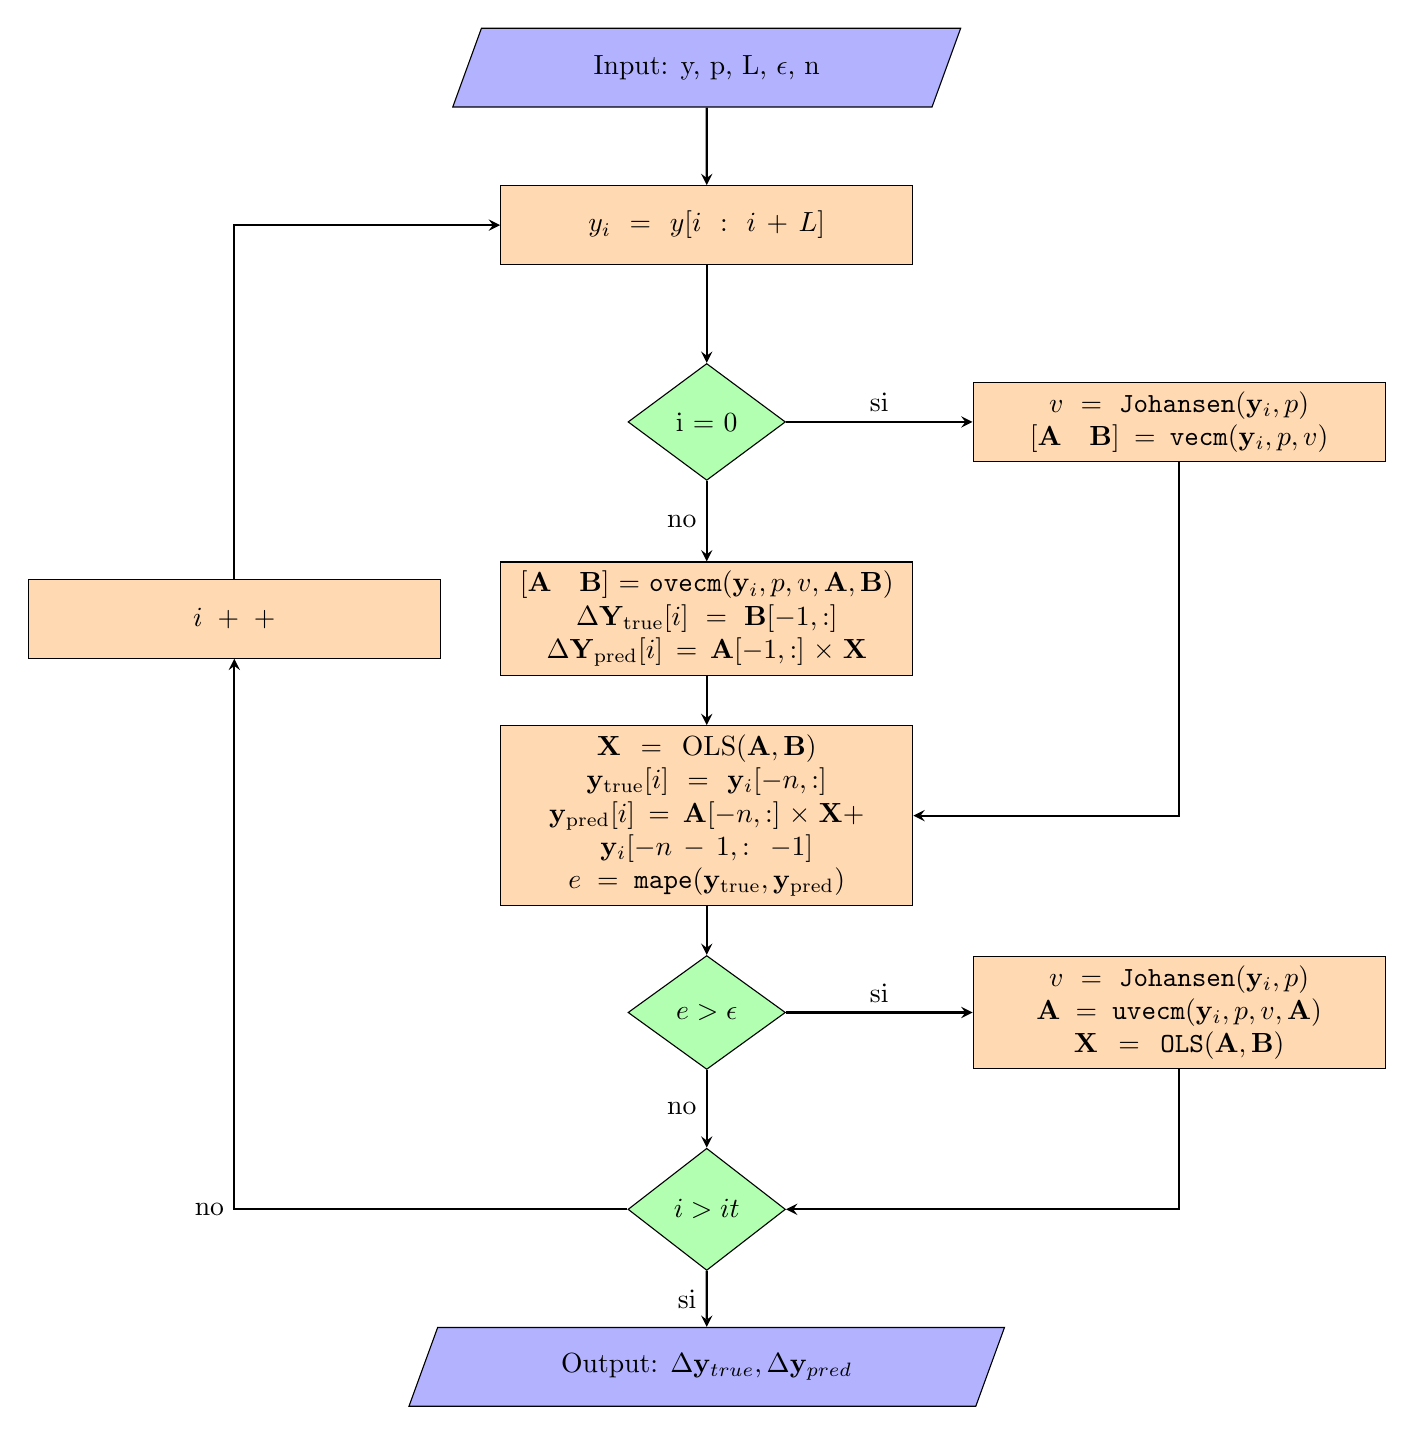
\begin{tikzpicture}[node distance=2cm]
    %\node (start) [startstop] {Start};
    %\node (in1) [io, below of=start] {Input};
    \node (in1) [io] {Input: y, p, L, $\epsilon$, n};
    \node (pro1) [process, below of=in1] {$y_i = y[i:i+L]$};
    \node (dec1) [decision, below of=pro1, yshift=-0.5cm] {i = 0};
    \node (pro2a) [process, below of=dec1, yshift=-0.5cm] {$[\mathbf{A} \quad \mathbf{B}] =\texttt{ovecm}(\mathbf{y}_i,p,v,\mathbf{A},\mathbf{B})$
                                                        $\Delta \mathbf{Y}_{\text{true}}[i] = \mathbf{B}[-1,:]$
                                                        $\Delta \mathbf{Y}_{\text{pred}}[i] = \mathbf{A}[-1,:] \times \mathbf{X}$};

    \node (pro2b) [process, right of=dec1, xshift=4cm] {$v = \texttt{Johansen}(\mathbf{y}_i,p)$ $[\mathbf{A} \quad 
                                                                \mathbf{B}] = \texttt{vecm}(\mathbf{y}_i,p,v)$};
    \node (pro3) [process, below of=pro2a, yshift=-0.5cm] {$\mathbf{X} = \text{OLS} (\mathbf{A},\mathbf{B})$ \\
                                                        $\mathbf{y}_{\text{true}}[i] = \mathbf{y}_i[-n,:]$ \\
                                                        $\mathbf{y}_{\text{pred}}[i] = \mathbf{A}[-n,:] \times \mathbf{X} +$ \\$ \mathbf{y}_i[-n-1,:-1]$ \\
                                                        $e = \texttt{mape}(\mathbf{y}_{\text{true}}, \mathbf{y}_{\text{pred}})$};

    \node (dec2) [decision, below of=pro3, yshift=-0.5cm] { $e > \epsilon $ };

    \node (pro4a) [process, right of=dec2, xshift=4cm] {$v = \texttt{Johansen}(\mathbf{y}_i,p)$ \\
                                                        $\mathbf{A} = \texttt{uvecm}(\mathbf{y}_i,p,v,\mathbf{A})$ \\
                                                        $\mathbf{X} = \texttt{OLS} (\mathbf{A},\mathbf{B})$};

   
    \node (pro5) [process, left of=pro2a, xshift=-4cm] {$ i++ $}; 
   
    \node (dec3) [decision, below of=dec2, yshift=-0.5cm] { $i > it $ };
    
    \node (out1) [io, below of=dec3] {Output: $\Delta \mathbf{y}_{true}, \Delta \mathbf{y}_{pred}$};
    
    %\node (stop) [startstop, below of=out1] {Stop};
    
    %\draw [arrow] (start) -- (in1);
    \draw [arrow] (in1) -- (pro1);
    \draw [arrow] (pro1) -- (dec1);
    \draw [arrow] (dec1) -- node[anchor=east] {no} (pro2a);
    \draw [arrow] (dec1) -- node[anchor=south] {si} (pro2b);
    \draw [arrow] (pro2a) -- (pro3);
    \draw [arrow] (pro2b) |- (pro3);
    \draw [arrow] (pro3) -- (dec2);
    \draw [arrow] (dec2) --  node[anchor=south] {si} (pro4a);
    \draw [arrow] (pro4a) |- (dec3);
    
    \draw [arrow] (dec2) --  node[anchor=east] {no} (dec3);
    \draw [arrow] (dec3.west) -| node[anchor=east] {no} (pro5);
    \draw [arrow] (pro5) |- (pro1);
    \draw [arrow] (dec3) --  node[anchor=east] {si} (out1);
    %\draw [arrow] (out1) -- (stop);
    \end{tikzpicture}
    
    
\section{Results} \label{sec:results}

\subsection{Data} \label{sec:unitroot}
Tests of SLVECM, SLARIMA and our proposal OVECM were carried out using foreign
four exchange data rates: EURUSD, GBPUSD, USDCHF and USDJPY. This data was
collected from the free database Dukascopy which gives access to the Swiss
Foreign Exchange Marketplace ~\cite{Dukascopy2014}.

The reciprocal of the last two rates (CHFUSD, JPYUSD) were used in order to
obtain the same base currency for all rates.  The tests were done using
1-minute frequency from ask prices which corresponded to 1.440 data points per
day from the 11th to the 15th of August 2014.

\subsection{Unit root tests} \label{sec:unitroot}
Before running the tests, we firstly checked if they were I(1) time series
using the Augmented Dickey Fuller (ADF) test.

\begin{table}[h!]
\caption{Unit roots tests}
\label{tab:adf}
\begin{center}
\begin{tabular}{|l|c|c|c|c|c|}
\hline
& \textbf{Statistic} & \textbf{Critical value} & \textbf{Result}\\
\hline
EURUSD          & -0.64 & -1.94 & True       \\
$\Delta$EURUSD & -70.45   & -1.94 & False       \\
GBPUSD          & -0.63   & -1.94 & True          \\
$\Delta$GBPUSD & -54.53   & -1.94 & False       \\
CHFUSD          & -0.88   & -1.94 & True         \\
$\Delta$CHFUSD & -98.98   & -1.94 & False       \\
JPYUSD          & -0.65 & -1.94 & True        \\
$\Delta$JPYUSD & -85.78 & -1.94 & False     \\ 
\hline
\end{tabular}
\end{center}
\end{table}


Table~\ref{tab:adf} shows that all currency rates cannot reject the unit root
test but they rejected it with their first differences. This means that all of
them are I(1) time series and we are allowed to use VECM and therefore OVECM.


\subsection{Parameter selection} \label{sec:paramselection}

In order to set OVECM parameters: windows size $L$ and lag order $p$,
we propose to use several window sizes: $L = 100, 400, 700, 1000$. For every window size $L$ we chose lag order with minimum AIC.

ARIMA parameters were also obtained using AIC.
Parameters optimisation is presented in table~\ref{tab:params}:

\begin{table}[ht]
\caption{Parameters optimisation. VECM order and ARIMA parameters were selected
using AIC.}
\label{tab:params}
\begin{center}
\begin{tabular}{|c|c|c|}
\hline
Windows size $L$ & VECM & ARIMA\\
 $L$ & order $(p)$ & order $(p,d,q)$ \\
\hline
100 & 2 & p=2,d=1,q=1\\
400 & 5 & p=1,d=1,q=1\\
700 & 3 &p=2,d=1,q=1\\
1000 &3 & p=2,d=1,q=1\\
\hline
\end{tabular}
\end{center}
\end{table}

In OVECM we also define a mean\_error variable, which was defined based on the
in-sample MAPEs. Figure \ref{fig:mapes} shows how MAPE moves and how mean\_error
variable help us to decide whether new cointegration vectors are needed.

\begin{figure}[!h]
  \centering
   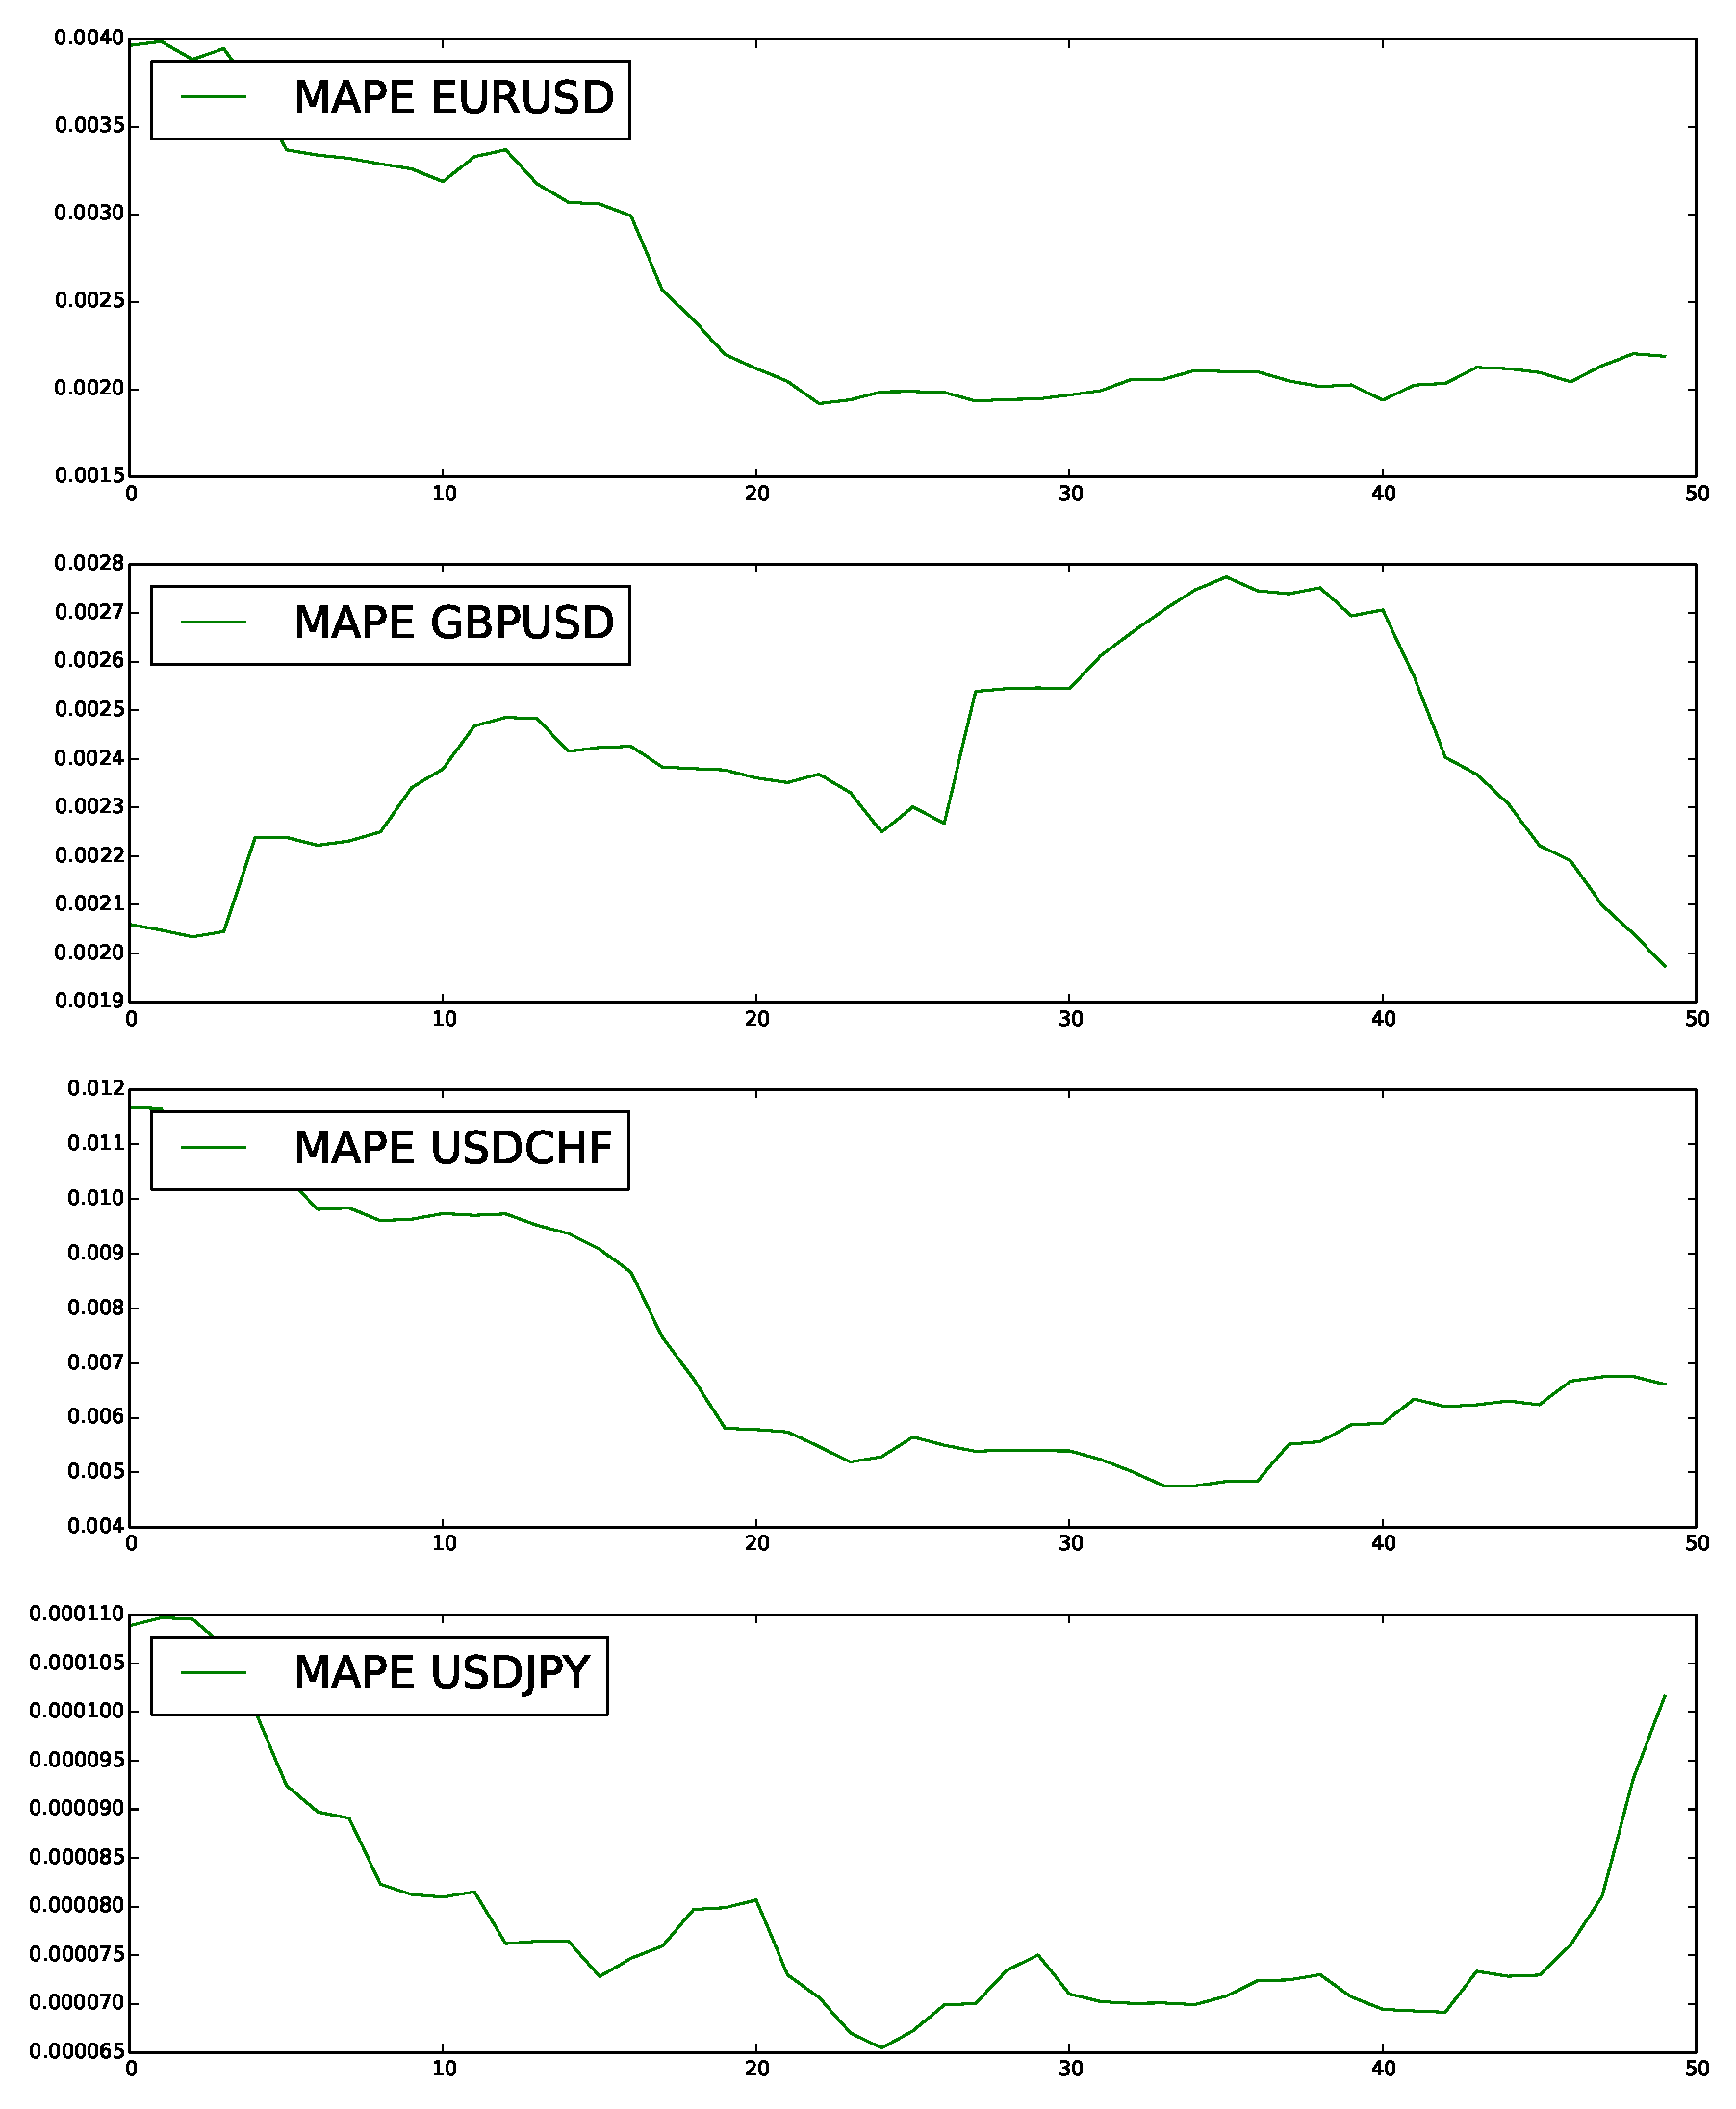
\includegraphics[width = 7.5cm]{img/mapes} 
  \caption{In-sample MAPEs example for 50 minutes. The average of them is
  considered to obtain new cointegration vectors.}
  \label{fig:mapes}
 \end{figure}



\subsection{Execution times} \label{sec:exectimes}
We ran OVECM and SLVECM 400 iterations. SLARIMA execution time is excluded
because its is not comparable with OVECM and SLVECM. SLARIMA was created based
on statsmodels library routine ARIMA.

The execution times are shown in the table~\ref{tab:extimes}.

\begin{table}[h!]
\caption{Execution times}
\label{tab:extimes}
\begin{center}
\begin{tabular}{|l|c|c|c|c|c|}
\hline
& $L$ & order & e  & Time[s] \\
\hline
OVECM & 100 &p=2  & 0      & 2.492\\
OVECM & 100 &p=2  & 0.0026  & 1.606\\
SLVECM & 100 &p=2& -- & 2.100\\
\hline
OVECM & 400 & p=5  & 0      & 3.513\\
OVECM & 400 &p=5  & 0.0041  & 2.569\\
SLVECM & 400 & p=5 & -- & 3.222\\
\hline
OVECM & 700 &p=3  & 0      & 3.296\\
OVECM & 700 &p=3  & 0.0032  & 2.856\\
SLVECM & 700 &p=3 & -- & 3.581\\
\hline
OVECM & 1000 & p=3 & 0      & 4.387\\
OVECM & 1000 & p=3  & 0.0022  & 2.408\\
SLVECM & 1000 & p=3  & -- & 3.609\\
\hline
\end{tabular}
\end{center}
\end{table}

It is clear that execution time depends directly on $L$ and $p$ since they
determine the size of matrix $\mathbf{A}$ and therefore affect the OLS function
execution time.
It is worthy of note that execution time also depends on mean\_error because it
determines how many times OVECM will recalculate cointegration vectors which is
an expensive routine.

Figure~\ref{fig:mapes} shows an example of the in-sample MAPE for 50 iterations.
When the average of the in-sample MAPEs is above mean\_error new cointegration
vectors are obtained. In consequence, OVECM performance increases when
mean\_error increases. However, this could affect accuracy, but
table~\ref{tab:stats} shows that using an appropriate mean\_error doesn't affect
accuracy considerable. 

\subsection{Performance accuracy} \label{sec:performacc}

Table~\ref{tab:stats} shows in-sample and out-of-sample performance measures:
MAPE, MAE and RMSE for OVECM, SLVECM and SLARIMA. Test were done using the
parameters defined in table \ref{tab:params}.  We can see that OVECM has very
similar performance than SLVECM and this support the theory that cointegration
vectors vary little in time. Moreover, OVECM also out performed SLARIMA based on
these three performance measures. 


\begin{table*}[ht!]
\caption{Model measures}
\label{tab:stats}
\begin{center}
\begin{tabular}{|l|l|c|c|c|c|c|c|c|c|}
\hline
\multicolumn{4}{|c|}{Model} & \multicolumn{3}{|c|}{In-sample} &
\multicolumn{3}{|c|}{Out-of-sample} \\ 
\hline
\hline
Method & $L$ & Parameters & e & 
MAPE & MAE& RMSE& 
MAPE & MAE& RMSE \\
\hline
 OVECM  &   100  &  P=2& 0.0026  &  0.00263&  0.00085&  0.00114&  0.00309&  0.00094&  0.00131\\
 OVECM  &   400  &  P=5& 0.0041  &  0.00378&  0.00095&  0.00127&  0.00419&  0.00103&  0.00143\\
 OVECM  &   700  &  P=3& 0.0032  &  0.00323&  0.00099&  0.00130&  0.00322&  0.00097&  0.00132\\
 OVECM  &   1000 &  P=3& 0.0022  &  
 \textbf{0.00175}&  \textbf{0.00062}&  \textbf{0.00087} &  
 \textbf{0.00172}&  \textbf{0.00061}&  \textbf{0.00090}\\
\hline
 SLVECM  &   100 &  P=2& -  &  0.00262&  0.00085&  0.00113&  0.00310&  0.00095&  0.00132\\
 SLVECM  &   400 &  P=5& -  &  0.00375&  0.00095&  0.00126&  0.00419&  0.00103&  0.00143\\
 SLVECM  &   700 &  P=3& -  &  0.00324&  0.00099&  0.00130&  0.00322&  0.00098&  0.00132\\
 SLVECM  &   1000 &  P=3& -  &  
 \textbf{0.00174}&  \textbf{0.00061}&  \textbf{0.00087}&  
 \textbf{0.00172}&  \textbf{0.00061}&  \textbf{0.00090}\\
\hline
SLARIMA & 100  &p=2, d=1, q=1 & - & 0.00285  &  0.00110  &  0.00308  &  0.00312  &0.00098  &  0.00144 \\
SLARIMA & 400  &p=1, d=1, q=1 & - & 0.00377  &  0.00101  &  0.00128  &  0.00418 & 0.00106 & 0.00145 \\
SLARIMA & 700  &p=2, d=1, q=1 & - & 0.00329  &  0.00102  &  0.00136  &  0.00324  & 0.00097  &  0.00133 \\
SLARIMA & 1000 &p=2, d=1, q=1 & - & \textbf{0.00281}  & \textbf{0.00074}  &  \textbf{0.00105}  &  \textbf{0.00177} & \textbf{0.00063}  &  \textbf{0.00092} \\
\hline
\end{tabular}
\end{center}
\end{table*}

We can also notice that in-sample performance in OVECM and SLVECM is related
with the out-of-sample performance.  This differs with SLARIMA which models with
good in-sample performance are not necessarily good out-of-sample models.
Moreover OVECM outperformed SLARIMA using the same window size.

Figure ~\ref{fig:accuracy} shows the out-of-sample forecasts made by our
proposal OVECM with the best parameters found based on table~\ref{tab:stats}
which follows the time series very well.  

\begin{figure}[h]
  \vspace{-0.2cm}
  \centering
   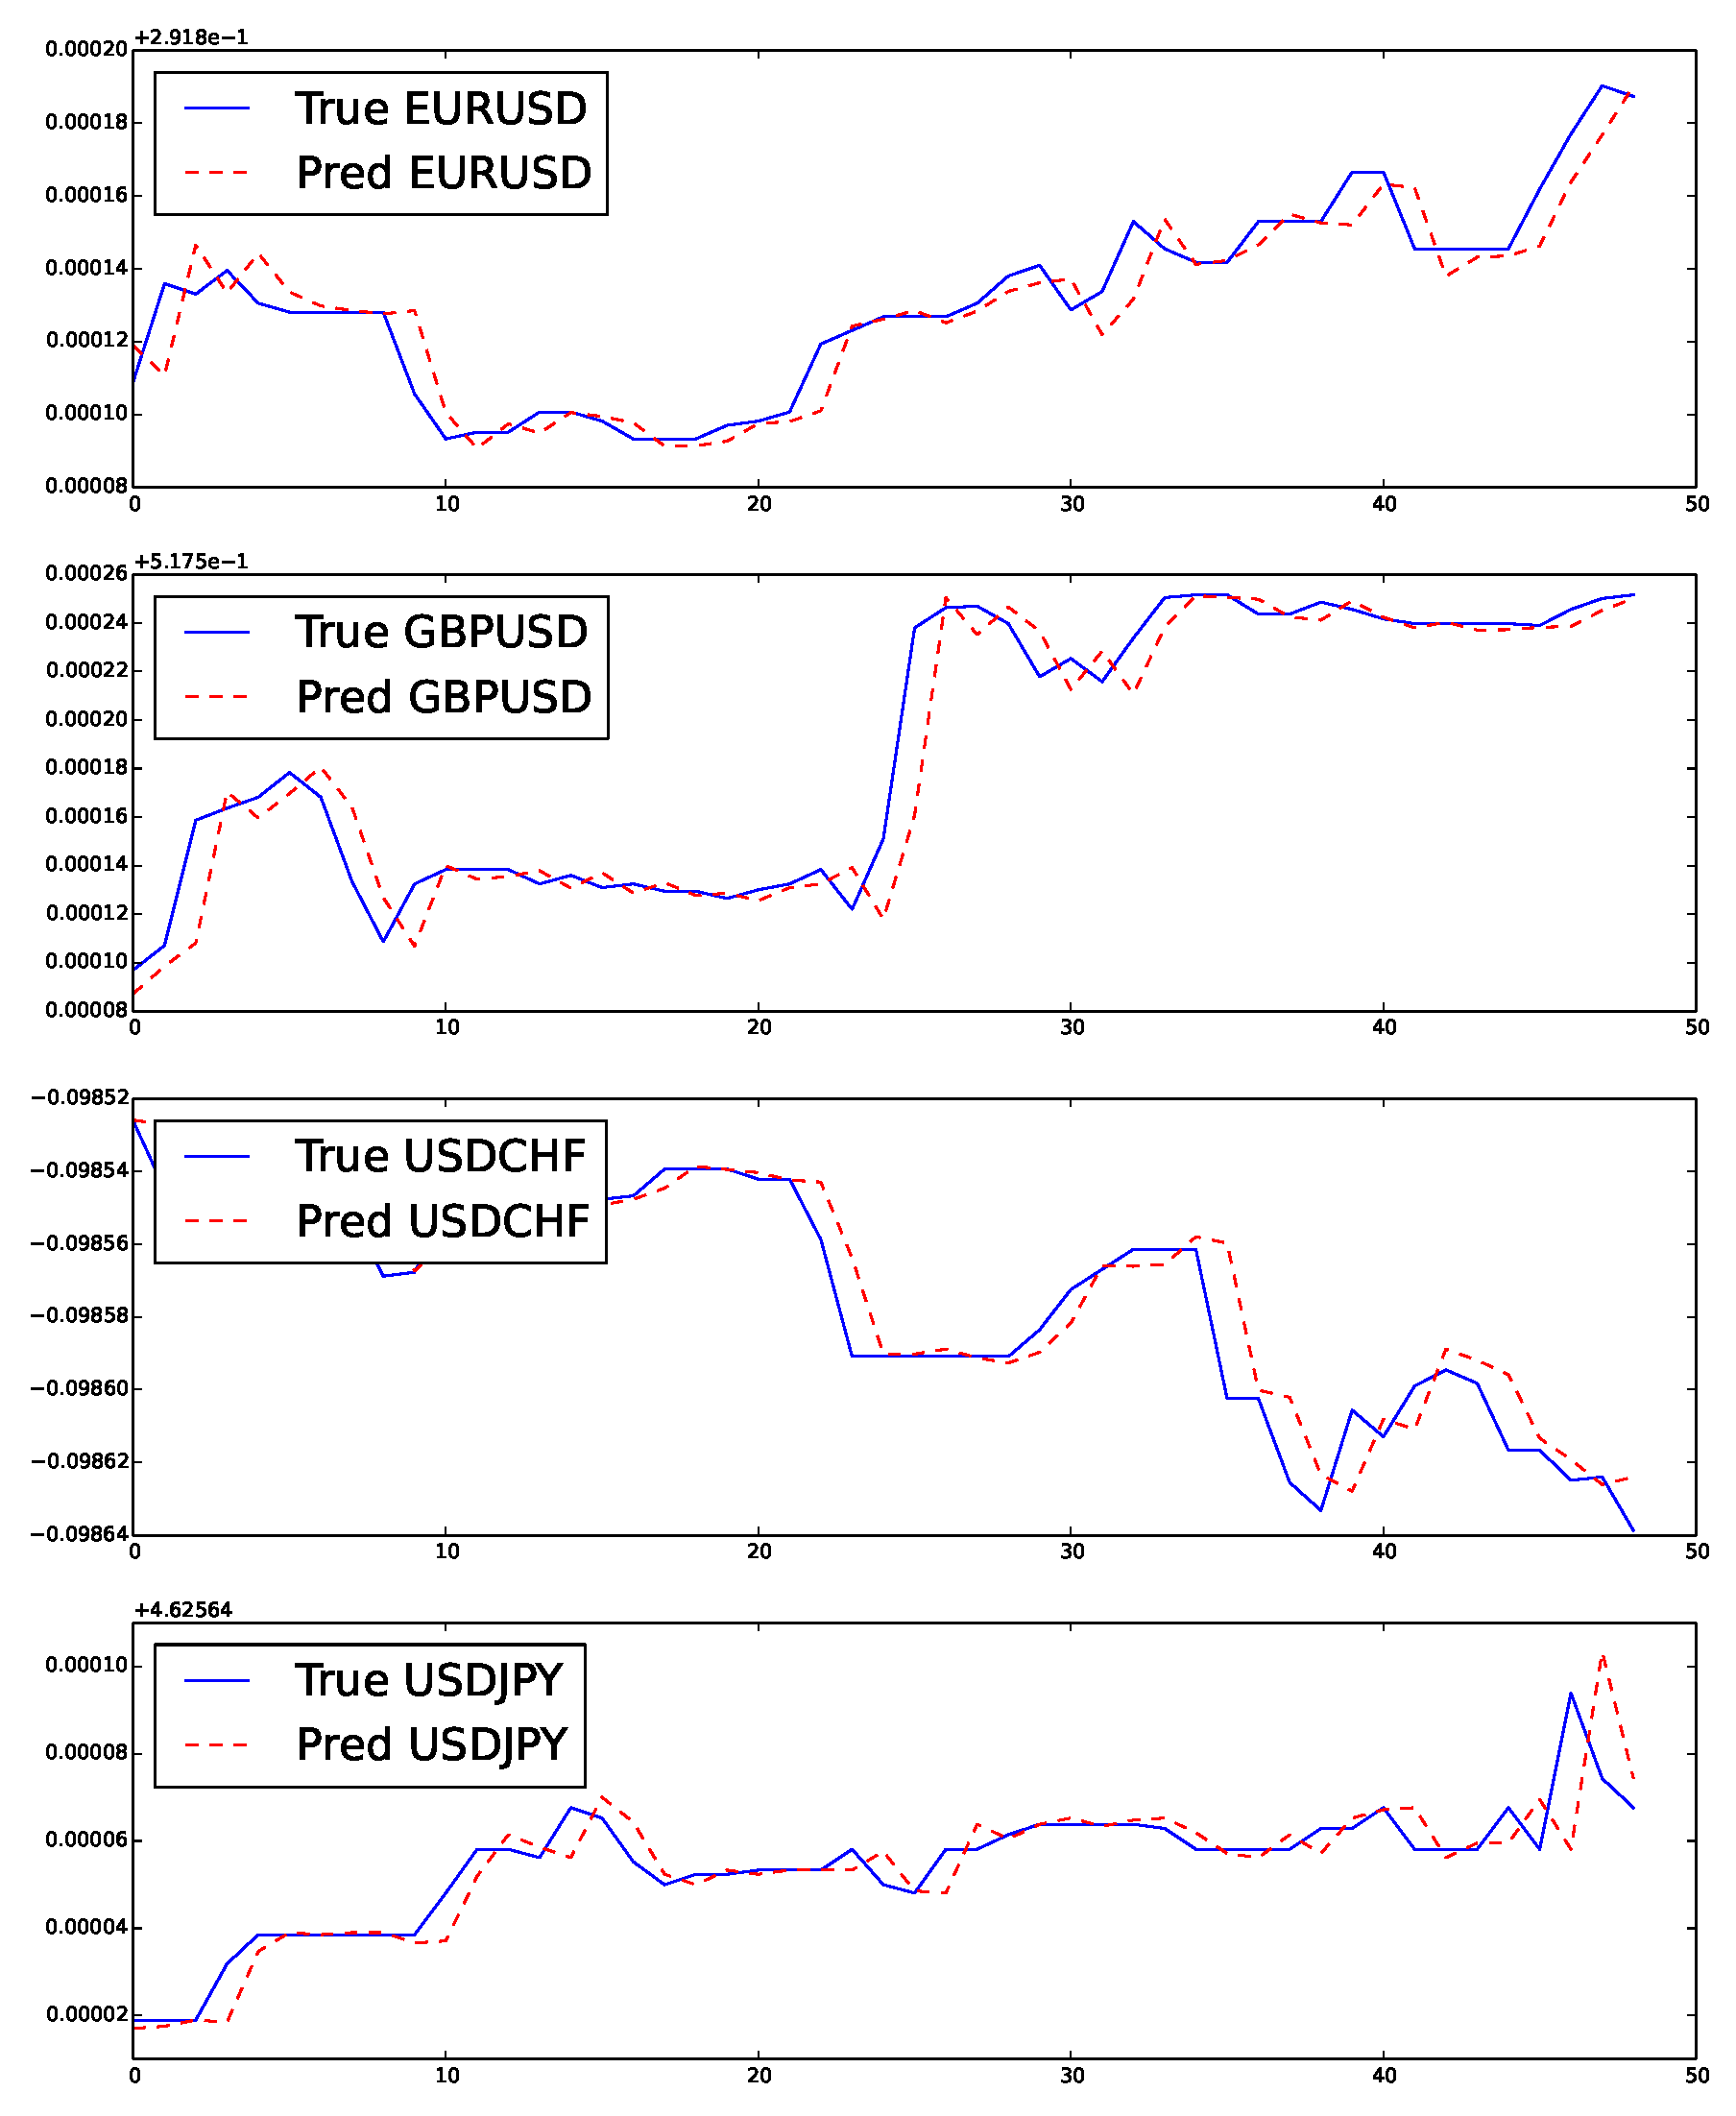
\includegraphics[width = 7.5cm]{img/accuracy} 
  \caption{OVECM forecasting accuracy example for 50 minutes using $L = 1000$ and $p =3$}
  \label{fig:accuracy}
 \end{figure}



\section{Conclusions} \label{sec:conclusions}

A new online vector error correction method was presented. 
We have shown that our proposed OVECM considerably reduces execution times
without compromising solution accuracy.  OVECM was compared with VECM and ARIMA
with the same sliding window sizes and OVECM outperformed both in terms of
execution time. Traditional VECM slightly outperformed our proposal but the
OVECM execution time is lower.
This reduction of execution time is mainly because OVECM avoids the cointegration vector
calculation using the Johansen method. The condition for getting new vectors is
given by the mean\_error variable which controls how many times the Johansen method is
called. Additionally, OVECM introduces matrix optimization in order to get the
new model in an iterative way.
We could see that our algorithm took much less than a minute at every
step. This means that it could also be used with higher frequency data and would
still provide responses before new data arrives.  

For future study, it would be interesting to improve the out-of-sample forecast
by considering more explicative variables, to increase window sizes or trying new
conditions to obtain new cointegration vectors. 

Since OVECM is an online algorithm which optimizes processing time, it could be
used by investors as an input for strategy robots. Moreover, some technical
analysis methods could be based on its output. 




\chapter{Adaptive parallel algorithm for VECM}

VECM parameters are those which maximise cointegration relations in the past. However, this search is computationally expensive since the Johansen
method~\cite{johansen1995} is used, which is of order $O(n^3)$. We propose
to parallelise this search in order to get new parameters at every iteration. 

\vspace{0.5cm} 

\section{Introduction}
Both VECM and VAR model parameters are obtained using ordinary least squares
(OLS) method \cite{golub1980}. Since OLS involves many calculations, the parameter estimation
method is computationally expensive when the number of past values and
observations increases. Moreover, obtaining cointegration vectors 
is also an expensive routine because of the use of the Johansen method.

Model effectiveness is focused on out-of-sample forecast rather than in-sample
fitting. This criterion allows our proposal AVECM prediction capability to be
expressed rather than just explaining data history.

The forecast capability of our method was measured using MAPE, MAE and
RMSE \cite{armstrong1992}. Tests were run using four currency rates: Euro (EUR) to
United States Dollar (USD) (EURUSD), British Pound (GBP) to USD (GBPUSD), USD to Swiss
Franc (CHF) (USDCHF) and USD to Japanese Yen (JPY) (USDJPY) with a 10-seconds frequency.

\def\rot#1{{\color{red}{#1}}}
\def\gruen#1{{\color{green}{#1}}}
\def\blau#1{{\color{blue}{#1}}}


\section{Background}
\label{sec:background}

VECM is obtained re-writing equation (\ref{eq:var}) in terms of the new
variable $\Delta\mathbf{y}_t=\mathbf{y}_t-\mathbf{y}_{t-1}$.
The VECM model, expressed in terms those differences, takes the form:
\begin{equation}\label{eq:vec}
\Delta \mathbf{y}_t 
= \boldsymbol{\Omega}\,\mathbf{y}_{t-1}
  + \sum_{i=1}^{p-1} \boldsymbol{\Phi}_i^*\,\Delta\mathbf{y}_{t-i}
  + \mathbf{c} + \boldsymbol{\epsilon}_t\,,
\end{equation}
\noindent
where the coefficients matrices $\boldsymbol{\Phi}_i^*$ and 
$\boldsymbol{\Omega}$, expressed in terms of the matrices
$\boldsymbol{\Phi}_i$ of (\ref{eq:var}), are:
\begin{align*}
\boldsymbol{\Phi}_i^* 
&:= -\sum_{j=i+1}^{p}\boldsymbol{\Phi}_j\,, \\
\boldsymbol{\Omega}
&:= -\left( \mathbb{I} - \boldsymbol{\Phi}_1 - \dots 
    - \boldsymbol{\phi}_p \right)\,. 
\end{align*}
The following well known properties of the matrix $\boldsymbol{\Omega}$
\cite{johansen1995} will be useful in the sequel:
\begin{itemize}
\item
If $\boldsymbol{\Omega} = \mathbf{0}$, there is no cointegration.
\item 
If $rank(\boldsymbol{\Omega})=l$, i.e., if $\boldsymbol{\Omega}$ has
full rank, then the time series are not I(1) but stationary.
\item
If $rank(\boldsymbol{\Omega})=r$, $0<r<l$, then there is cointegration
and the matrix $\boldsymbol{\Omega}$ can be expressed as
$\boldsymbol{\Omega}=\boldsymbol{\alpha\beta}^\top$, where $\boldsymbol{\alpha}$
and $\boldsymbol{\beta}$ are
$l\times r$ matrices and
$\text{rank}(\boldsymbol{\alpha})=\text{rank}(\boldsymbol{\beta})=r$.
\item
The columns of $\boldsymbol{\beta}$ contains the cointegration vectors and the rows of
$\boldsymbol{\alpha}$ correspond with the adjusted vectors. 
$\boldsymbol{\beta}$ is obtained by Johansen procedure~\cite{johansen1988},
whereas $\boldsymbol{\alpha}$ has to be determined as a variable in the VECM.
\end{itemize}

If cointegration exists, then equation (\ref{eq:vec}) can be written
as follows:
\begin{equation}\label{eq:vecfull}
\Delta\mathbf{y}_t 
= \boldsymbol{\alpha\beta}^\top\mathbf{y}_{t-1} 
  + \sum_{i=1}^{p-1}\boldsymbol{\Phi}_i^*\,\Delta\mathbf{y}_{t-i}
  + \mathbf{c} + \boldsymbol{\epsilon}_t\,,
\end{equation}
\noindent
which is a VAR model but for time series differences.

Transposing each equation of the system (\ref{eq:vecfull}) we can write
the VECM($p$) model in block-matrix form as:
\begin{equation}\label{eq:vareq}
\mathbf{B} = 
\mathbf{A} \mathbf{X} + 
\mathbf{E} \, , 
\end{equation}
%
\noindent where $\mathbf{B}$ dimension is $((N-p)\times l)$, $\mathbf{A}$
dimension is $((N-p)\times(r+(p-1)l +1))$, $\mathbf{X}$ dimension is $((r+(p-1)l
+1)\times l)$ and $\mathbf{E}$ dimension is $((N-p)\times l)$:
%
\begin{alignat}{3}
\mathbf{B}
&= \begin{bmatrix}
   \Delta\mathbf{y}_{p+1}^\top \\
   \Delta\mathbf{y}_{p+2}^\top \\
   \vdots \\
   \Delta\mathbf{y}_N^\top
   \end{bmatrix}
&\quad
\mathbf{X}
&= \begin{bmatrix}
   \boldsymbol{\alpha}^\top \\
   \boldsymbol{\Phi}_1^{*\top} \\
   \boldsymbol{\Phi}_2^{*\top} \\
   \vdots \\
   \boldsymbol{\Phi}_{p-1}^{*\top} \\
   \mathbf{c}^\top
   \end{bmatrix}
&\quad
\mathbf{E}
&= \begin{bmatrix}
   \boldsymbol{\epsilon}_{p+1}^\top \\
   \boldsymbol{\epsilon}_{p+2}^\top \\
   \vdots \\
   \boldsymbol{\epsilon}_N^\top \\
   \end{bmatrix}
\end{alignat}
\noindent and 
\begin{align}
\mathbf{A} 
&= \begin{pmat}[{....|}]
   \mathbf{y}_p^\top \boldsymbol{\beta} & \Delta \mathbf{y}_p^\top & \Delta\mathbf{y}_{p-1}^\top & \dots 
                    & \Delta\mathbf{y}_2^\top & 1 \cr
   \mathbf{y}_{p+1}^\top  \boldsymbol{\beta} &\Delta\mathbf{y}_{p+1}^\top & \Delta\mathbf{y}_p^\top & \dots
                       & \Delta\mathbf{y}_3^\top & 1 \cr
   \vdots & \vdots & \vdots & \ddots & \vdots & \vdots \cr
   \mathbf{y}_{N-1}^\top  \boldsymbol{\beta} &\Delta\mathbf{y}_{N-1}^\top & \Delta\mathbf{y}_{N-2}^\top & \dots 
                       & \Delta\mathbf{y}_{N-p-1}^\top & 1 \cr
   \end{pmat}\, .
\end{align}
Taking into account the error term $\mathbf{E}$, equation~(\ref{eq:vareq}) 
can be solved with respect to $\mathbf{X}$ using the ordinary least
squares estimation.

\section{Motivation} \label{sec:proposal}

Cointegration vectors can be found applying the Johansen method which uses a
sample of the last historical data. However, one of the main limitations of this
methodology is that it assumes cointegration vectors do not change in time.
In fact, the long-run relationships between the time series might change due to
several economic factors that can lead to structural breaks in the cointegrating
relation \cite{gregoryETal1996}. 
Experiments show that cointegration depends on the amount $L$ of historical data
considered, and how many lags $p$ we use.

Figure~\ref{fig:hists} shows the number $r$ of cointegration vectors given by
the Johansen method for different values of the parameters $L$ and $p$, using
four currencies data, i.e., $l=4$, and considering 1000 iterations $it$.
We know that when there is no cointegration vectors, i.e $r=0$, 
there is no cointegration. In the same way, when $r=l$ reveals that no process is I(1) but,
instead, they are all stationary.
The interesting cases of cointegration are those, where $r$ lies strictly
between $0$ and $l$, i.e. $0<r<l$, 

Experiments were run with data starting at 9:00 GMT of the 11th of August 2014,
which corresponds to the opening of the New York financial market.

\begin{figure}[!h]
  %\vspace{-0.8cm}
  \centering
  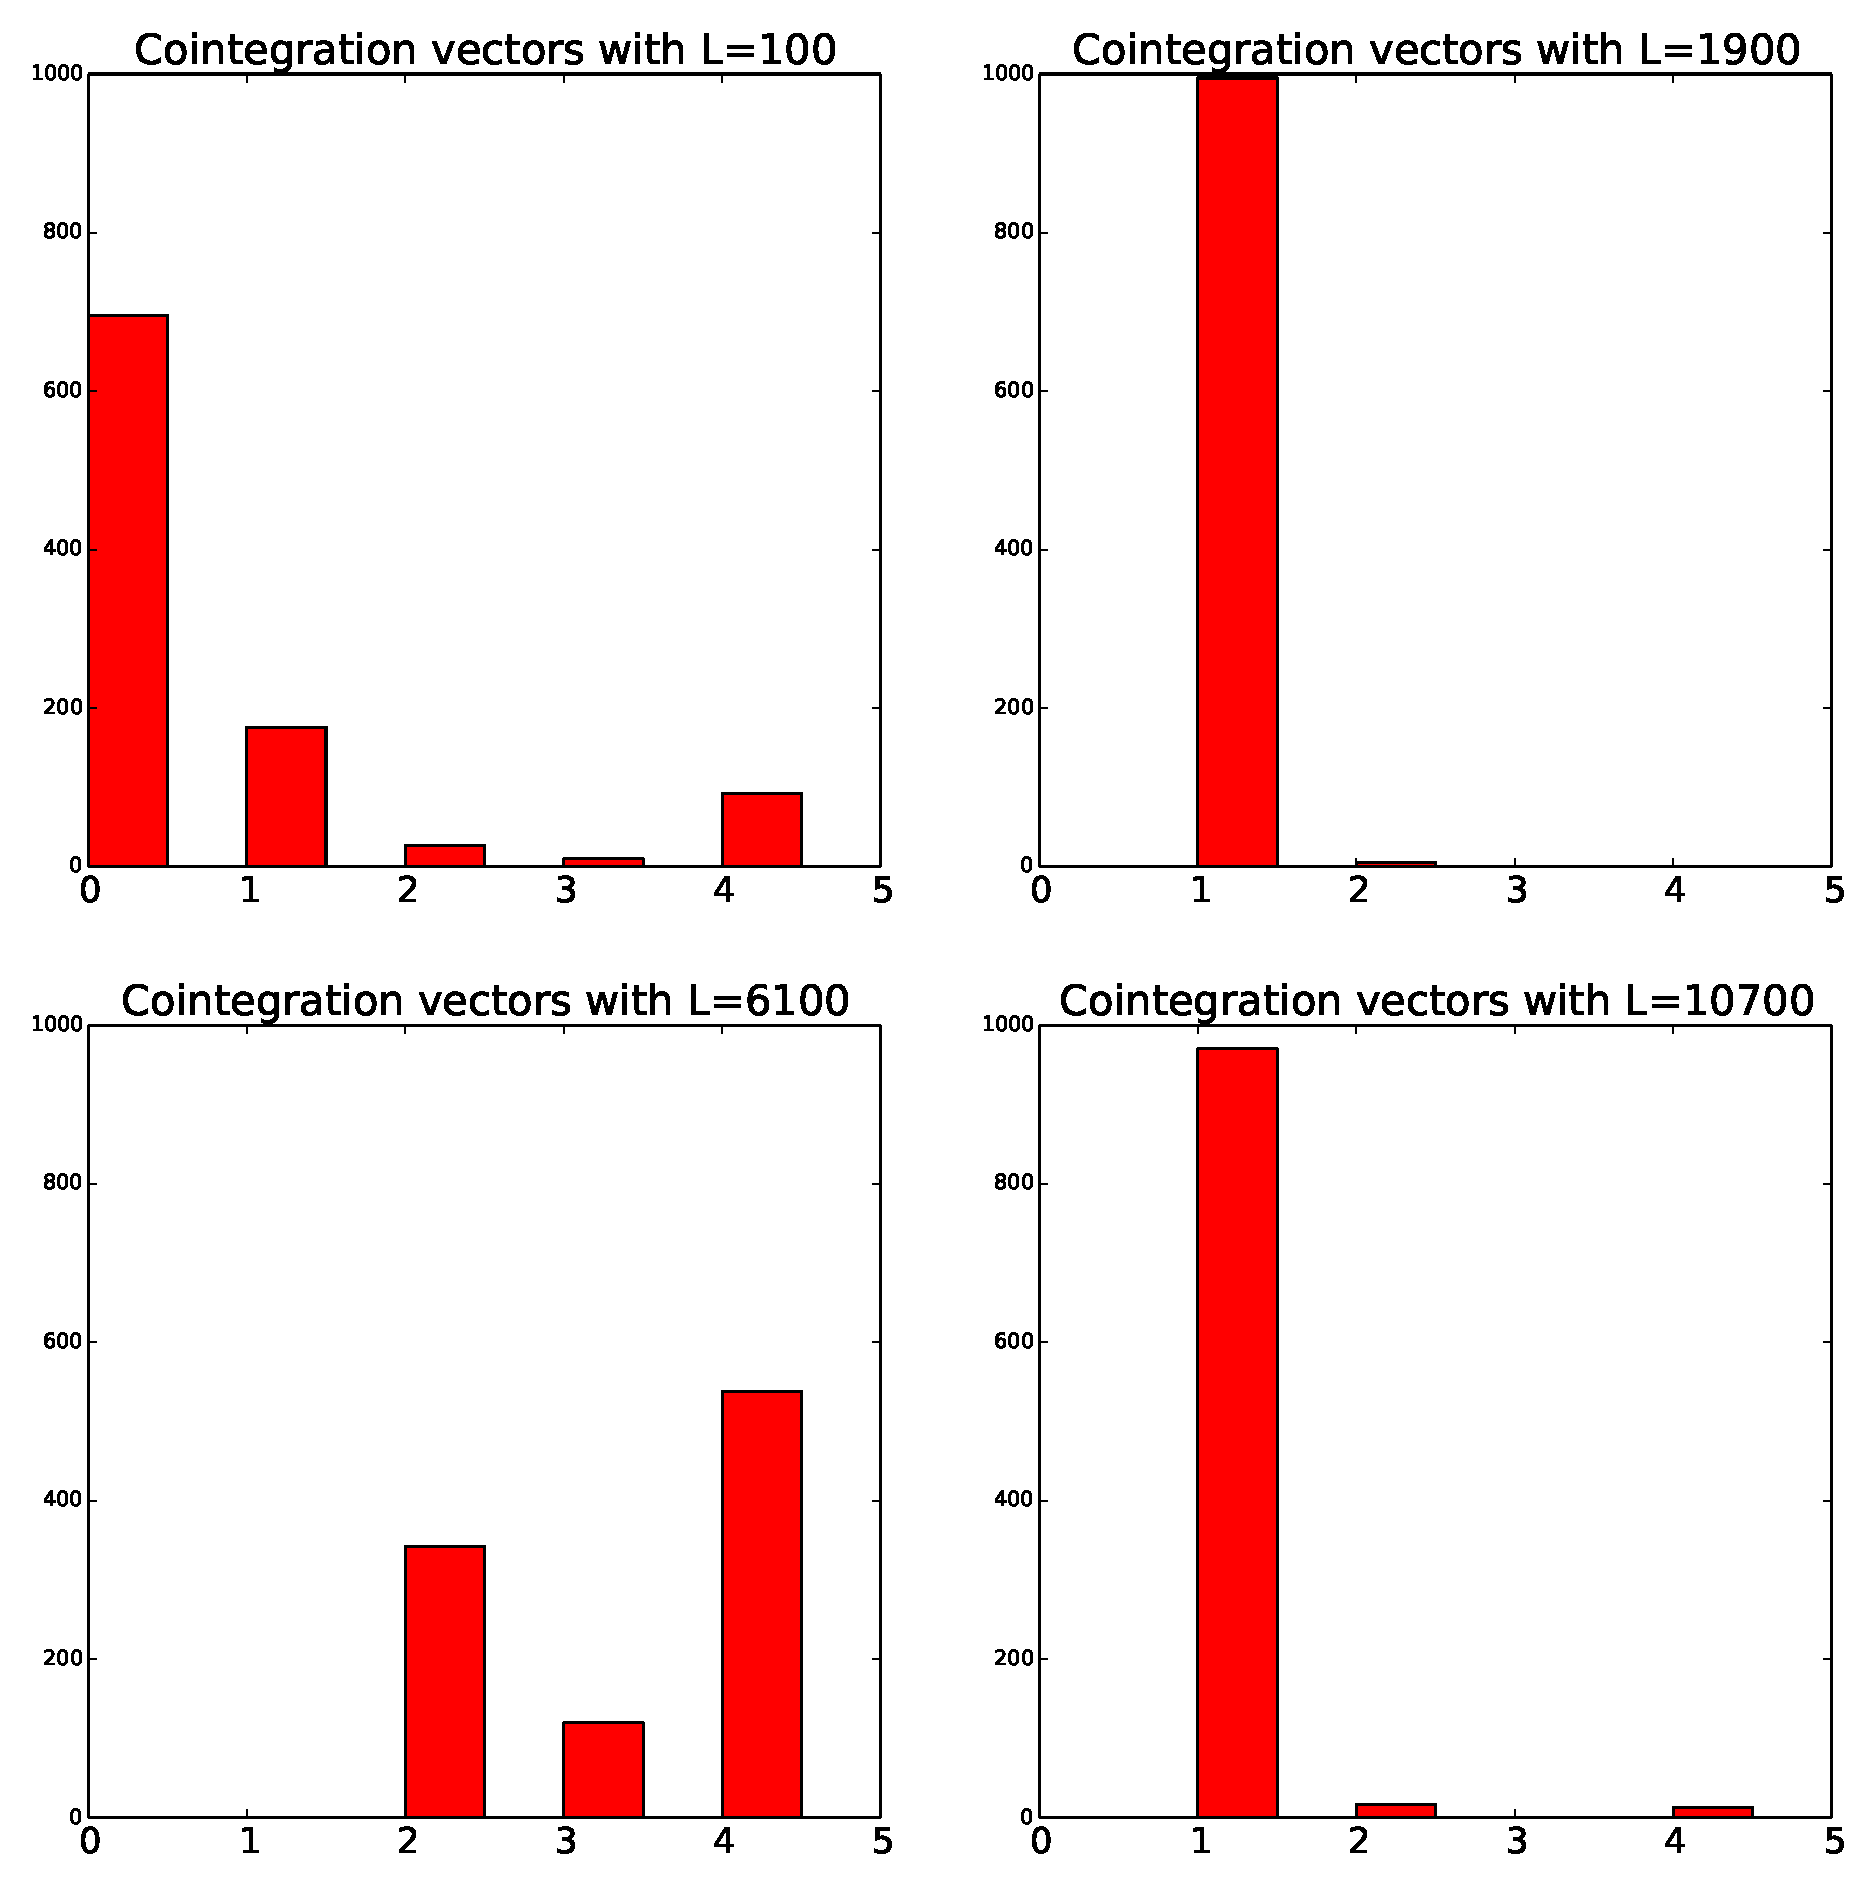
\includegraphics[width=\textwidth]{img/histCointVectors}
  \caption{Histogram of the number of cointegration vectors using $p=1$. Four
  possible values for $L$ are shown (100, 1900, 6100 and 10700).
  In the cases of $L=100$ and $L=6100$, most of the time there is little
  cointegration (0 or 4 cointegration vectors). However, for $L=1900$ and
  $L=10700$ significant cointegration is found.}
  \label{fig:hists}
\end{figure}

\begin{figure}[!h]
  %\vspace{-0.8cm}
  \centering
  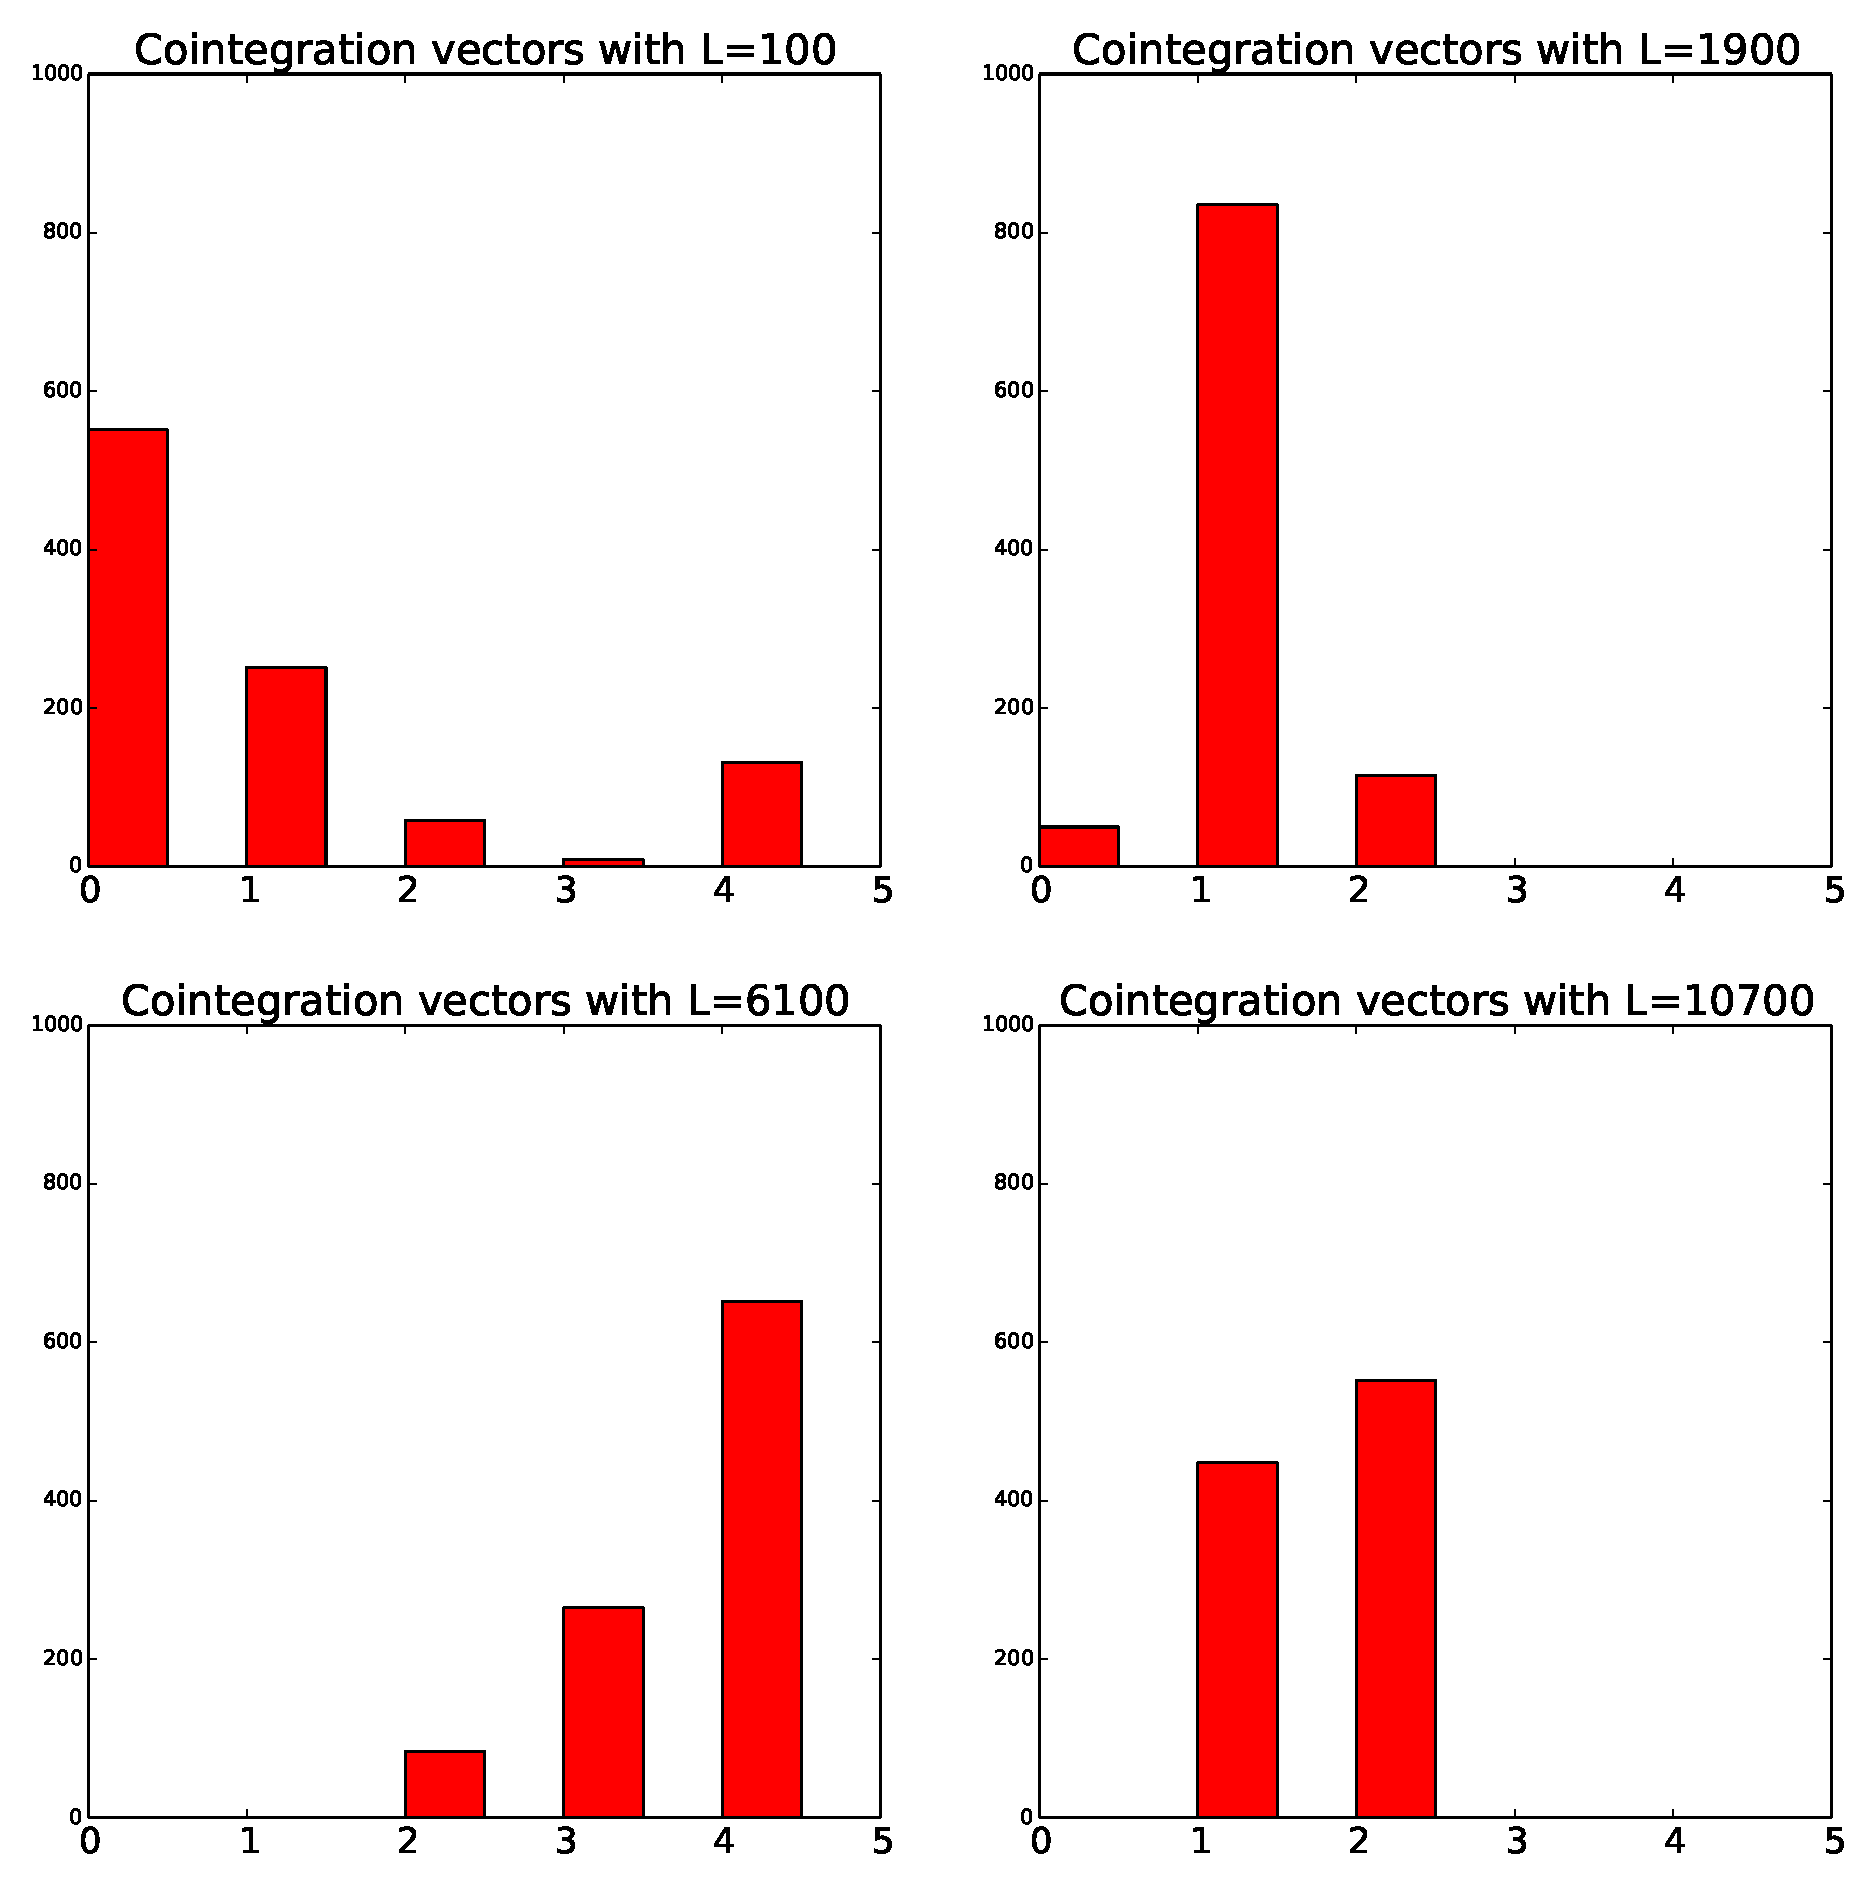
\includegraphics[width=\textwidth]{img/histCointVectorsp5}
  \caption{Histogram of the number of cointegration vectors using $p=5$. 
   Despite the change in the distribution of cointegration vectors, 
   the percentage of cointegration is nearly the same as in the case $p=1$. 
   For example, for $L=10700$ the sum of 1 and 2 number of cointegration
   vectors is very similar to 1 cointegration vector for the case $L=10700$
   in figure \ref{fig:hists}.}
   \label{fig:histsp5}
\end{figure}

The same experiments, using now $p=5$, were carried out in order to see the
effect on the number of cointegration vectors found. 
Figure~\ref{fig:histsp5} shows that, despite the change in the distribution
of the number of cointegration vectors, the sum of their number with $0<r<4$,
remain nearly the same. 
Therefore we can say that the number of lags doesn't significantly affect
the extent of cointegration found.

In order to measure the extent of cointegration, we introduce a
{\em percentage of cointegration\/} as following:
\begin{equation} \label{eq:pcoint}
PC = 
\frac{\#\{ it \mid \text{$it$ has $r$ c.v. with $0<r<l$}\}}
     {\#it}\times 100
\end{equation}
where c.v. stands for cointegration vectors and $it$ is the number of iterations.

The goal of our next experiment was to find a relation between this ratio
$PC$ and the performance of the accuracy measure MAPE (see equation 
\ref{eq:MAPE}). 
The experiments suggest that there is indeed a relation between the $PC$ ratio
and MAPE.
Figure~\ref{fig:cointvsmape} shows that MAPE rapidly decreases with increasing
$PC$.

\begin{figure}[!h]
  %\vspace{-0.8cm}
  \centering
  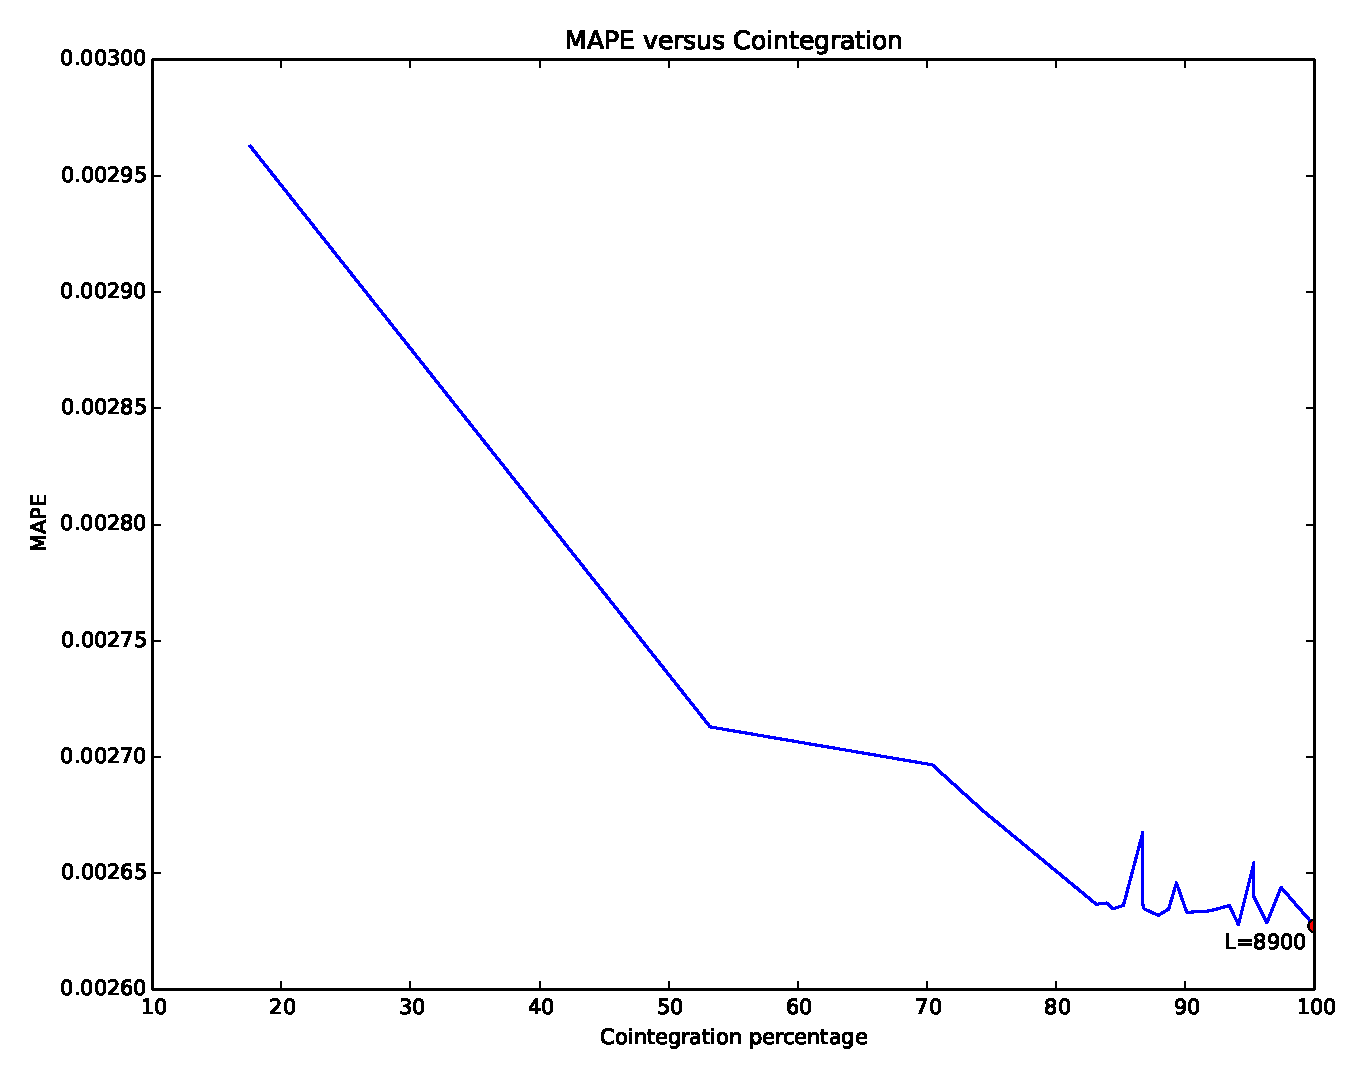
\includegraphics[width=\textwidth]{img/MAPEvsCoint-offset21600-p-2-freq-10s}
  \caption{MAPE versus percentage of cointegration. MAPE was obtained from 1000
  iterations considering several possible $L=[100,10000,400]$ and $p=[1,5]$.
  Best $L$ found was 8900.}
  \label{fig:cointvsmape}
\end{figure}

From these results we observe that cointegration changes with different values
for $L$ and $p$ and also that better cointegration percentage leads to better
accuracy performance.
Therefore we propose to choose best $L$ and $p$ parameters determined at every
step. 
The criterion for choosing $L$ and $p$ is to maximise the percentage of
cointegration $PC$ considering a number of past iterations $it$.

Algorithm ~\ref{alg:AVECM} summarises our proposal. 
The function {\bf get\_best\_params} makes a grid search on the two vector
lists $Ls$ and $ps$ and returns the parameters $L$ and $p$ which maximise
the percentage of cointegration $PC$ (see equation~\ref{eq:pcoint}) for a
pre-defined number of iterations.
Since this search is computational expensive, the number of cointegration
vectors at each iteration is computed in parallel, thus ensuring a response
before new data is available. 
This parallel routine also allows to refine our grid search leading to obtain
improved forecasting performance.
After that optimum $L$ and $p$ parameters are found, VECM is built and used
to forecast next data.

\begin{algorithm}[ht]
\begin{algorithmic}[1]
\REQUIRE $\,$ \\
$\mathbf{y}$: matrix with $N$ input vectors and $l$ time series\\
$ps$: vector with the number of past values range \\
$Ls$: vector with window sizes range ($L<N$) \\
$outit$: Number of out-of-sample iterations($outit < N-L$)
$it$: Number of iterations of testing (in-sample)\\
$of$: Starting point of Testing \\
\ENSURE  $\,$ \\
$\{ \mathbf{y}_{\text{pred}}[1],\dots,\mathbf{y}_{\text{pred}}[N-L]\}$: model predictions 
\FOR { $i =of$ to $of + outit$ }
   \STATE $\mathbf{Y} \gets \mathbf{y}[i-\texttt{max}(Ls):i]$
    \STATE $L,p \gets
    \texttt{get\_best\_params}(Ls,ps,it,Y)$
    \STATE $\mathbf{y}_i \gets \mathbf{y}[i-L:i]$
        \STATE $model = VECM(\mathbf{y}_i, p)$
        \STATE $\mathbf{y}_{\text{pred}}[i] = model.predict()$
\ENDFOR
\end{algorithmic}
\caption{AVECM: Adaptive VECM.}
\label{alg:AVECM}
\end{algorithm}

%
%
%\subsection{Evaluation methods} \label{sec:evaluation}
%
%Forecast performance was evaluated using different methods. We chose three
%measures that are frequently used:
%\begin{description}
%\item
%{\bf MAPE}, Mean Average Percent Error, which presents forecast errors as a
%percentage:
%\begin{equation}\label{eq:MAPE}
%\text{MAPE} = \frac{1}{N} \sum_{t=1}^{N} 
%\frac{\left|\mathbf{y}_t-\hat{\mathbf{y}}_t\right|}{\left|\mathbf{y}_t\right|}
% \times 100 
%\end{equation}
%\item
%{\bf MAE}, Mean Average Error, which measures the distance between forecasts and the
%true value.
%\begin{equation}\label{eq:MAE}
%\text{MAE} = \frac{1}{N} \sum_{t=1}^{N} 
%\left| 
%\mathbf{y}_t-\hat{\mathbf{y}}_t
%\right| 
%\end{equation}
%\item
%{\bf RMSE}, Root Mean Square Error, also measures the distance between forecasts
%and the true values but, unlike MAE, large deviations from the true value have a
%large impact on RMSE due to squaring forecast error.
%\begin{equation}\label{eq:RMSE}
%\text{RMSE} = \sqrt{
%\frac{\displaystyle \sum_{t=1}^{N} (\mathbf{y}_t-\hat{\mathbf{y}}_t)^2}{N}}
%\end{equation}
%\end{description}
%
%
%
\section{Experimental results}
\label{sec:results}
\subsection{Data} \label{sec:unitroot}
AVECM tests were carried out using four foreign exchange rates all related to
USD: EURUSD, GBPUSD, USDCHF and USDJPY. This data was collected from the free
database Dukascopy which gives access to the Swiss Foreign Exchange marketplace
~\cite{Dukascopy2014}.

The tests were done using 10-seconds frequency from ask prices which
corresponded to 8640 data points per day from the 11th to the 15th of August
2014. Since data datetimes were in GMT, opening market times for London, New
York, Sidney and Tokyo corresponded with data points 1440, 3240, 6120 and 6840
respectively. Our tests were made considering two hours after the opening time
of the 13th of August. Therefore, in order to obtain these times, we added 2
days and 2 hours to all the opening times ($2\times 8640 + 2 \times 360$) to obtain:
19440, 21240, 24120 and 24840. We called offset to these times in
table~\ref{tab:stats}, which allowed us to obtain performance at different
times of the day.

\subsection{Unit root tests} \label{sec:unitroot}
Before running the tests, we firstly checked whether the time series were
I(1) using the Augmented Dickey Fuller (ADF) test at 95\% significance level.
Table~\ref{tab:adf} shows that all currency rates cannot reject the unit root
test but they rejected it with their first differences. This means that all of
them are I(1) time series and we are allowed to use VECM and therefore AVECM.

\begin{table}[h!]
\begin{center}
\begin{tabular}{|l|c|c|c|c|c|}
\hline
& \textbf{Statistic} & \textbf{Critical value} & \textbf{Result}\\
\hline
EURUSD          &  -0.05398   & -1.94101 & True       \\
$\Delta$ EURUSD & -89.12344   & -1.94101 & False       \\
GBPUSD          &  -0.88208   & -1.94101 & True          \\
$\Delta$ GBPUSD & -82.56501   & -1.94101 & False       \\
CHFUSD          & -0.49941    & -1.94101 & True         \\
$\Delta$ CHFUSD & -74.21940   & -1.94101 & False       \\
JPYUSD          &  0.36721    & -1.94101 & True        \\
$\Delta$ JPYUSD & -101.15589  & -1.94101 & False     \\ 
\hline
\end{tabular}
\end{center}
\caption{Unit roots tests for EURUSD, GBPUSD, USDCHF and USDJPY at 10-seconds
frequency.}
\label{tab:adf}
\end{table}


\section{Parallel implementation} \label{sec:paralell}

To determine optimal $L$ and $p$ parameters require the using of the Johansen
method which is a computationally expensive routine. 
In order to improve the execution time of this search, our proposal included
a parallel search of VECM parameters using high performance computing.
The main objective is to obtain a response before a new data arrives in
the next 10 seconds.

The Johansen method is implemented in the Python Statsmodels
library~\cite{seabold2010} and the parallel implementation was done using
MPI in Python. 
MPI was chosen because it allows large-scale parallel applications
with wide portability to be built, being able to run in large clusters
or on local computers.
Our tests were done in a cluster with 2 servers Xeon E5-2667 (2.90GHz)
of 24 cores each (48 cores in total) and 24GB RAM.

Since financial market are constantly changing, we ran our
algorithm using different times of the day. We chose to use the algorithm
starting on the third day and two hours after the market opening times. These
times corresponded to data points 19440 (5 GMT London), 21240 (10 GMT New
York), 24120 (19 GMT Sydney) and 24840 (9 GMT Tokyo).

In order to determine the percentage of cointegration vectors, we considered
different number of iterations: 10, 50 and 100. The number of possible
combinations ($nparam$) of $L$ and $p$ is shown for 12, 24 and 47.


\subsection{Performance accuracy} \label{sec:performacc}

Table~\ref{tab:stats} shows the out-of-sample performance measures: MAPE, MAE
and RMSE for AVECM for different offsets, iterations and number of parameters.
We observed that performance measures differ for different offsets having even
in some cases different orders. London and New York offsets are order $10^{-3}$
while Sidney and Tokyo vary between $10^{-3}$ and $10^{-4}$. Despite this
difference in the order, they all achieve their minimum MAPE, MAE and RMSE
measurements at 100 iterations. In the case of Tokyo, it also reduces its MAPE
order. In all cases, we can see that performance measures are improving with
the number of parameters.  This is because there are more possible options to find
optimal cointegration parameters.

Figure ~\ref{fig:accuracy} shows part of the out-of-sample forecasts made by
our proposed AVECM using 100 iterations and offset New York.

\begin{figure}[!h]
  \centering
  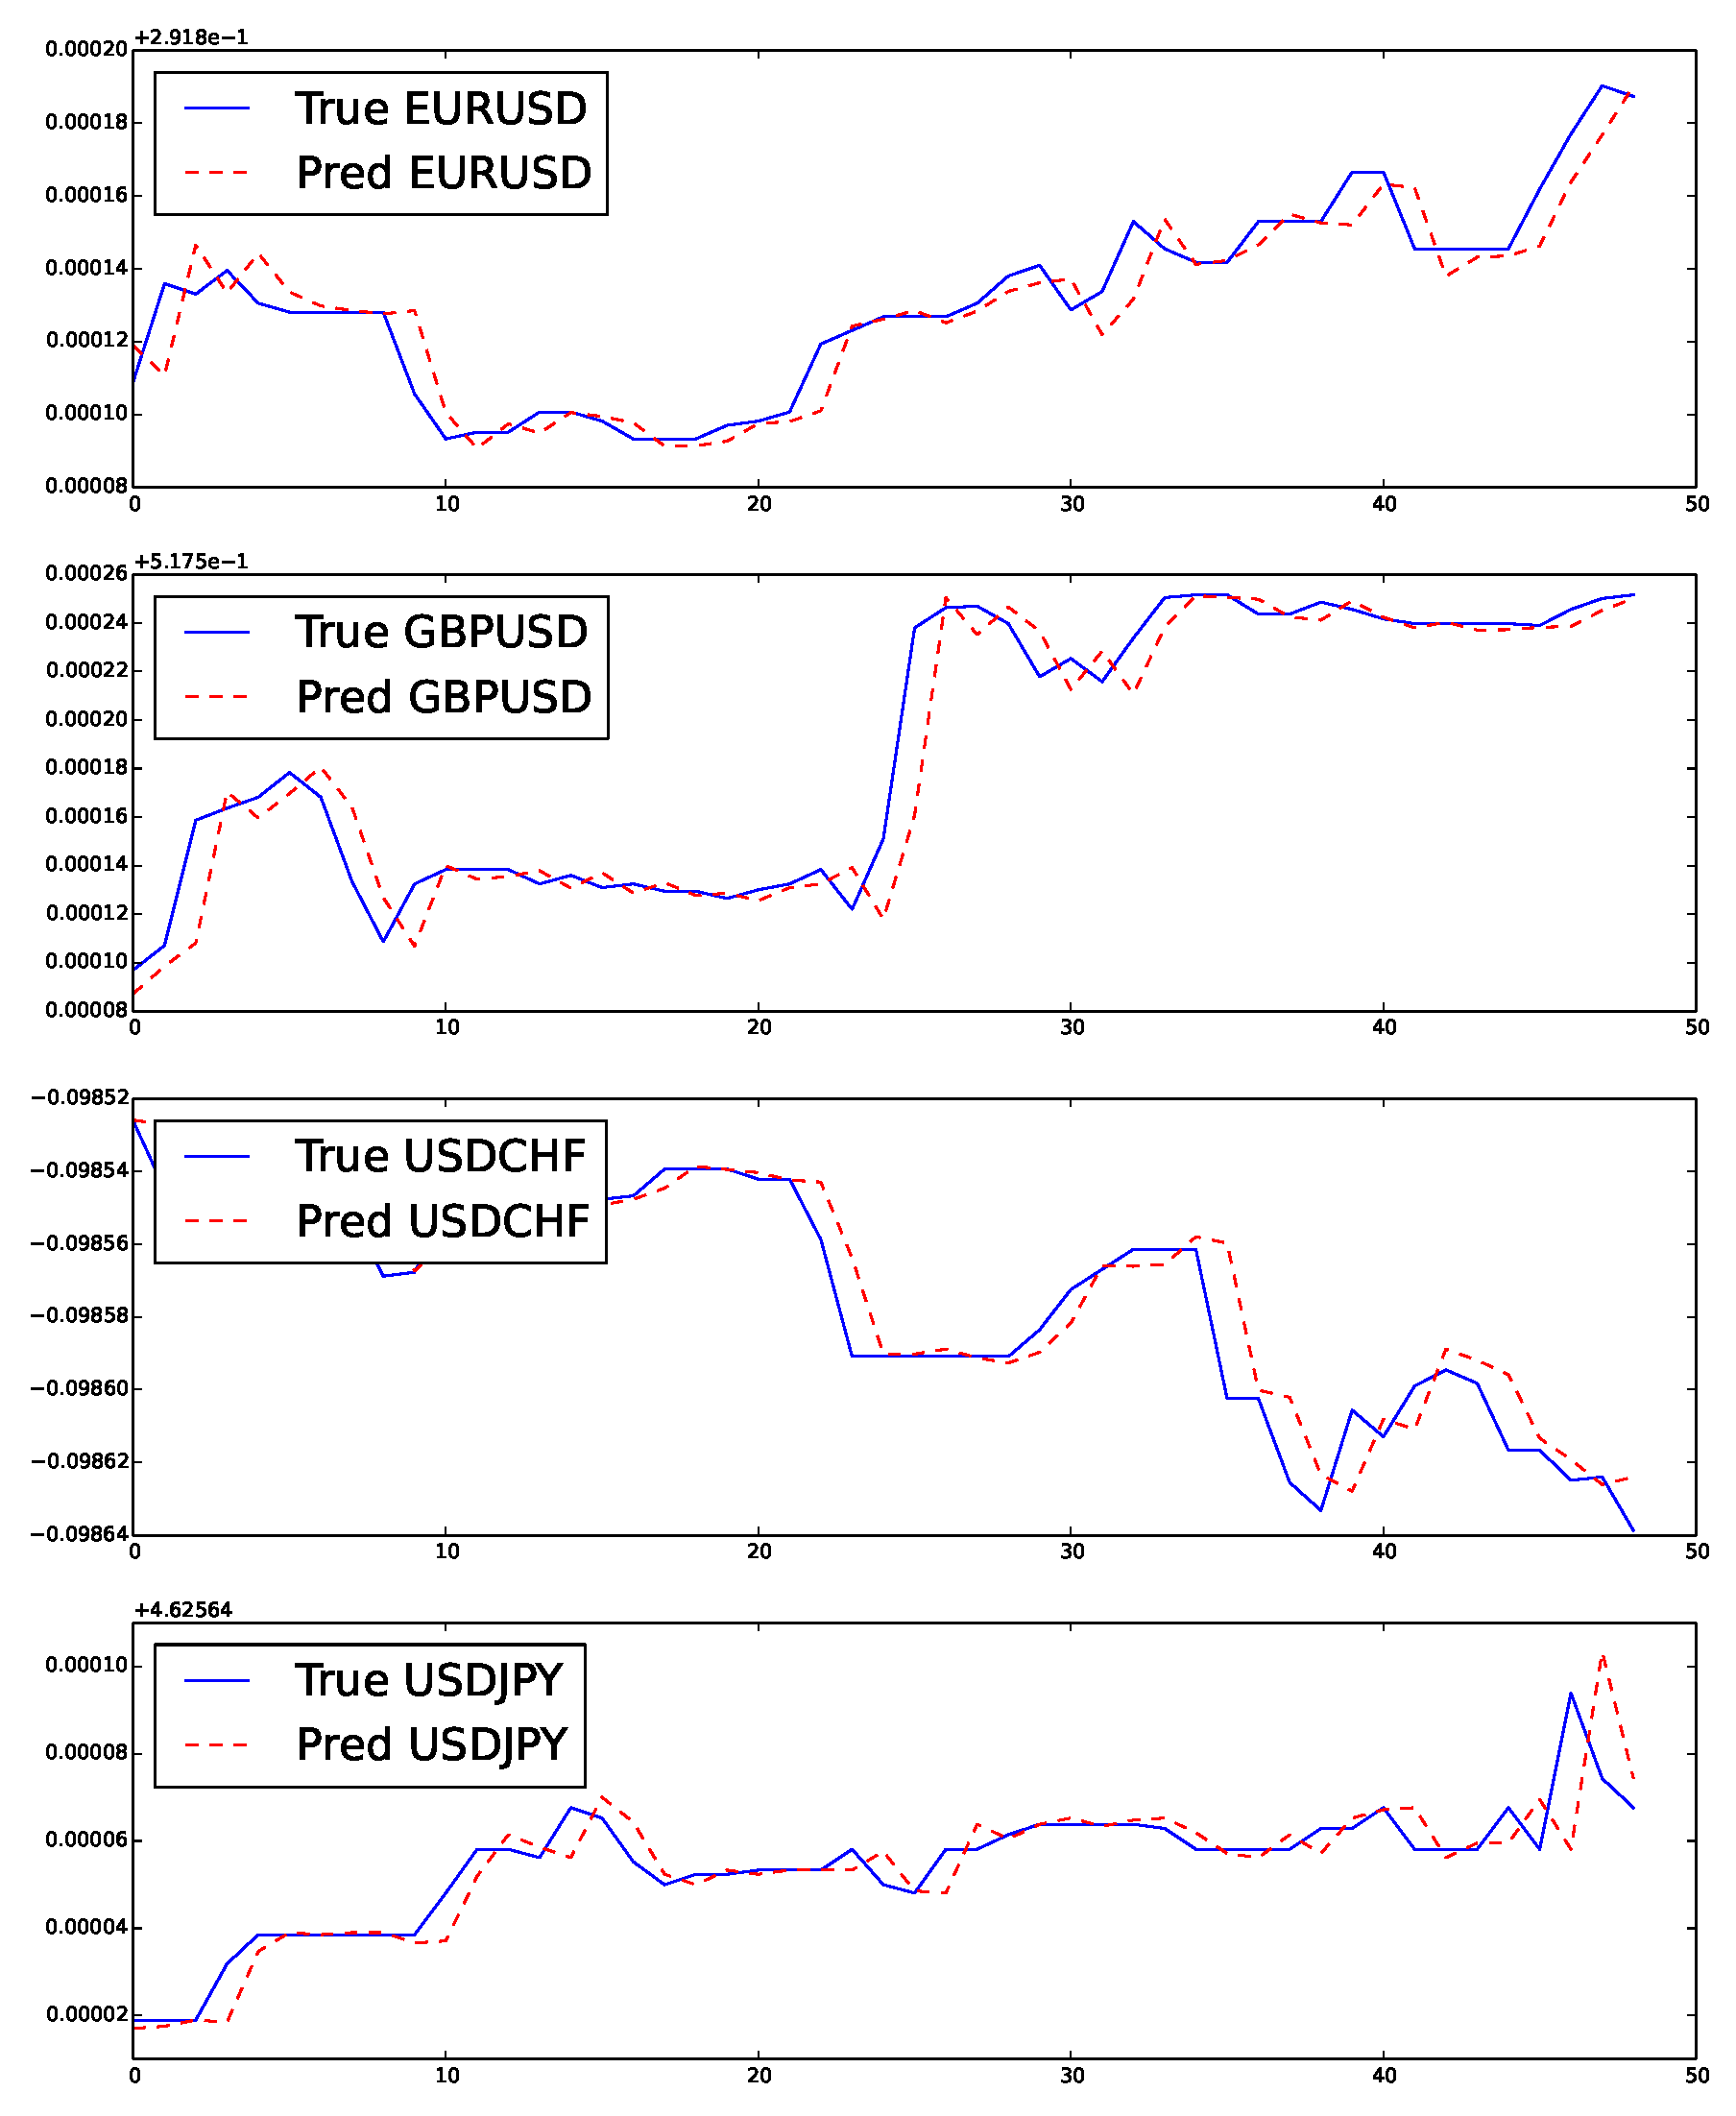
\includegraphics[width=\textwidth]{img/accuracy}
  \caption{AVECM out-of-sample forecasting for four currency rates.}
  \label{fig:accuracy}
\end{figure}


\begin{table*}[ht!]
\tiny
\caption{Performance and execution times for min MAPE criteria}
\label{tab:stats}
\begin{center}
\begin{tabular}{|l|l|l|c|c|c|c|c|}
\hline
\multicolumn{3}{|c}{Parameters} & 
\multicolumn{3}{|c}{Out-of-sample Performance} &
\multicolumn{2}{|c|}{Time[s]} \\ 
\hline

\hline
Offset & Iterations & $nparam$ & 
MAPE & MAE& RMSE& 
Sequencial & Parallel \\
\hline
 \multirow{12}{*}{19440 (London)} &
 \multirow{3}{*}{10} 
  &  12 & 1.8481E-03 & 5.1974E-04 & 7.9714E-04 & 2.64 & 2.61    \\
 &&  24 & 1.8793E-03 & 5.2935E-04 & 8.0128E-04 & 7.38 & 3.03 \\ 
 &&  47 & 1.8804E-03 & 5.2477E-04 & 7.9274E-04 & 18.86 & 3.07 \\ 
 \cline{2-8} 
 & \multirow{3}{*}{50} 
 &  12&  1.5760E-03 & 3.8559E-04 & 6.5579E-04 & 12.49 & 3.99 \\
 && 24 & 1.5645E-03 & 3.7379E-04 & 6.3128E-04 & 36.69 & 6.45 \\
 && 47 & 1.5757E-03 & 3.7336E-04 & \textbf{6.2828E-04} & 92.30 & 5.75 \\
 \cline{2-8} 
 & \multirow{3}{*}{100} 
 &  12&  1.5760E-03 & 3.8559E-04 & 6.5579E-04 & 25.00 & 5.90 \\ 
 && 24 & \textbf{1.5501E-03} & \textbf{3.6575E-04} & 6.4058E-04 & 70.58 & 9.74 \\ 
 && 47 & 1.5812E-03 & 3.8773E-04 & 6.4740E-04 & 185.05 & 11.09 \\
 \cline{2-8} 
 & \multirow{3}{*}{150} 
 &  12&  1.5760E-03 & 3.8559E-04 & 6.5579E-04 & 37.09 & 7.55 \\ 
 && 24 & 1.5501E-03 & 3.6575E-04 & 6.4058E-04 & 104.52 & 14.33 \\
 && 47 & 1.5812E-03 & 3.8773E-04 & 6.4740E-04 & 292.84 & 15.44 \\
\hline
\hline
 \multirow{12}{*}{21240 (New York)} &
 \multirow{3}{*}{10} 
  &  12 & 1.8358E-03 & 3.4906E-04 & 4.9314E-04 & 2.64 & 2.45 \\
 &&  24 & 1.8287E-03 & 3.4661E-04 & 4.9140E-04 & 7.38 & 3.03 \\
 &&  47 & 1.8402E-03 & 3.4937E-04 & 4.9298E-04 & 18.86 & 3.00 \\
 \cline{2-8} 
 & \multirow{3}{*}{50} 
 &  12&  1.6911E-03 & 3.3614E-04 & 4.8197E-04 & 12.49 & 4.00 \\
 && 24 & 1.6871E-03 & 3.3546E-04 & 4.8198E-04 & 36.69 & 6.15 \\
 && 47 & 1.6991E-03 & 3.3790E-04 & \textbf{4.8141E-04} & 92.30 & 6.17 \\
 \cline{2-8} 
 & \multirow{3}{*}{100} 
 &  12&  1.6911E-03 & 3.3614E-04 & 4.8197E-04 & 25.00 & 6.03 \\ 
 && 24 & \textbf{1.6857E-03} & \textbf{3.3510E-04} & 4.8308E-04 & 70.58 & 9.34 \\ 
 && 47 & 1.6978E-03 & 3.3766E-04 & 4.8285E-04 & 185.05 & 10.36 \\
 \cline{2-8} 
 & \multirow{3}{*}{150} 
 &  12& 1.6911E-03 & 3.3614E-04 & 4.8197E-04 & 37.09 & 7.77 \\   
 && 24 &1.6857E-03 & 3.3510E-04 & 4.8308E-04 & 104.52 & 13.84 \\
 && 47 &1.6978E-03 & 3.3766E-04 & 4.8285E-04 & 292.84 & 13.06 \\
\hline
\hline
 \multirow{12}{*}{24120 (Sidney)} &
 \multirow{3}{*}{10} 
  &  12 & 8.5847E-04 & 2.2284E-04 & 3.1202E-04 & 2.64 & 2.41 \\ 
 &&  24 & 7.9127E-04 & 1.9526E-04 & 2.9580E-04 & 7.38 & 2.86 \\ 
 &&  47 & 8.0491E-04 & 1.9578E-04 & 2.9669E-04 & 18.86 & 3.13 \\ 
 \cline{2-8} 
 & \multirow{3}{*}{50} 
 &  12& 9.1471E-04 & 2.2555E-04 & 3.1371E-04 & 12.49 & 4.02 \\ 
 && 24 &7.3172E-04 & 1.8017E-04 & 2.8054E-04 & 36.69 & 5.45 \\
 && 47 &7.3172E-04 & 1.8017E-04 & 2.8054E-04 & 92.30 & 6.48 \\
 \cline{2-8} 
 & \multirow{3}{*}{100} 
 &  12& 8.0458E-04 & 2.0706E-04 & 2.9542E-04 & 25.00 & 5.90 \\ 
 && 24 &\textbf{6.2547E-04} & 1.6451E-04 & 2.5945E-04 & 70.58 & 9.23 \\ 
 && 47 &6.3424E-04 & \textbf{1.6400E-04} & \textbf{2.5849E-04} & 185.05 & 11.13 \\
 \cline{2-8} 
 & \multirow{3}{*}{150} 
 &  12&  7.2437E-04 & 1.8782E-04 & 2.8016E-04 & 37.09 & 7.83 \\ 
 && 24 & 6.2547E-04 & 1.6451E-04 & 2.5945E-04 & 104.52 & 12.42 \\
 && 47 & 6.2547E-04 & 1.6451E-04 & 2.5945E-04 & 292.84 & 13.95 \\
\hline
\hline
 \multirow{12}{*}{24840 (Tokyo)} &
 \multirow{3}{*}{10} 
  &  12 & 1.0787E-03 & 3.3948E-04 & 5.5145E-04 & 2.64 & 2.45 \\ 
 &&  24 & 1.0823E-03 & 3.3992E-04 & 5.4697E-04 & 7.38 & 2.96 \\ 
 &&  47 & 1.0885E-03 & 3.4462E-04 & 5.5231E-04 & 18.86 & 3.05 \\
 \cline{2-8} 
 & \multirow{3}{*}{50} 
 &  12& 1.0753E-03 & 3.4955E-04 & 5.7100E-04 & 12.49 & 3.97 \\ 
 && 24 &1.1042E-03 & 3.5395E-04 & 5.6747E-04 & 36.69 & 6.08 \\ 
 && 47 &1.1238E-03 & 3.5794E-04 & 5.7330E-04 & 92.30 & 6.67 \\ 
 \cline{2-8} 
 & \multirow{3}{*}{100} 
 &  12& \textbf{8.4691E-04} & \textbf{2.8979E-04} & \textbf{5.2553E-04} & 25.00 & 5.74 \\ 
 && 24 &8.6649E-04 & 2.9405E-04 & 5.2874E-04 & 70.58 & 10.29 \\
 && 47 &8.8877E-04 & 2.9821E-04 & 5.3796E-04 & 185.05 & 9.00 \\
 \cline{2-8} 
 & \multirow{3}{*}{150} 
 &  12& 8.5021E-04 & 2.9579E-04 & 5.2707E-04 & 37.09 & 7.54 \\ 
 && 24 &8.6350E-04 & 2.9183E-04 & 5.2837E-04 & 104.52 & 13.05 \\
 && 47 &8.8597E-04 & 2.9594E-04 & 5.3759E-04 & 292.84 & 13.82 \\
\hline
\end{tabular}
\end{center}
\end{table*}





\subsection{Execution times} \label{sec:exectimes}
We ran AVECM 100 ($outit$ in algorithm~\ref{alg:AVECM}) iterations.
Table~\ref{tab:stats} shows execution times and performance measures for
different times of the market, in-sample iterations and number of parameters used.
The number of parameters represents the possible combinations of values for $L$ and
$P$. The $L$ parameter was always chosen between 100 and 4000 and $nparams$
determines how many values in this range were considered. $p$ always took values
between 1 and 5. Execution times were measured using the Time python library.

Execution time depends directly on $L$ and $p$ since they determine the size of
matrix $\mathbf{A}$ and therefore affects the OLS function execution time.
Therefore, if we try more combinations of $L$ and $p$ (increasing $nparam$) the
algorithm will take longer. However, the idea is to improve accuracy measures
ensuring execution times below 10 seconds (the time series frequency). 

Table ~\ref{tab:stats} shows that best performance accuracy measures are
achieved in times near or below 10 seconds in the parallel version. Contrarily,
sequential times are high, above 10 seconds in most of the cases.

Despite there being some parallel execution times above 10 seconds, the
performance measures didn't improve and so they can be dismissed.

Figure~\ref{fig:extimes} shows sequential and parallel time and speed-up
computing time for VECM with 100 iterations.

\begin{figure}[!h]
  \centering
  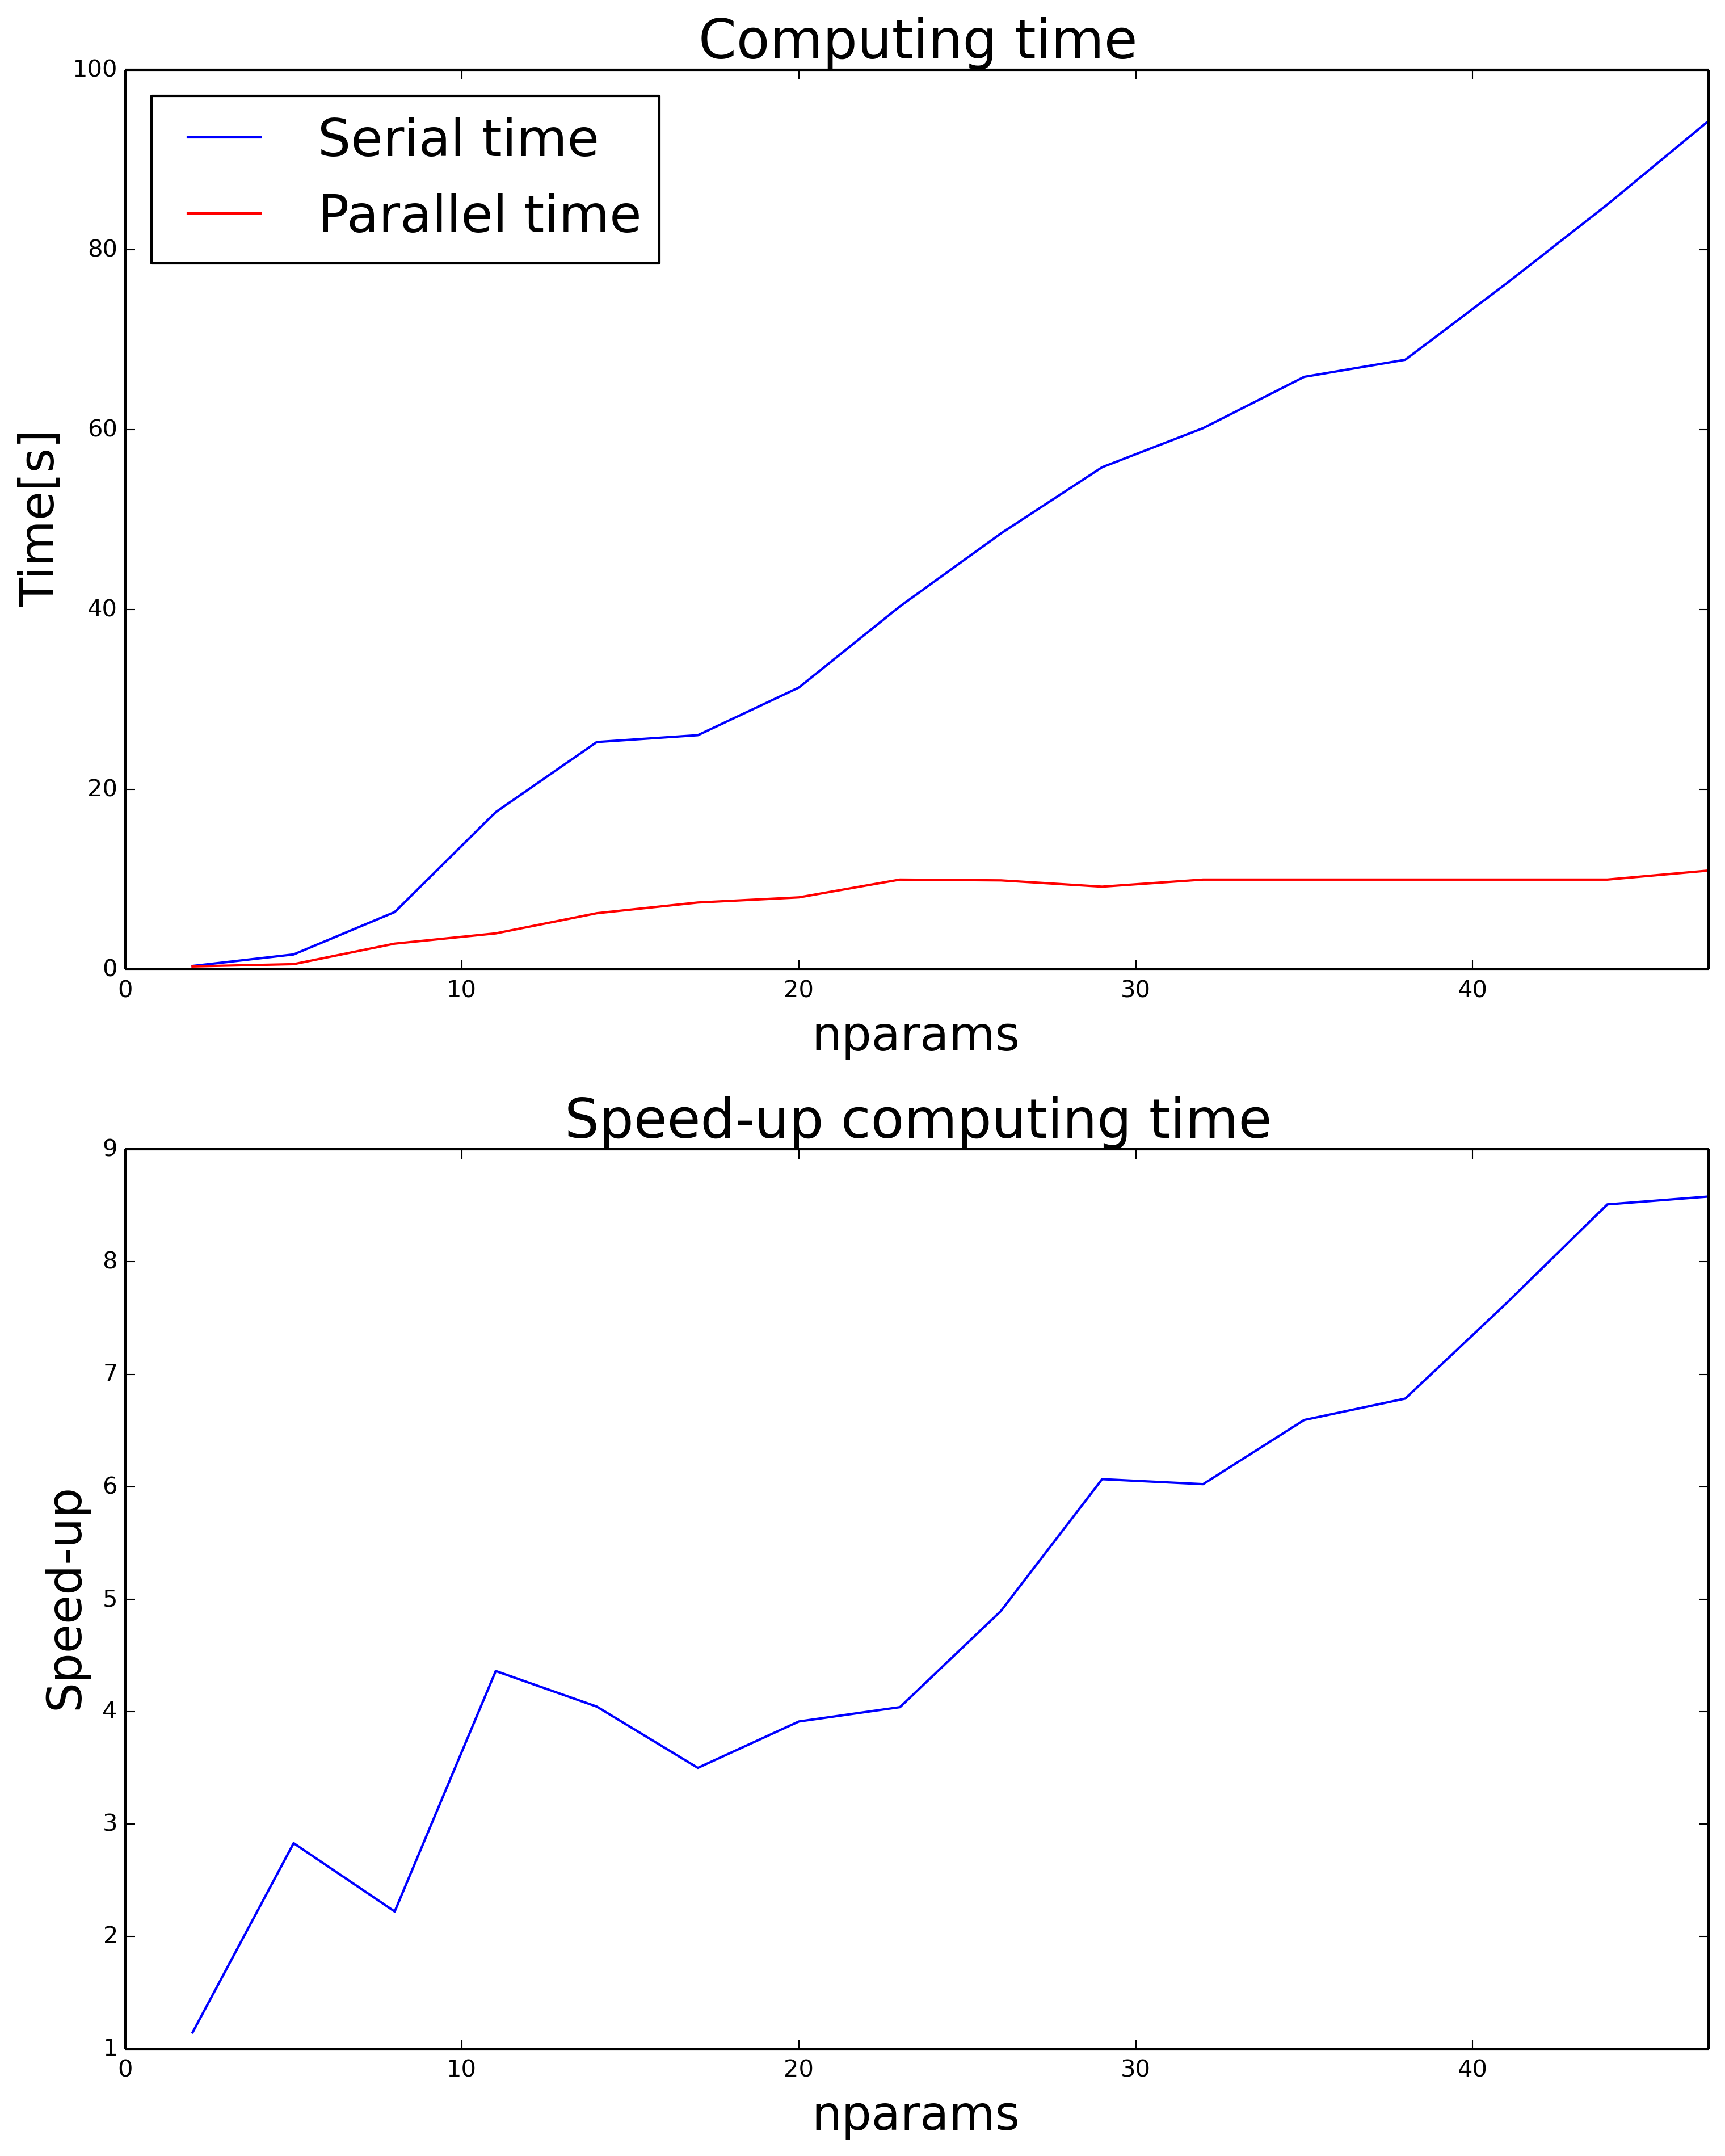
\includegraphics[width=0.7\textwidth]{img/extimes}
  \caption{Computing time of sequential and parallel algorithm is shown in the
  upper figure. Speed-up is shown below.}
  \label{fig:extimes}
\end{figure}


Execution times do not consider the loading data time, just the finding of
best parameters and the building the VECM model. The time MPI spends
transferring data and synchronising process is about two seconds independently
of the number of process considered.

\section{Conclusions}
\label{sec:conclusions}
Cointegration in financial time series has been largely studied and the 
Johansen method is commonly used to obtain it. 
In practice it has been found that cointegration relations change with time. 
However, cointegration model-based such as VECM assumes that cointegration
remains unchanged in time. 
We empirically showed that the Johansen method is sensitive to the number
of lags but also to the amount of data considered.

Moreover, we introduced the notion of {\em percentage of cointegration\/} and
have found that out-of-sample forecast performance is related to the value of
this figure in the last samples.  We used this information to set the model
parameters.  Our proposal AVECM consists then on an adaptive algorithm to update VECM
parameters every time that new data is available. These parameters are found by
maximising the percentage of cointegration of the last samples or iterations.

Determining VECM parameters was the most expensive routine and it was run
using parallel processes using MPI which allowed a grid search within a range of
values for $L$ and $p$ to be made.
Tests were done using real currency rates data. 
Our proposal was tested in several scenarios using different times of
the day to show its behaviour related to the opening times of
financial markets.

Results showed that our proposed AVECM improves performance measures by finding
parameters of $L$ and $p$ maximising the percentage of cointegration.
These facts were consistent for different times of the day. 
We found that increasing the number of parameters will always lead to
better performance measures. Furthermore, in the case of Tokyo 
financial market opening time, MAPE reduced an order from $10^{-3}$ to $10^{-4}$.

The parallel implementation allowed the execution times to be reduced
more than ten times and therefore a response time was obtain before 10
seconds. Since we used 10-second frequency we can say that our proposal is suitable
for use in an online context for real applications because response times
were less than this frequency.

For future study, it would be interesting to explore the relation between
cointegration and performance in order to propose new criteria for
improving VECM parameters.



\chapter{Intraday Forex rates forecasting using an online cointegration approach}

High frequency forex rates 
Vector error correction model (VECM) parameters are commonly obtained using the
ordinary least squares method. Since this parameters could be sensitive to the
data, this proposal is to get these parameters using ridge regression which
could lead to a better generalization capability. In order to give with a
real-time response, an online version of VECM (OVECM) is proposed. OVECM solves
VECM considering only a sliding window of historical data and therefore
better response times could be achieved.


\section{The problem}

VECM introduces the long-run relationship among a set of cointegrated variables
as an error correction term. VECM is a special case of the vector autorregresive
model (VAR) model. VAR model expresses future values as a linear combination of
variables past values.  However, VAR model cannot be used with non-stationary
variables, which is a common feature of financial assets. VECM is a linear model
but in terms of variable differences. If cointegration exists, variable
differences are stationary and they introduce an error correction term which
adjusts coefficients to bring the variables back to equilibrium. In finance,
many economic time series turn to be stationary when they are differentiated and
cointegration restrictions often improves forecasting~\cite{duy1998}. Therefore,
VECM has been widely adopted.

Both VECM and VAR model parameters are obtained using ordinary least squares
(OLS) method. OLS has two main problems: is sensitive to errors on input data
and involves many calculations. The former problem is commonly solved using
Ridge Regression (RR) \cite{hoerl1970} which introduces a regularization
parameter that leads to an unbiased estimation with better generalization
capability. The second problem of computational complexity depends on the number
of past values and observations considered.  Recently, online learning
algorithms have been proposed to solve problems with large data sets because of
their simplicity and their ability to update the model when new data is
available. 

Our proposal is an online formulation of the VECM called Online VECM (OVECM)
based on consideration of only a sliding window of the historical data.  OVECM
introduces matrix optimizations in order to reduce the number of operations and
also takes into account the fact that cointegration vector space doesn't
experience large changes with small changes in the input data. Moreover, OVECM
uses RR instead of OLS to obtain VECM parameters. Our method is later tested using four
currency rates from the foreign exchange market with a frequency of 10 seconds.
Model efectiveness is focused on out-of-sample forecast rather than in-sample
fitting.  This criteria allows the OVECM prediction capability to be expressed
rather than just explaining data history. Our method performance is compared
with its optimal offline algorithm.


%The next sections are organized as follows: section~\ref{sec:background}
%presents the VAR and VECM, the OVECM algorithm proposed is presented in
%section~\ref{sec:methodology}. Section~\ref{sec:results} gives a description of
%the data used and the tests carried on to show accuracy and time comparison of
%our proposal against the traditional VECM and
%section~\ref{sec:conclusions} includes conclusions and a proposal for future
%tudy.


\section{Methodology}

Since financial problems are stream data problems, it is unfeasible to include
all input data in a VECM model. Our proposal consists on an online version of
VECM (OVECM) capable of updating the model with new arrival data and give
responses in a short period of time. OVECM only considers a time varying window
of historical data and the using of RR or its variant AAR (Aggregating Algorithm
for Regression) as an alternative of OLS to get model parameters.

On the other hand, getting cointegration vectors using Johansen method is also
an expensive procedure. However, since cointegration
vectors represent the long-run relationship between the time series, they
vary little in time. Our proposal obtains new cointegration vectors only when
this long-term relationship changes. This change is detected by tracking 
the Mean Absolute Percentage Error (MAPE) of the last $n$ in-sample forecasts.

%Since VECM is a model based on time series differences, the MAPE is obtained
%from $\Delta \mathbf{y}$ as following:
% 
%\begin{equation}\label{eq:MAPE}
%\text{MAPE}[t] = \frac{1}{n} \sum_{i=1}^{n} \left| 
%\frac{\Delta \mathbf{y}_{\text{true}}[t-i]-\Delta
%\mathbf{y}_{\text{pred}}[t-i]}{\Delta \mathbf{y}_{\text{true}[t-i]}}
%\right| \, , 
%\end{equation}
%
%\noindent where $\Delta \mathbf{y}_{\text{true}}$ is the actual value of the
%time series $\mathbf{y}$ differences and $\Delta \mathbf{y}_{\text{pred}}$ is
%their forecast value.




%The method proposed consists of
%a modification of RR considering a sliding window which contains only
%the last $L$ samples %and the new input $\mathbf{x}_t$, 
%i.e. $\{\mathbf{x}_i\}_{i=t-L+1}^{t-1}$. 

VECM($p$) for $l$ cointegrated variables has the following form:

\begin{equation}\label{eq:vecfull}
\Delta\mathbf{y}_t 
= \boldsymbol{\alpha\beta}^\top\mathbf{y}_{t-1} 
  + \sum_{i=1}^{p-1}\boldsymbol{\Phi}_i^*\,\Delta\mathbf{y}_{t-i}
  + \mathbf{c} + \boldsymbol{\epsilon}_t \qquad \forall t = p+1,\dots,N.
\end{equation}

Transposing each equation of the system (\ref{eq:vecfull}) we can write
the VECM($p$) model in block-matrix form as:
\begin{equation}\label{eq:vareq}
\mathbf{B} = 
\mathbf{A} \mathbf{X} + 
\mathbf{E} \, , 
\end{equation}
%
\noindent where $\mathbf{B}$ dimension is $((N-p)\times l)$, $\mathbf{A}$
dimension is $((N-p)\times(r+(p-1)l +1))$, $\mathbf{X}$ dimension is $((r+(p-1)l
+1)\times l)$, $\mathbf{E}$ dimension is $((N-p)\times l)$ and $r$ is the number
of cointegration vectors:
%
\begin{alignat}{3}
\mathbf{B}
&= \begin{bmatrix}
   \Delta\mathbf{y}_{p+1}^\top \\
   \Delta\mathbf{y}_{p+2}^\top \\
   \vdots \\
   \Delta\mathbf{y}_N^\top
   \end{bmatrix}
&\quad
\mathbf{X}
&= \begin{bmatrix}
   \boldsymbol{\alpha}^\top \\
   \boldsymbol{\Phi}_1^{*\top} \\
   \boldsymbol{\Phi}_2^{*\top} \\
   \vdots \\
   \boldsymbol{\Phi}_{p-1}^{*\top} \\
   \mathbf{c}^\top
   \end{bmatrix}
&\quad
\mathbf{E}
&= \begin{bmatrix}
   \boldsymbol{\epsilon}_{p+1}^\top \\
   \boldsymbol{\epsilon}_{p+2}^\top \\
   \vdots \\
   \boldsymbol{\epsilon}_N^\top \\
   \end{bmatrix}
\end{alignat}
\noindent and 
\begin{align}
\mathbf{A} 
&= \begin{pmat}[{....|}]
   \mathbf{y}_p^\top \boldsymbol{\beta} & \Delta \mathbf{y}_p^\top & \Delta\mathbf{y}_{p-1}^\top & \dots 
                    & \Delta\mathbf{y}_2^\top & 1 \cr
   \mathbf{y}_{p+1}^\top  \boldsymbol{\beta} &\Delta\mathbf{y}_{p+1}^\top & \Delta\mathbf{y}_p^\top & \dots
                       & \Delta\mathbf{y}_3^\top & 1 \cr
   \vdots & \vdots & \vdots & \ddots & \vdots & \vdots \cr
   \mathbf{y}_{N-1}^\top  \boldsymbol{\beta} &\Delta\mathbf{y}_{N-1}^\top & \Delta\mathbf{y}_{N-2}^\top & \dots 
                       & \Delta\mathbf{y}_{N-p-1}^\top & 1 \cr
   \end{pmat}\, .
\end{align}
%Taking into account the error term $\mathbf{E}$, equation~(\ref{eq:vareq}) 
%can be solved with respect to $\mathbf{X}$ using the ordinary least
%squares estimation.
However, the number of rows of matrix $\mathbf{A}$ increases with the number of
observations $\mathbf{y}_t$. Our proposal considers only the most recent $L$
rows of matrices $\mathbf{A}$ and $\mathbf{B}$ defined as  $\mathbf{A}(t)$ and
$\mathbf{B}(t)$:

\begin{equation}
\label{eq:notation}
	\mathbf{A}(t) = 
\left[
  \begin{tabular}{c>{$}c<{$}c}
    --- & \mathbf{a}^{\top}_{t-L} & ---\\
    --- & \mathbf{a}^{\top}_{t-L+1} & ---\\
    & \vdots & \\
    --- & \mathbf{a}^{\top}_{t} & ---
  \end{tabular}
\right]
\quad \text{and} \quad
\mathbf{B}(t) =
\left[
  \begin{tabular}{c>{$}c<{$}c}
    --- & \mathbf{b}_{t-L} & ---\\
    --- & \mathbf{b}_{t-L+1} & ---\\
    & \vdots & \\
    --- & \mathbf{b}_{t} & ---
  \end{tabular}
\right] \, ,
\
\end{equation}

\noindent so that VECM parameters $\mathbf{X}(t)$ are found using the following
equation:

\begin{equation}
\mathbf{B}(t) = \mathbf{A}(t) \mathbf{X}(t) + \mathbf{E}(t)\\
\end{equation}

The RR solution $\mathbf{\hat{X}}(t)$ using the sliding window matrices defined above
is:

\begin{equation}
\label{eq:oproblem}
\mathbf{\hat{X}}(t)=\mathbf{S}(t)^{-1} \mathbf{W}(t) \, ,
\end{equation}

\noindent where $\mathbf{S}{t}$ and $\mathbf{W}{t}$ are define as:

\begin{eqnarray*}
\mathbf{S}(t) =&{\bf A}(t)^\top{\bf A}(t)+ \lambda \mathbb{I} &=
\sum_{i=0}^L \mathbf{a}_{t-i}\mathbf{a}_{t-i}^\top + \lambda \mathbb{I}
\label{eq:S} \\
\mathbf{W}(t) =& {\bf A}(t)^\top{\bf B}(t) &= 
\sum_{i=0}^L \mathbf{a}_{t-i}\mathbf{b}_{t-i} 
\label{eq:W}
\end{eqnarray*}

It is worth noticing that, at the next time step, the matrices $\mathbf{S}(t+1)$
and $\mathbf{W}(t+1)$ are slightly different to $\mathbf{S}(t)$ and
$\mathbf{W}(t)$:

\begin{eqnarray*}
\mathbf{S}(t+1)&=&
\mathbf{S}(t) +
\mathbf{a}_{t+1}
\mathbf{a}_{t+1}^\top -
\mathbf{a}_{t-L} \mathbf{a}_{t-L}^\top \\
\mathbf{W}(t+1)&=&
\mathbf{W}(t) +
\mathbf{a}_{t+1}
\mathbf{b}_{t+1} -
\mathbf{a}_{t-L} \mathbf{b}_{t-L} \, .
\end{eqnarray*}

%Agregar solo si se decide agregar Sherman-Morrison
%Therefore the Sherman-Morrison-Woodbury formula can be used to reduce inverse matrix
%calculations.

The algorithm~\ref{alg:proposal} shows OVECM using three different
methods for geting model parameters: OLS, RR, AAR which leads to three different
algorithms OVECM-OLS, OVECM-RR, OVECM-AAR:

\begin{algorithm}[ht]
\begin{algorithmic}[1]
\REQUIRE $\,$ \\
$\mathbf{y}$: matrix with $N$ input vectors and $l$ time series\\
$p$: number of past values \\
method: \{'OLS','RR','AAR'\} \\
$\lambda$: regularization parameter (only requires for RR and AAR methods) \\
$L$: window size of data($L<N$) \\
$\text{mean\_error}$: MAPE threshold \\
$n$: windows size to obtain in-sample MAPE \\
\ENSURE  $\,$ \\
$\{\mathbf{y}_{\text{pred}}[L+1],\dots, \mathbf{y}_{\text{pred}}[N]\}$: model predictions 
\STATE solver = new \texttt{Solver}(method,$\lambda$) \\
\FOR { $t =1$ to $N-L$ }
    \STATE $\mathbf{Y} \gets \mathbf{y}[t:t+L-1]$
    \STATE $\mathbf{y}_t \gets \mathbf{y}[t+L]$
	\IF {$t = 1$}
	    \STATE{$v \gets \texttt{getJohansen}(\mathbf{Y},p)$}
	    \STATE{$[\mathbf{A} \quad \mathbf{B}] \gets
        \texttt{vecMatrix}(\mathbf{Y},p,v)$}
        \STATE \texttt{solver.init\_model($\mathbf{A},\mathbf{B}$)} 
    \ENDIF
	\STATE{[$\mathbf{A} \quad \mathbf{B} \quad \mathbf{a}_t \quad \mathbf{a}_L \quad \mathbf{b}_t \quad
    \mathbf{b}_L ] \gets
    \texttt{vecMatrixOnline}(\mathbf{Y},\mathbf{y}_t,p,v)$}
    \STATE $[\mathbf{X} \quad \mathbf{y}_{\text{pred}}[t]] \gets \texttt{solver.regression}
    (\mathbf{A},\mathbf{B},\mathbf{a}_t,\mathbf{b}_t)$
    \STATE $\mathbf{Y}_{\text{pred}} = \mathbf{AX}[-n:]+\mathbf{Y}[-n-1:-1]$
    \STATE $\mathbf{e} = \texttt{mape}(\mathbf{Y}_{\text{pred}},\mathbf{Y}[-n:])$
    \IF {$\texttt{mean}(\mathbf{e}) > \text{mean\_error}$}
	    \STATE{$v \gets \texttt{getJohansen}(\mathbf{Y},p)$}
	    \STATE{$\mathbf{A} \gets
        \texttt{vecMatrixUpdate}(\mathbf{A},\mathbf{Y},p,v)$}
        \STATE \texttt{solver.init\_model($\mathbf{A},\mathbf{B}$)} 
	    \STATE{$[\mathbf{a}_t \quad \mathbf{b}_t] \gets
        \texttt{vecMatrixOnline}(\mathbf{Y},\mathbf{y}_t,p,v)$}
        \STATE $[\mathbf{X} \quad \mathbf{y}_{\text{pred}}[t]] \gets \texttt{solver.regression}
        (\mathbf{A},\mathbf{B},\mathbf{a}_t,\mathbf{b}_t)$
    \ENDIF
\STATE{$[\mathbf{A} \quad \mathbf{B}] \gets
\texttt{matrixUpdate}(\mathbf{A},\mathbf{B},\mathbf{a}_t,\mathbf{b}t)$}
\ENDFOR
\end{algorithmic}
\caption{OVECM: Online VECM}
\label{alg:proposal}
\end{algorithm}


Our proposal considers the following:

\begin{itemize}
\item The function \texttt{getJohansen} returns cointegration vectors given by the
Johansen method considering the trace statistic test at 95\% level of
significance. This procedure is called at the first step of the algorithm and
every time in-sample MAPE ($\mathbf{e}$) exceeds threshold error defined (mean\_error).
\item The function \texttt{vecMatrix} returns VECM
matrices $\mathbf{A}(t),\mathbf{B}(t)$ shown in equation~(\ref{eq:notation}). This
method is only required at the first step.
\item The function \texttt{vecMatrixOnline} returns new rows $\mathbf{a}_t^\top$ and
$\mathbf{b}_t^\top$ given new input data $\mathbf{y}_t$.
\item The Solver class (see algorithm \ref{alg:solver}) obtain VECM parameters  
using RR, AAR or OLS methods.
\item The function \texttt{vecMatrixUpdate} updates matrix $\mathbf{A}$ when new
cointegration vectors are required (matrix $\mathbf{B}$ is not affected). Model
parameters $\mathbf{X}$ is also updated later.
%\item The number of cointegration vectors is set as a parameter (aun no lo
%coloco en el algoritmo).
%\item In order to set VECM parameter: $L$ and $p$, we use the Akaike Information
%Criterion (AIC). RR parameter $\lambda$ was done by cross-validation.
%\item Obtain VECM parameter $\mathbf{X}(t)$ in equation \ref{eq:optsolSLAAR} requires
%to calculate the inverse of matrix $\mathbf{S}(t+1)$ which is an expensive
%routine.However, since we already know $\mathbf{S}(t)^{-1}$ we can use
%Sherman-Morrison-Woodbury twice~\ref{eq:SMW}.
\end{itemize}




\begin{algorithm}[ht]
\begin{algorithmic}[1]
\REQUIRE $\,$ \\
method: \{'OLS','RR','AAR'\} \\
$\mathbf{A}$: VECM design matrix \\
$\mathbf{B}$: VECM dependant variables \\
$\mathbf{a}_t$: new row of $\mathbf{A}$ \\
$\mathbf{b}_t$: new row of $\mathbf{B}$ \\
$\gamma$: regularization parameter \\
$n$: windows size to obtain in-sample MAPE \\
\ENSURE  $\,$ \\
$\mathbf{X}$: regression solution \\
$\mathbf{e}$: in-sample MAPE \\
%\quad \\
%\texttt{init}($L,\lambda$)
%\STATE self.L = L
%\STATE self.lambda = $\lambda$
\quad \\
\texttt{init\_model}($\mathbf{A},\mathbf{B}$)
\STATE $ [m \quad n] = \text{size}(\mathbf{A}) $ 
\STATE $\mathbf{S} = \displaystyle \sum_{i=1}^m \mathbf{a}_i \mathbf{a}_i^\top + \gamma \mathbb{I}$
\STATE $\mathbf{W} = \displaystyle \sum_{i=1}^m \mathbf{a}_i \mathbf{b}_i$
\quad \\
\texttt{regression}($\mathbf{A},\mathbf{B},\mathbf{a_t},\mathbf{b_t}$) \\
\IF {method == 'OLS'}
        \STATE $\mathbf{X}=(\mathbf{A}^\top \mathbf{A})^{-1}\mathbf{A}^\top
        \mathbf{B}$
\ELSIF {method == 'RR'}
        \STATE $\mathbf{X} = \mathbf{S}^{-1} \mathbf{W} $
        \STATE $\mathbf{S} = \mathbf{S}+
        \mathbf{a}_t \mathbf{a}_t^\top-
        \mathbf{a}_1 \mathbf{a}_1^\top$
        \STATE $\mathbf{W} = \mathbf{W} + \mathbf{a}_t \mathbf{b}_t$
\ELSIF {method == 'ARR'}
        \STATE $\mathbf{S} = \mathbf{S}+
        \mathbf{a}_t \mathbf{a}_t^\top-
        \mathbf{a}_1 \mathbf{a}_1^\top$
        \STATE $\mathbf{X} = \mathbf{S}^{-1} \mathbf{W} $
        \STATE $\mathbf{W} = \mathbf{W} + \mathbf{a}_t \mathbf{b}_t$
\ENDIF
\STATE $\mathbf{y}_{\text{pred}} = \mathbf{X}^\top \mathbf{a}_t$
\end{algorithmic}
\caption{Solver Class for Regression Methods}
\label{alg:solver}
\end{algorithm}




% Aqui se puede hablar de evaluation using competitive analysis. The idea
%of competitiveness is to compare the output generated by an online algorithm to
%the output produced by an optimal offline algorithm. An optimal online algorithm
%is an omniscient algorithm that knows the entire input data in advance and can
%compute an optimal output. The better an online algorithm approximates the
%optimal solution, the more competitive this algorithm is.


The proposal was compared against an optimal online algorithm which is a time varying
VECM (OOVECM). Algorithm ~\ref{alg:OOVECM} shows this modification:


\begin{algorithm}[ht]
\begin{algorithmic}[1]
\REQUIRE $\,$ \\
$\mathbf{y}$: matrix with $N$ input vectors and $l$ time series\\
$p$: number of past values \\
$L$: sliding window size ($L<N$) \\
\ENSURE  $\,$ \\
$\{\Delta \mathbf{y}_{\text{pred}}[L+1],\dots,\Delta \mathbf{y}_{\text{pred}}[N]\}$: model predictions 
\FOR { $i =0$ to $N-L$ }
    \STATE $\mathbf{y}_i \gets \mathbf{y}[i:i+L]$
	\STATE{$v \gets \texttt{getJohansen}(\mathbf{y}_i,p)$}
	\STATE{$[\mathbf{A} \quad \mathbf{B}] \gets
    \texttt{vecMatrix}(\mathbf{y}_i,p,v)$}
    \STATE $\mathbf{X} \gets \text{OLS} (\mathbf{A},\mathbf{B})$%\mathbf{(A^\top A)^{-1}A^\top B}$
    \STATE $\Delta \mathbf{Y}_{\text{true}}[i] \gets \mathbf{B}[-1,:]$
    \STATE $\Delta \mathbf{Y}_{\text{pred}}[i] \gets \mathbf{A}[-1,:] \times \mathbf{X}$
\ENDFOR
    \STATE $\text{MAPE} \gets \texttt{mape}(\Delta \mathbf{Y}_{\text{true}}, \Delta
    \mathbf{Y}_{\text{pred}})$
\end{algorithmic}
\caption{OOVECM: Optimal Online Vector Error Correction Model}
\label{alg:OOVECM}
\end{algorithm}


%%Solo para tesis
%\section{Online VEC model}
%
%If we want to update the VEC model with new input data
%$\mathbf{y}_{T+1}$, we have to add a new row in matrices
%$\mathbf{Y,X}$ and $\mathbf{E}$. 
%
%\begin{eqnarray}
%\mathbf{Y} &=& 
%                \left[ \begin{array}{ccc}
%               \quad & \mathbf{\Delta y}_{p+1} & \quad \\ \hline
%               \quad & \mathbf{\Delta y}_{p+2} & \quad \\ \hline
%               \quad & \vdots & \quad \\ \hline 
%               \quad & \mathbf{\Delta y}_T & \quad \\ 
%               \quad & \color{red}\mathbf{\Delta y}_{T+1} & \quad 
%               \end{array} \right]
%             \\
%\mathbf{\Phi^*} &=& 
%                \left[ \begin{array}{ccc}
%               \phi_{p-1}^* \\ 
%               \vdots \\ 
%               \phi_{1}^* \\
%               \alpha \\
%                c   
%               \end{array} \right]
%\\
%\mathbf{X} &=& \begin{bmatrix} \label{offX}
%   \mathbf{\Delta y}_2 & \dots & \mathbf{\Delta y}_{p-1} &
%   \mathbf{\Delta y}_{p} & \beta'\mathbf{y}_{p} & 1\\
%   \mathbf{\Delta y}_3 & \dots & \mathbf{\Delta y}_{p} &
%   \mathbf{\Delta y}_{p+1} & \beta'\mathbf{y}_{p+1} &1\\
%   \vdots &  \ddots & \vdots & \vdots & \vdots & \vdots\\
%   \mathbf{\Delta y}_{T-p+1} & \dots & \mathbf{\Delta y}_{T-2} &
%   \mathbf{\Delta y}_{T-1} & \beta'\mathbf{y}_{T-1} &1 \\
%   \color{red} \mathbf{\Delta y}_{T-p+2} & \dots & \color{red}\mathbf{\Delta y}_{T-1} &
%   \color{red}\mathbf{\Delta y}_{T} & \color{red}\beta'\mathbf{y}_{T}
%   & \color{red} 1
%   \end{bmatrix}
%\\
%\mathbf{E} &=& \begin{bmatrix}
%              \mathbf{\epsilon}_{p+1} \\ \vdots \\ \mathbf{\epsilon}_T
%              \\ \color{red}\mathbf{\epsilon}_{T+1}
%             \end{bmatrix}
%\end{eqnarray}



\section{Experiments}

\begin{figure}[!h]
  %\vspace{-0.8cm}
  \centering
  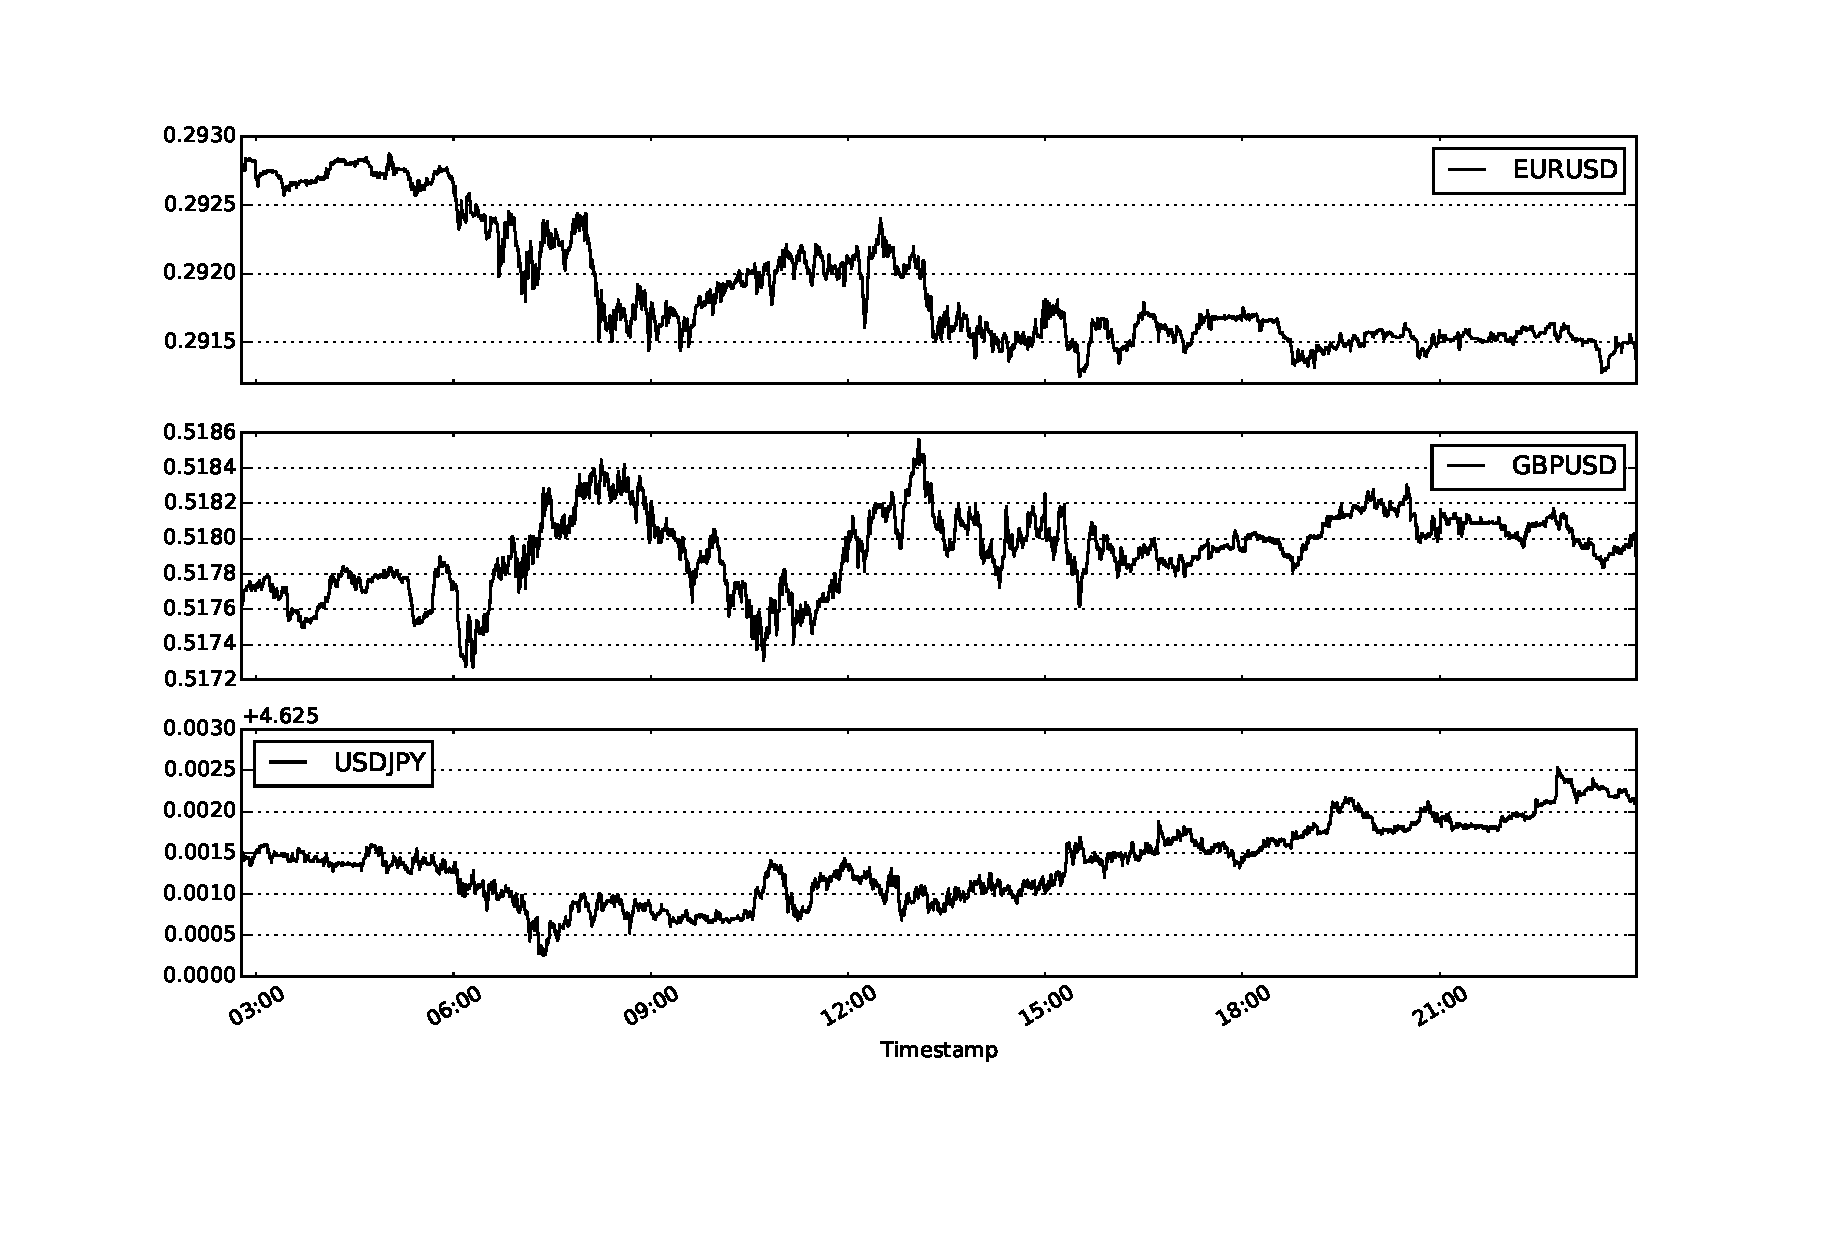
\includegraphics[width=\textwidth]{img/forexdata}
  \caption{10 seconds frequency forex data for EURUSD, GBPUSD and USDJPY}
  \label{fig:forexdata}
\end{figure}

\begin{figure}[!h]
  %\vspace{-0.8cm}
  \centering
  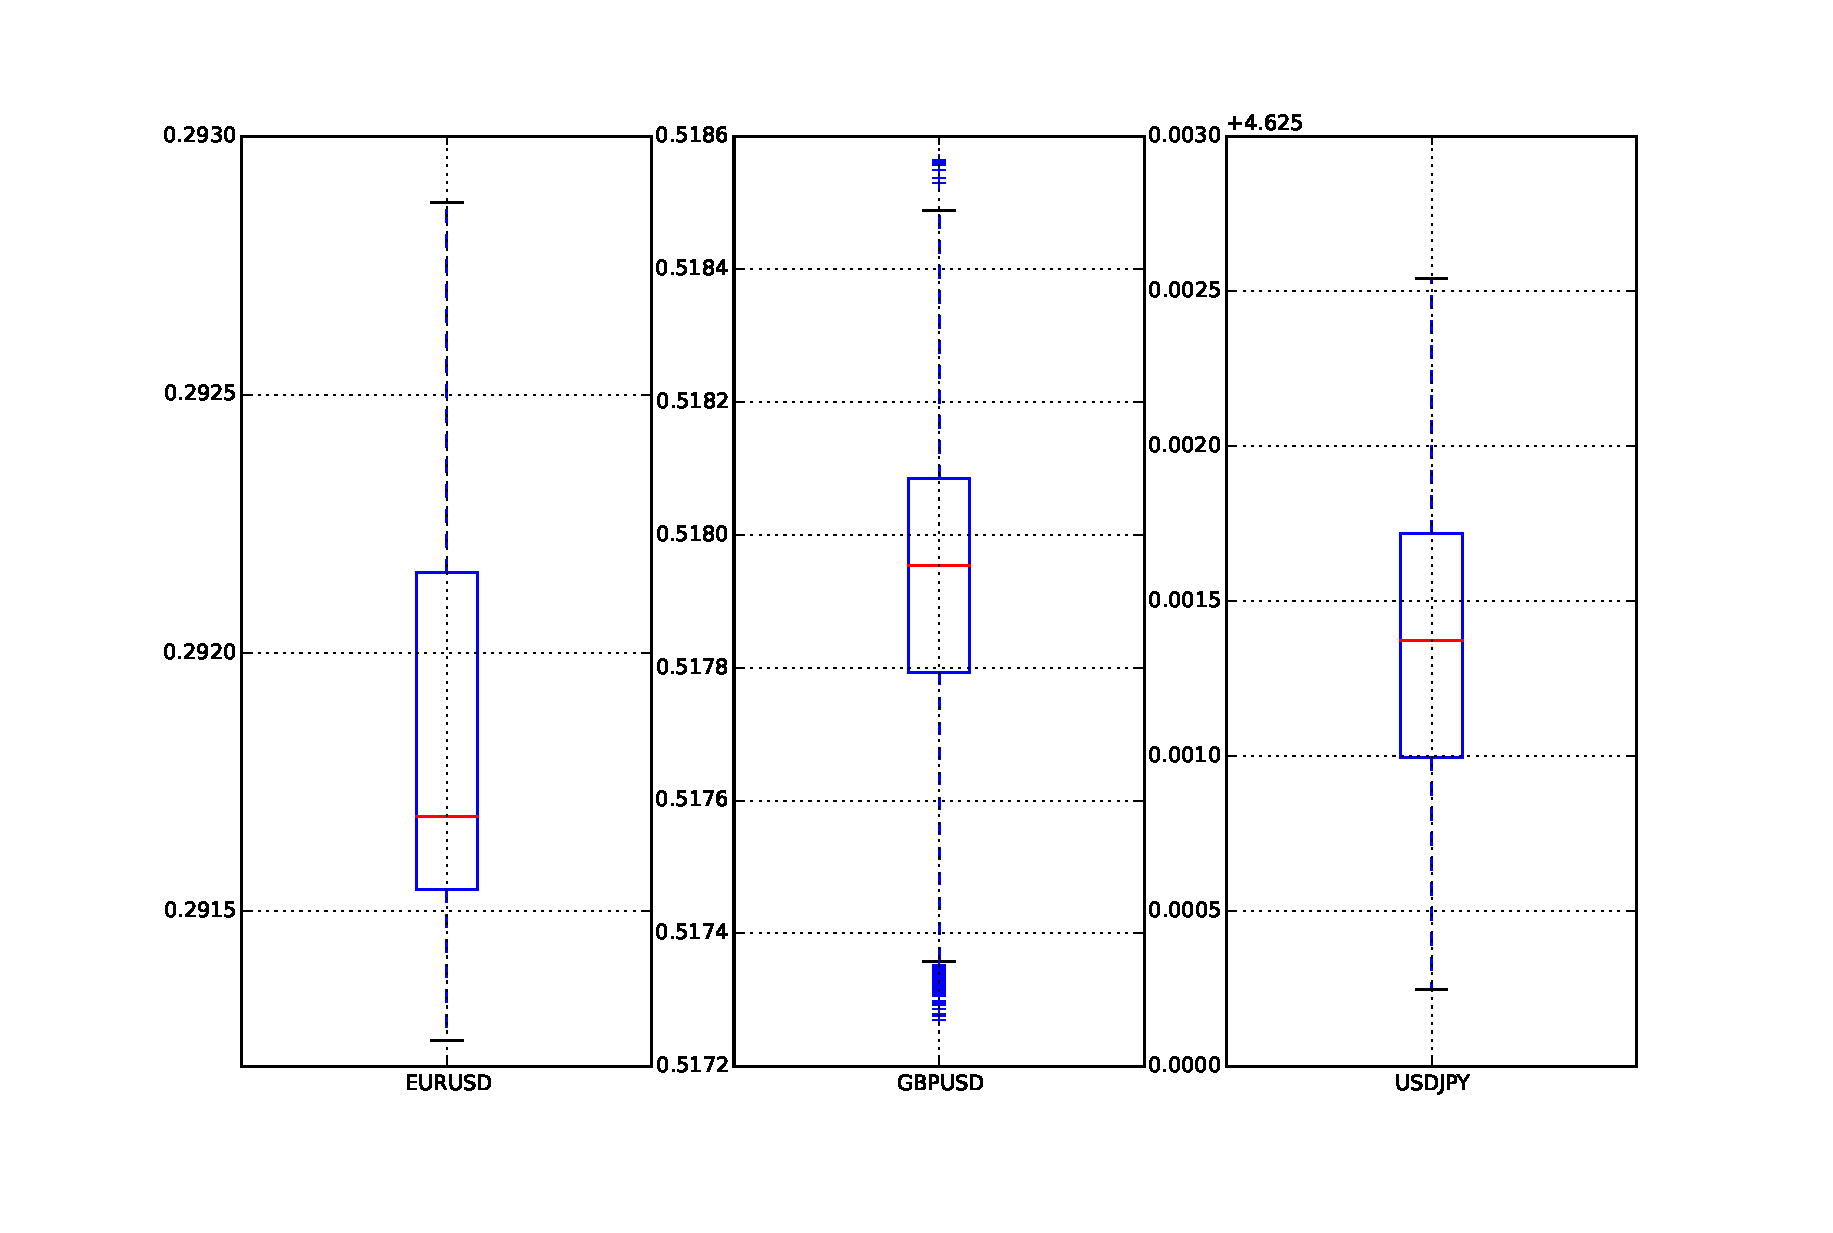
\includegraphics[width=0.8\textwidth]{img/distdata}
  \caption{Distribution of EURUSD, GBPUSD and USDJPY data}
  \label{fig:distdata}
\end{figure}


\begin{figure}[!h]
  %\vspace{-0.8cm}
  \centering
  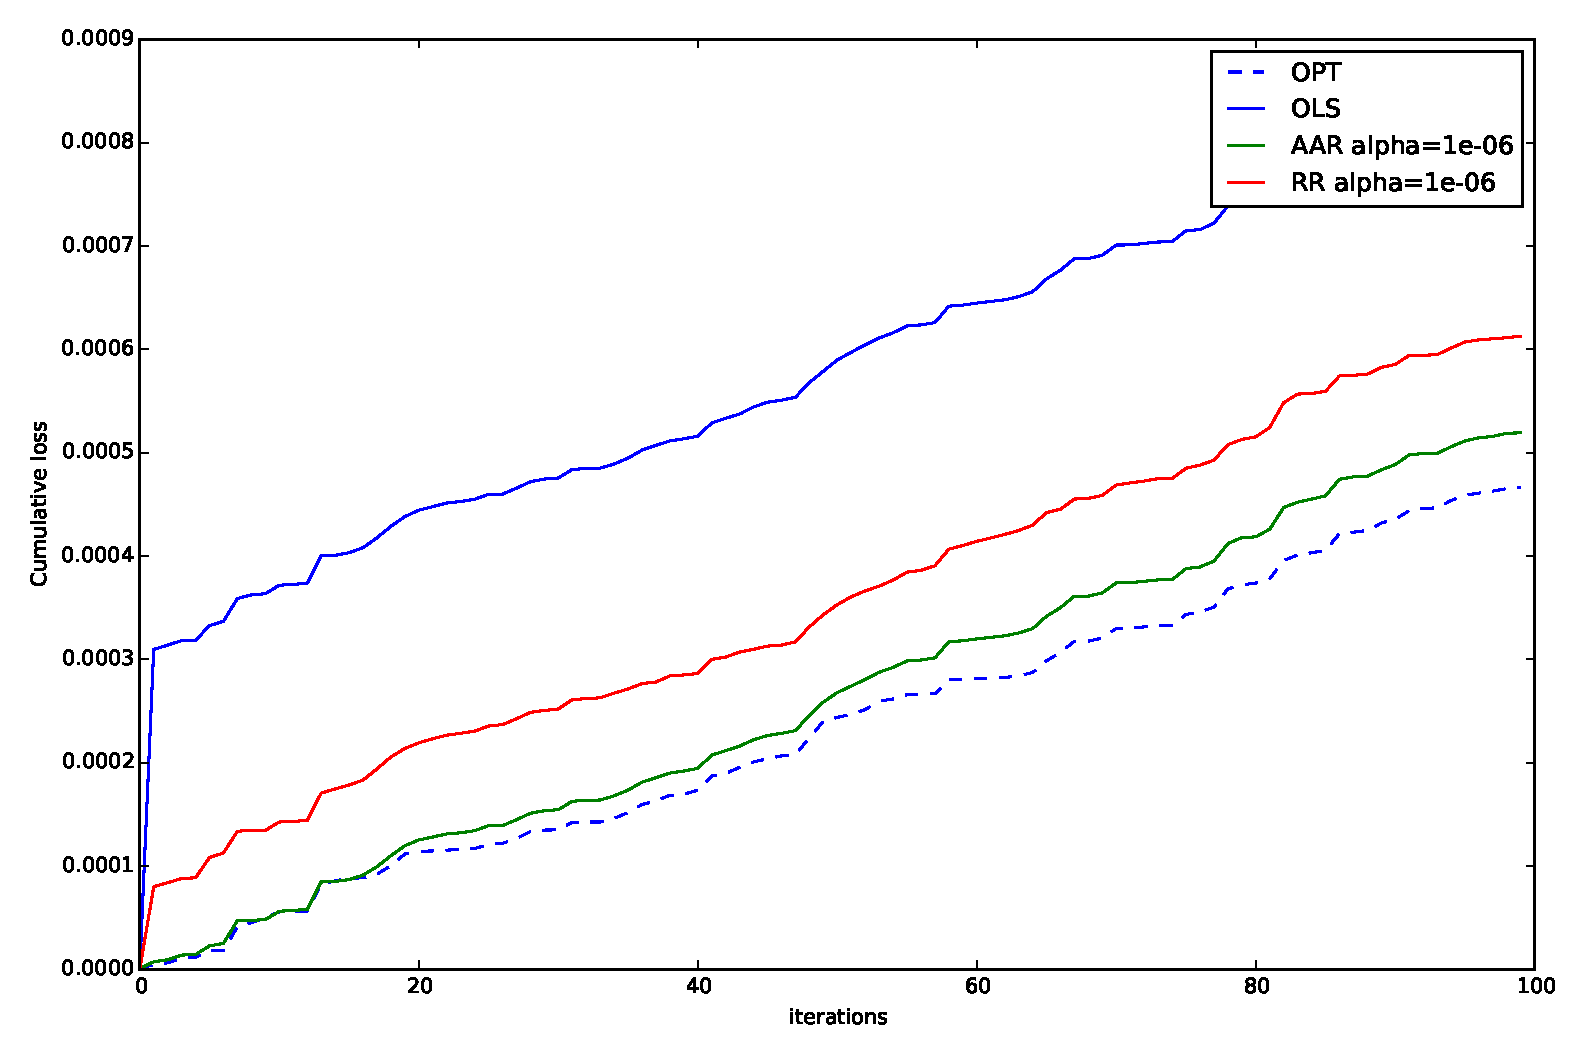
\includegraphics[width=0.9\textwidth]{img/onlinecomparison}
  \caption{Cumulative loss of AAR, RR and OLS solutions for VECM against its optimal algorithm}
  \label{fig:onlinecomparison}
\end{figure}


\begin{figure}[!h]
  %\vspace{-0.8cm}
  \centering
  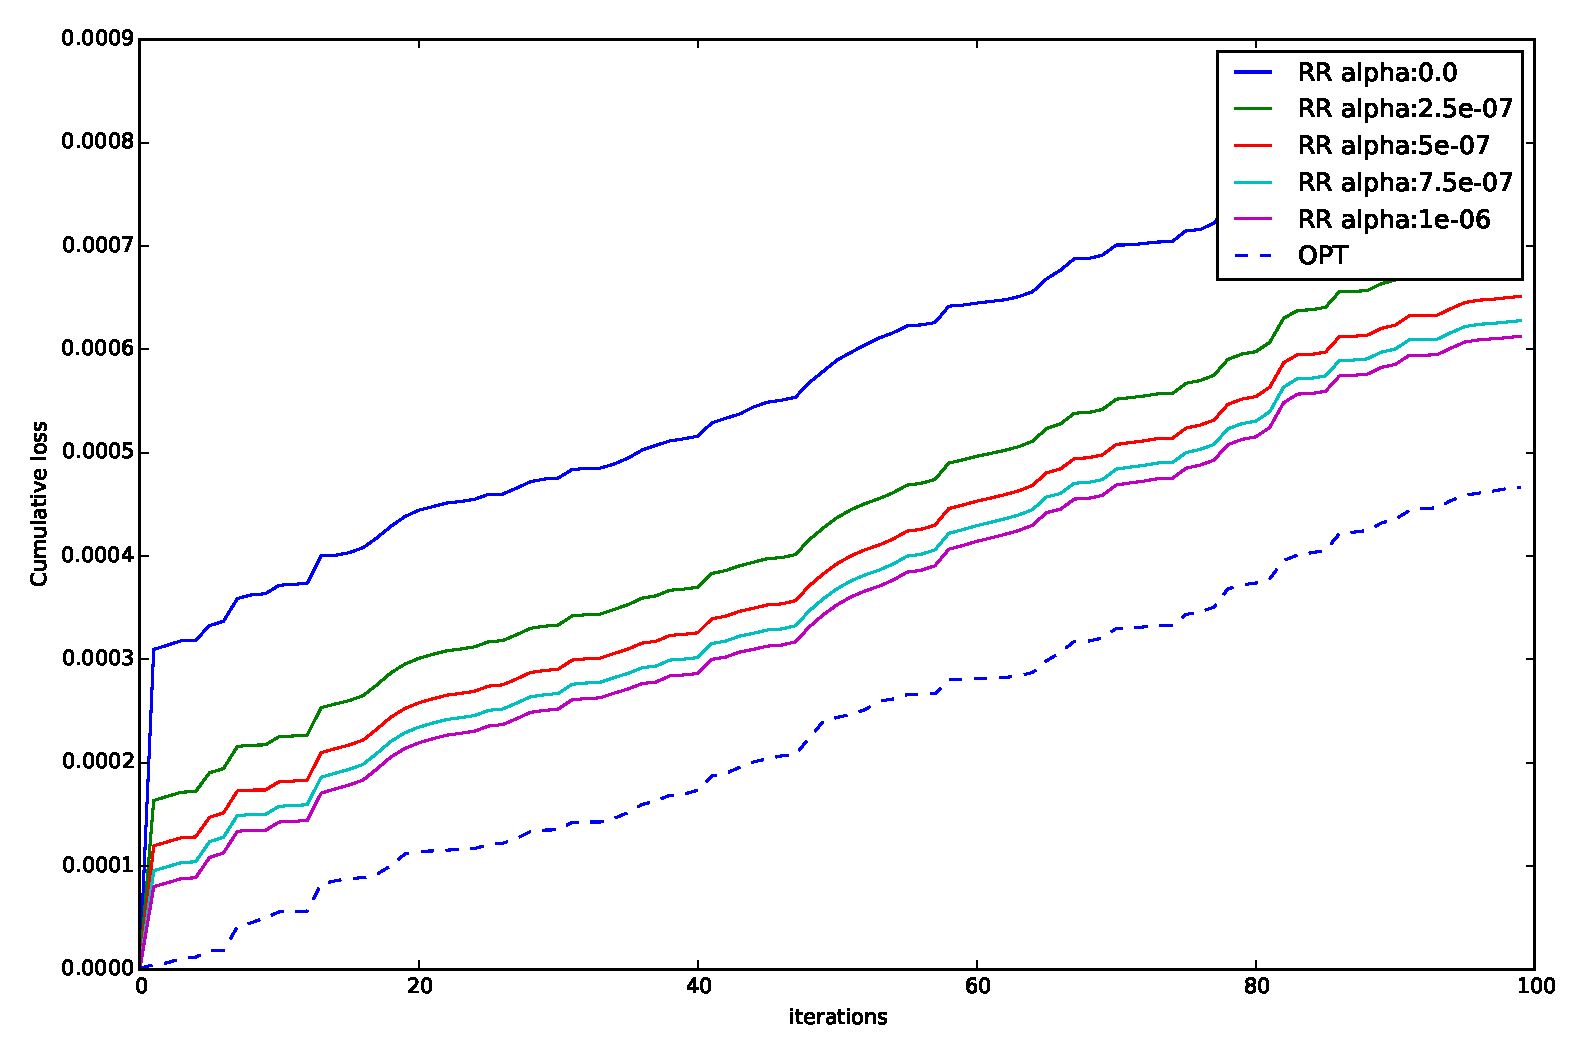
\includegraphics[width=0.9\textwidth]{img/RRcomparison}
  \caption{Cumulative loss RR VECM against its optimal algorithm using different $\lambda$ values}
  \label{fig:RRcomparison}
\end{figure}


\begin{figure}[!h]
  %\vspace{-0.8cm}
  \centering
  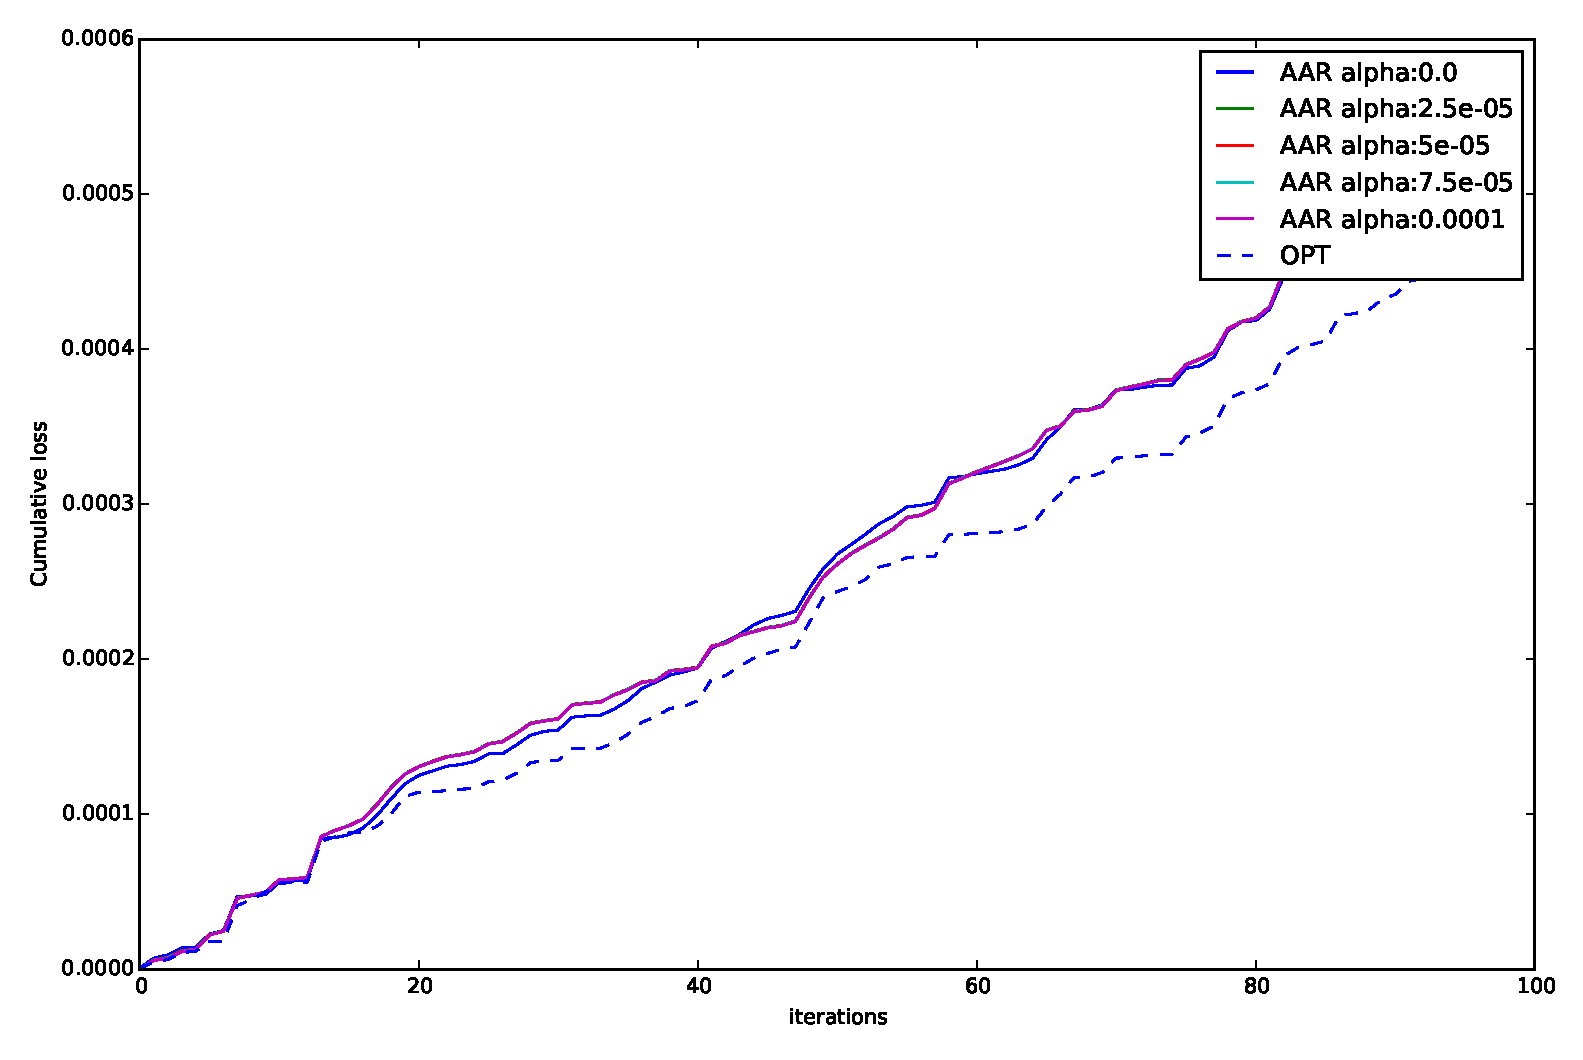
\includegraphics[width=0.9\textwidth]{img/AARcomparison}
  \caption{Cumulative loss AAR VECM against its optimal algorithm using different $\lambda$ values}
  \label{fig:AARcomparison}
\end{figure}



\chapter{Conclusions and Future Work}
\label{chapter:conclusions}
Main results and contributions are presented in this chapter along with some
suggested future work.

\vspace{0.5cm} 

\section{Conclusions of this thesis}

This thesis is a multidisciplinary work that involves knowledge of Finance
and Economics, Time Series, Machine Learning, Parallel Computing and Scientific
Computing. We specifically addressed the joint dynamic behaviour of financial time
series that are said to be cointegrated. A broadly used approach, called VECM (Vector
Error Correction Model), characterises this behaviour in terms of forces pulling
towards equilibrium called cointegration. However, the use of VECM has been
limited to low frequency time series processed in batch mode. In this thesis we
explored the use of VECM with high frequency data and we found that the main
limitation was computational. The focus of our work was developing a model to improve the performance forecasting of financial time series maintaining good execution times in order to use it with high frequency data. VECM parameter estimation uses two computationally
expensive routines: the Johansen method, to obtain cointegration vectors, and
the ordinary least squares method to solve the system. In this thesis, different
ways to explore cointegration in high frequency time series were proposed,
always considering the computational limitations of the VECM.

The study of cointegration in high frequency data was done using two different
approaches presented in Chapters \ref{chapter:proposal1} and
\ref{chapter:proposal2}, called AVECM and OVECM:
\begin{description}
\item[AVECM] AVECM is an adaptive version of VECM which includes a new method to choose VECM parameters based on
the maximisation of the percentage of cointegration. AVECM was implemented using
MPI to search on a grid of possible values. We evaluated our results in terms of performance and execution times:
\begin{description}
\item[Performance] Results showed that AVECM improves
performance measures by finding parameters of L and p maximising the percentage
of cointegration. AVECM performance was compared against ARIMA and the random walk model. We showed that the out-of-sample performance for AVECM is superior to ARIMA and the naive random walk model in terms of the MSE and $U$-statistic. This result is very important since it is still difficult to outperform ARIMA and the random walk model for standard econometric forecasting models  despite their simplicity. 
\item[Execution times] execution times were reduced more than 9 times
ensuring a response time before the processing of the next data point. Despite the fact that high frequency Forex data can be spurious, the model
performance can be less reliable (and more spurious) relative to the lower
frequencies (such as 1 minute or 5 minute intervals) adopted by some other
studies. However, the deficiency is offset by gain in accuracy from parallel
processing which is capable of searching or examining a much larger state space
given the same computational time.
\end{description}
\item[OVECM] We proposed an online version of VECM (OVECM). OVECM optimises how
model parameters are obtained using a sliding window of the most recent data.
OVECM, unlike AVECM, updates the parameters at each step, instead of obtaining
new ones. This proposal takes advantage of the long-run relationship
between the time series in order to obtain improved execution times. OVECM also
introduces matrix optimisation in order to obtain the new model in an iterative
way.  
\begin{description}
\item[Performance] 
OVECM was compared with the traditional VECM and ARIMA. Despite the fact that traditional VECM slightly outperformed our proposal, the OVECM execution time is lower. This result can be explained because OVECM avoids the calculation of cointegration vectors at each time step which improves execution times but can affect forecast performance.
\item[Execution times] OVECM was compared with the traditional VECM and ARIMA
with the same sliding window sizes. As a result, OVECM outperformed both in terms of
execution time. This reduction of execution time is mainly because OVECM avoids the cointegration vector calculation using the Johansen method. Aditionally, OVECM took much less than a minute at every
step making it possible to use with higher frequency data.  
\end{description}
\end{description}
Finally, cointegration information can now easily be used as an integration tool
to detect arbitrage opportunities or risk control in financial time series.

\section{Contributions of this thesis}

This research helped to integrate machine learning techniques and parallel computing with econometric models such as VECM so they can be used with high frequency data. We also observed that cointegration relationships are sensitive to the choice of the amount of data and VECM parameters and this can be used to improve forecasting performance. We proposed two variations of VECM, OVECM and AVECM which could be extended to other econometric models.

Regarding the initial objectives defined at the beginning of this thesis we can say:


\begin{itemize}
\item $\Large \mathcal{O}_1$: \emph{A review of the literature on time series
analysis models including machine learning techniques.}\\
The literature review was focused in finance, time series concepts and models and machine learning including theory and applications.
\item $\Large \mathcal{O}_2$: \emph{Development of a set of known features of the
studied time series and the application to improve forecasting.} \\
We included specific knowledge about forex rates, which were those used in our experiments, such as trade best trading times, stylised facts, percentage of cointegration, time series frequency, among others.
\item $\Large \mathcal{O}_3$: \emph{Development of parallel and efficient
algorithms to ensure quick response times .} \\
We showed that high performance computing will allow the use of computationally expensive methods to forecast high frequency data ensuring quick response times.
\item $\Large \mathcal{O}_4$: \emph{Deep mathematical analysis of the proposal
and financial concepts involved.} \\
The two proposals were presented with a strong mathematical foundation, we added definitions and proofs of all the concepts involved.
\item $\Large \mathcal{O}_5$: \emph{Design and implement representative set of
experiments in order to show when and why the proposal performs better.}
All the experiments were designed to give a general view of the method performance. We clearly showed the use and limitations of our proposals.
\end{itemize}


\section{Future Work}

For future study, it would be interesting to explore the relationship between
cointegration and performance for more assets, including not only forex rates
but also stocks. It would also be interesting to include more explaining
variables such as bid-ask spread and change in volume.

The online approach for other econometrics models it will be also worthy of 
study. Many of them could be adapted and used with higher frequency data. In
this thesis, the online version of OLS was studied, but the online version of
ridge regression could also be applied to obtain a solution with better
generalisation capabilities.

Financial time series are specially known for presenting high heteroscedasticity, common shocks in volatility could be wrongly interpreted as cointegration. To tackle this problem, a second step of the adaptive VECM algorithm could be implemented to the residuals. A good option could be a GARCH model, for example.  

Finally, it will be also interesting to improve the out-of-sample forecast
by considering more explicative variables, to increase window sizes or try different
conditions to obtain new cointegration vectors.



%%%%%%%%%%%%%%%%%%% APPENDIX %%%%%%%%%%%%%%%%%%%%%%%%%%%%

%\appendix
% Include appendix "chapters" here.
%\chapter{Proofs}
Some useful proofs for the understanding of this thesis.

\section{Pseudo-inverse computed using the compact SVD}\label{app:pscsvd}

\textbf{Proof}\quad

Since $\mathbf{A}$ is singular the problem shown in
equation~(\ref{eq:regressionproblem}) has not solution, the minimum norm given
by equation~(\ref{eq:MP}) is obtained by solving the equivalent problem:

\begin{equation*}
\label{eq:proyectorsol}
\mathbf{A \hat{X} = PB} 
\end{equation*}

\noindent where $\mathbf{P=U_1 U_1^\top}$ is the projection onto the
Col($\mathbf{A}$). 

Since $\mathbf{V} = [\underset{(n \times k)}{\mathbf{V_1}} |
\underset{(n \times k)}{\mathbf{V_2}}]$ and $\mathbf{V_1^\top V_2 =
0}$ we can express $\mathbf{\hat{X}} = \mathbf{V_1 x_1 + V_2 x_2}$
with $\mathbf{x_2=0}$ because $\mathbf{\hat{X}}$ lives in the
$\text{Row}(\mathbf{A})$ given by $\mathbf{V_1}$, so we have:

\begin{eqnarray*}
\mathbf{A \hat{X}} &=& \mathbf{PB} \\
\mathbf{U_1 \Sigma_1 V_1^\top \hat{X}} &=& \mathbf{U_1 U_1^\top B} \\
\mathbf{ V_1^\top \hat{X}} &=&  \mathbf{\Sigma_1^{-1} U_1^\top B} \\ 
\mathbf{ V_1^\top V_1 x_1} &=& \mathbf{\Sigma_1^{-1}
U_1^\top B} \\
\mathbf{x_1}&=& \mathbf{\Sigma_1^{-1} U_1^\top B}
\end{eqnarray*}

\noindent from this result we can obtain $\mathbf{\hat{X}}$ and
therefore the pseudo-inverse expression:

\begin{eqnarray*}
\mathbf{\hat{X}} &=& \mathbf{V_1 x_1} \\
                &=& \mathbf{V_1 \Sigma_1^{-1} U_1^\top B} \\
\mathbf{A^+} &=& \mathbf{V_1 \Sigma_1^{-1} U_1^\top} \, .
\end{eqnarray*}

$\blacksquare$

\section{The pseudo-inverse computed using the compact
singular value decomposition (SVD)} \label{app:pseudoproof}
\begin{equation}
\mathbf{A}^+ = \mathbf{V_1\Sigma_1^{-1}U_1^\top}
\end{equation}

\textbf{Proof}\quad

In the case matrix $\mathbf{A}$ is non singular, its solution is
straight forward:

\begin{equation}
\label{OLSsolution2}
    \mathbf{\mathbf{X}}=\mathbf{A}^{-1}\mathbf{Y}
\end{equation}


Since the problem shown in equation~(\ref{eq:regproblem}) has not
solution, the minimum norm given by equation~(\ref{OLSsolution2}) is
obtained by solving the equivalent problem:

\begin{equation*}
\label{eq:proyectorsol}
\mathbf{A \hat{\mathbf{X}} = PY} 
\end{equation*}


\noindent where $\mathbf{P=U_1 U_1^\top}$ is the projection onto the
Col($\mathbf{A}$). 

Since $\mathbf{V} = [\underset{(n \times k)}{\mathbf{V_1}} |
\underset{(n \times k)}{\mathbf{V_2}}]$ and $\mathbf{V_1^\top V_2 =
0}$ we can express $\mathbf{\hat{\mathbf{X}}} = \mathbf{V_1 \mathbf{X}_1 + V_2 \mathbf{X}_2}$
with $\mathbf{\mathbf{X}_2=0}$ because $\mathbf{\hat{\mathbf{X}}}$ lives in the
$\text{Row}(\mathbf{A})$ given by $\mathbf{V_1}$, so we have:

\begin{eqnarray*}
\mathbf{A \hat{\mathbf{X}}} &=& \mathbf{PY} \\
\mathbf{U_1 \Sigma_1 V_1^\top \hat{\mathbf{X}}} &=& \mathbf{U_1 U_1^\top Y} \\
\mathbf{ V_1^\top \hat{\mathbf{X}}} &=&  \mathbf{\Sigma_1^{-1} U_1^\top Y} \\ 
\mathbf{ V_1^\top V_1 \mathbf{X}_1} &=& \mathbf{\Sigma_1^{-1}
U_1^\top Y} \\
\mathbf{\mathbf{X}_1}&=& \mathbf{\Sigma_1^{-1} U_1^\top Y}
\end{eqnarray*}

\noindent from this result we can obtain $\mathbf{\hat{\mathbf{X}}}$ and
therefore the pseudo-inverse expression:

\begin{eqnarray*}
\mathbf{\hat{\mathbf{X}}} &=& \mathbf{V_1 \mathbf{X}_1} \\
                &=& \mathbf{V_1 \Sigma_1^{-1} U_1^\top Y} \\
\mathbf{A^+} &=& \mathbf{V_1 \Sigma_1^{-1} U_1^\top} \, .
\end{eqnarray*}

$\blacksquare$

\section{Ridge regression optimal solution}\label{app:rroptsection}

\begin{equation*}
\mathbf{\mathbf{X}}_*=(\mathbf{A}^\top \mathbf{A}+\lambda \mathbb{I})^{-1}\mathbf{A}^\top y \, ,
\end{equation*}


\textbf{Proof}\quad

\begin{eqnarray*}
J(\mathbf{\mathbf{X}}) &=&  \| \mathbf{A}\mathbf{\mathbf{X}} - \mathbf{Y} \|_2^2  + \lambda
 \| \mathbf{\mathbf{X}}\| ^2 \\
 &=&  \sum_{t=1}^N (\mathbf{\mathbf{X}}^\top {\bf a}_t-y_t)^2 + \lambda \sum_{i=1}^p \mathbf{X}_i^2 \\
 &=& (\mathbf{X}^\top a_1-y_1)^2 + \dots + (\mathbf{X}^\top a_N-y_N)^2 + \lambda (\mathbf{X}_1^2+\dots+\mathbf{X}_p^2)
\end{eqnarray*}
\noindent taking derivatives
 \begin{eqnarray*}
 \frac{\partial J(\mathbf{\mathbf{X}})}{\partial \mathbf{X}_1}&=& 
 2(\mathbf{X}^\top \mathbf{a}_1-y_1)\mathbf{a}_{11} + \dots + 2(\mathbf{X}^\top \mathbf{a}_N-y_N)\mathbf{a}_{N1} + 2\lambda \mathbf{X}_1 \\
 &=& 2\mathbf{a}_1^\top(\mathbf{A}\mathbf{X}-\mathbf{Y}) + 2\lambda\mathbf{X}_1\\
& \vdots &\\
  \frac{\partial J(\mathbf{\mathbf{X}})}{\partial \mathbf{X}_p}&=& 
 2\mathbf{a}_p^\top(\mathbf{A}\mathbf{X}-\mathbf{Y}) + 2\lambda\mathbf{X}_p 
\end{eqnarray*}

Then we have that:
\begin{eqnarray*}
\frac{\partial J(\mathbf{\mathbf{X}})}{\partial \mathbf{X}}&=& 
 2\mathbf{A}^\top(\mathbf{A}\mathbf{X}-\mathbf{Y}) + 2\lambda\mathbf{X}
\end{eqnarray*}
Since $\frac{\partial J(\mathbf{\mathbf{X}})}{\partial \mathbf{X}}=0$ we have:
\begin{eqnarray*}
2\mathbf{A}^\top(\mathbf{A}\mathbf{X}-\mathbf{Y}) + 2\lambda\mathbf{X}&=&0 \\
\mathbf{A}^\top\mathbf{A}\mathbf{X} - \mathbf{A}^\top\mathbf{Y} + \lambda\mathbf{X} &=& 0\\
(\mathbf{A}^\top\mathbf{A}+\lambda\mathbb{I})\mathbf{X} &=&  \mathbf{A}^\top\mathbf{Y} \\
\mathbf{X} &=& (\mathbf{A}^\top\mathbf{A}+\lambda\mathbb{I})^{-1}  \mathbf{A}^\top\mathbf{Y}
\end{eqnarray*}

$\blacksquare$

\section{Bias and Variance}\label{app:biasandvariance}

The OLS bias can be obtained as:

\begin{eqnarray*}
Bias(\hat{f}(\hat{\mathbf{X}})) &=& E[\hat{\mathbf{X}}] - \mathbf{X} \\
&=& E[ (\mathbf{A}^\top \mathbf{A})^{-1}\mathbf{A}^\top \mathbf{Y}] - \mathbf{X} \\
&=& E[ (\mathbf{A}^\top \mathbf{A})^{-1}\mathbf{A}^\top (\mathbf{AX})] - \mathbf{X}  \\
&=& \mathbf{X}  - \mathbf{X}  \\
&=&  0
\end{eqnarray*}

The Ridge Regression bias can be obtained as:

\begin{eqnarray*}
\mathbf{X}(\lambda) &=&( \mathbf{A}^\top \mathbf{A} + \lambda \mathbb{I})^{-1}\mathbf{A}^\top \mathbf{Y} \\
&=& (\mathbb{I} + \lambda (\mathbf{A}^\top \mathbf{A})^{-1})^{-1} (\mathbf{A}^\top \mathbf{A})^{-1}\mathbf{A}^\top \mathbf{Y} \\
&=&  (\mathbb{I} + \lambda (\mathbf{A}^\top \mathbf{A})^{-1})^{-1}  \hat{\mathbf{X}} \\
&=& \mathbf{W} \hat{\mathbf{X}} 
\end{eqnarray*}

\noindent where $\mathbf{W}  = (\mathbb{I} + \lambda (\mathbf{A}^\top
\mathbf{A})^{-1})^{-1}  $ it is defined for simplicity. Ridge
regression bias is then obtained as:

\begin{eqnarray*}
Bias(\mathbf{X}(\lambda)) &=& E[\mathbf{X}(\lambda)] - \mathbf{X} \\
&=& E[\mathbf{W}\hat{\mathbf{X}}] - \mathbf{X} \\
&=&  \mathbf{W} \mathbf{X} - \mathbf{X} \neq 0 
\end{eqnarray*}


The variance of OLS is:

\begin{equation*}
Var(\hat{\mathbf{X}}) = \sigma^2 (\mathbf{A}^\top \mathbf{A} )^{-1}
\end{equation*}

\noindent and the variance of ridge regression is:

\begin{eqnarray*}
Var(\mathbf{X}(\lambda)) &=& Var(\mathbf{W}\hat{\mathbf{X}}) \\
&=& E[(\mathbf{W}\hat{\mathbf{X}}-E[\mathbf{W}\hat{\mathbf{X}}])(\mathbf{W}\hat{\mathbf{X}}-E[\mathbf{W}\hat{\mathbf{X}}])^\top] \\
&=& \mathbf{W}E[(\hat{\mathbf{X}}-E[\hat{\mathbf{X}}])(\hat{\mathbf{X}}-E[\hat{\mathbf{X}}])^\top] \mathbf{W}^\top \\
&=& \mathbf{W}Var(\hat{\mathbf{X}})\mathbf{W}^\top \\
&=& \sigma^2 \mathbf{W}(\mathbf{A}^\top \mathbf{A} )^{-1}\mathbf{W}^\top
\end{eqnarray*}

\section{Ridge regression shows an
increasing squared bias and a decreasing variance} \label{app:rrbiasvar}

\textbf{Proof}\quad

Since $Bias(\mathbf{X}(\lambda)) \neq 0$ this imply that

\begin{equation*}
Bias(\mathbf{X}(\lambda)) ^2 > 0 
\end{equation*}

\noindent we know that $\mathbf{A}^\top
\mathbf{A}$ has an eigenvalue decomposition $\mathbf{A}^\top
\mathbf{A} = \mathbf{V} \Sigma \mathbf{V}^{-1}$.


\begin{eqnarray*}
Var(\mathbf{X}(\lambda)) &=& \sigma^2 \mathbf{W}(\mathbf{A}^\top \mathbf{A} )^{-1}\mathbf{W}^\top\\
Var(\mathbf{X}(\lambda)) &=& \sigma^2 (\mathbb{I} + \lambda (\mathbf{A}^\top
\mathbf{A})^{-1})^{-1} (\mathbf{A}^\top \mathbf{A} )^{-1}((\mathbb{I} + \lambda (\mathbf{A}^\top
\mathbf{A})^{-1})^{-1} )^\top \\
&=& \sigma^2 (\mathbb{I} + \lambda (\mathbf{V} \Sigma \mathbf{V}^{-1})^{-1} (\mathbf{V} \Sigma \mathbf{V}^{-1})^{-1}((\mathbb{I} + \lambda (\mathbf{V} \Sigma \mathbf{V}^{-1})^{-1})^{-1} )^\top \\
&=& \sigma^2 \mathbf{V} (\mathbb{I} + \lambda \Sigma^{-1})^{-1} \Sigma^{-1} (\mathbb{I} + \lambda \Sigma^{-1})^{-1}  \mathbf{V}^{-1}\\
&=& \sigma^2 \mathbf{V} \mathbf{D}^{-1} \mathbf{V}^{-1}
\end{eqnarray*}

\noindent where $\mathbf{D}^{-1}  = (\mathbb{I} + \lambda \Sigma^{-1})^{-1} \Sigma^{-1} (\mathbb{I} + \lambda \Sigma^{-1})^{-1}$ is a diagonal matrix with coefficients:

\begin{equation*}
d_i = \frac{\sigma_i^{-1}}{(1+\lambda\sigma_i^{-1})^2}
\end{equation*}

$\blacksquare$

\section{Efficient computation}\label{app:effcomp}
In regression problems we always require getting a matrix inverse which is
computationally expensive. However, in stream data problems there is a way to
obtain a matrix inverse approximation using the Sherman-Morrison-Woodbury. This
formula allows to get the inverse of a matrix $\mathbf{A+uv^\top}$ if we previously calculated the
inverse of $\mathbf{A}$ as follows:

\begin{equation}
\label{eq:SMW}
(\mathbf{A+uv^\top})^{-1}=\mathbf{A}^{-1}-
\frac{\mathbf{A^{-1}uv^\top A^{-1}}}{\mathbf{1+v^\top A^{-1}u}}
\end{equation}


Alternatively, Coleman and
Sun~\cite{coleman+sun2010} presented an iterative algorithm which
uses $\mathbf{X}(\lambda)$ to approximate $\mathbf{X}(0)$.


Using the compact SVD (shown in equation~(\ref{eq:compactsvd}))
$\mathbf{X}(\lambda)$ is expressed as follows:


\begin{eqnarray}
\label{eq:optsolRRsvd}
\mathbf{X}(\lambda) & = & (\mathbf{A}^\top \mathbf{A}+ \lambda
\mathbb{I})^{-1}\mathbf{A}^\top \mathbf{Y} \nonumber \\
& = &\mathbf{V}_1(\Sigma_1^2+\lambda \mathbb{I})^{-1}\mathbf{\Sigma_1
U_1^\top Y}
\end{eqnarray}

\noindent where is easy to see that $\mathbf{X}(\lambda) \rightarrow
\mathbf{\hat{X}}=\mathbf{V}_1 \mathbf{\Sigma}_1^{-1}\mathbf{U}_1^\top
\mathbf{Y}$ as $\lambda \rightarrow 0$. 

The method consists in obtaining $\mathbf{X}(\lambda)$ and then refine
by adding more terms of its Taylor expansion to approximate
$\mathbf{X}(0) = \mathbf{\hat{X}}$. The Taylor expansion about $\lambda_0$ is:

\begin{equation}
\label{eq:taylor}
    \mathbf{X}(\lambda)=\mathbf{X}(\lambda_0) + \sum_{k=1}^\infty
    \mathbf{s}_k(\lambda-\lambda_0)^{k}
\end{equation}


\noindent where $\mathbf{s}_k=\frac{1}{k!}\mathbf{X}(\lambda)^{(k)}$
and $\mathbf{X}(\lambda)^{(k)}$ is obtained by taking differences 
$\frac{\partial}{\partial \lambda}$ of:  

\begin{eqnarray*}
(\mathbf{A}^\top \mathbf{A}+ \lambda\mathbb{I}) \mathbf{X}(\lambda) & = & \mathbf{A}^\top \mathbf{Y}\\
(\mathbf{A}^\top \mathbf{A}+ \lambda\mathbb{I}) \mathbf{X}(\lambda)^{(1)} + \mathbf{X}(\lambda)& = & 0 \\
\mathbf{X}(\lambda)^{(1)}  &=& -(\mathbf{A}^\top \mathbf{A}+ \lambda\mathbb{I}) ^{-1} \mathbf{X}(\lambda) \\
\mathbf{X}(\lambda)^{(2)}  &=& -2(\mathbf{A}^\top \mathbf{A}+ \lambda\mathbb{I}) ^{-1} \mathbf{X}(\lambda)^{(1)} \\
& \vdots & \\
\mathbf{X}(\lambda)^{(k)}  &=& -k(\mathbf{A}^\top \mathbf{A}+ \lambda\mathbb{I}) ^{-1} \mathbf{X}(\lambda)^{(k-1)} 
\end{eqnarray*}



\noindent for $\lambda=0$ we have:

\begin{equation}
\label{eq:taylor}
    \mathbf{X}(0)=\mathbf{X}(\lambda_0) + \sum_{k=1}^\infty
     (-1)^k \mathbf{s}_k \lambda_0^k
\end{equation}


\noindent therefore in order to ensure convergence, we can see that $\lambda_0$ cannot be large. 

The algorithm for computing $\mathbf{X}(0)$ is the following:

\begin{algorithm}[H]
\begin{algorithmic}[1]
\REQUIRE $\,$ \\
$\mathbf{A}$: design matrix \\
$\mathbf{Y}$: response matrix \\
$\lambda$: rank deficient parameter \\
\ENSURE  $\,$ \\
$\mathbf{X}$: parameters \\
\STATE $\mathbf{M}=\mathbf{A^\top A}$ \\
\STATE Initialize $\mathbf{Q R}=\mathbf{M}$ \\
\STATE $\mathbf{X} = \mathbf{R^{-1}Q^\top Y}$ \\
\STATE $\mathbf{s} = \mathbf{X}$ \\
\FOR { $i = 1,2,3,\dots$ }
	\STATE $\mathbf{s} =
        -(\mathbf{M}+\lambda\mathbb{I})^{-1}\mathbf{s}$\\
	\STATE $\mathbf{X}=\mathbf{X} + (-1)^i {\color{red}\mathbf{s}
        \lambda^i}$
\ENDFOR
\end{algorithmic}
\caption{Algorithm for handling rank deficient matrices}
\label{alg:coleman}
\end{algorithm}

The algorithm~\ref{alg:coleman} solves equation~(\ref{eq:taylor}). However, this
version is unstable since typically $\|\mathbf{s}\|$ is very large and
$\lambda^i$ is very small ($\lambda$ is small).

The following algorithm shows a more stable version of
algorithm~\ref{alg:coleman}.


\begin{algorithm}[H]
\begin{algorithmic}[1]
\REQUIRE $\,$ \\
$\mathbf{A}$: design matrix \\
$\mathbf{Y}$: response matrix \\
$\lambda$: rank deficient parameter \\
\ENSURE  $\,$ \\
$\mathbf{X}$: parameters \\
\STATE $\mathbf{M}=\mathbf{A^\top A}$ \\
\STATE Initialize $\mathbf{Q R}=\mathbf{M}$ \\
\STATE $\mathbf{X} = \mathbf{R^{-1}Q^\top Y}$ \\
\STATE $\mathbf{t} = \mathbf{X}$ \\
\FOR { $i = 1,2,3,\dots$ }
        \STATE $\mathbf{t} =\lambda \mathbf{t}$  
        \STATE $\mathbf{t} =  -(\mathbf{M}+\lambda\mathbb{I})^{-1}\mathbf{t}$
	\STATE $\mathbf{X}=\mathbf{X} + \mathbf{t}$
\ENDFOR
\end{algorithmic}
\caption{Algorithm for handling rank deficient matrices improved}
\label{alg:colemanimproved}
\end{algorithm}

Both algorithms are equivalent, but algorithm~\ref{alg:colemanimproved} is more
stable and converges in typically less than 10 steps.
It is important to notice that the QR factorisation is computed only once and it
is computationally less expensive than the SVD.



%%%%%%%%%%%%%%%%%%% BACK MATTER %%%%%%%%%%%%%%%%%%%%%%%%%%%%

\backmatter
% Bibliography styles amsplain or harvard are also acceptable.
\bibliographystyle{amscls/amsalpha}
\bibliography{reference}
%    See note above about multiple indexes.
\printindex

\end{document}

%-----------------------------------------------------------------------
% End of amsbook.template
%-----------------------------------------------------------------------

